\section{Preventivo}
In questa sezione del documento viene riportata la distribuzione delle risorse del gruppo nelle varie fasi di lavoro.\\
Inoltre sono illustrate la pianificazione e distribuzione oraria dei ruoli per ogni membro del gruppo, i quali devono:
\begin{itemize}
	\item Ricoprire tutti i ruoli durante tutta la durata del progetto;
	\item Avere circa le stesse ore produttive alla fine di ogni fase del progetto.
\end{itemize}
Inoltre il verificatore di un determinato task\textsubscript{G} non potrà essere colui che lo ha svolto.\\
Il riferimento alle sigle identificative dei ruoli si può trovare al paragrafo 3.1.5.5 del documento \textbf{Norme di progetto v0.0.7}.
\newpage
\subsection{Analisi}
%
% ----------------------------------------------------------------------------------------------------------------
\subsubsection{Periodo 1}
% ----------------------------------------------------------------------------------------------------------------
%
\subsubsubsection{Preventivo orario}
La seguente tabella rappresenta la distribuzione oraria per ogni componente per il primo periodo della fase di Analisi:

	\setlength\extrarowheight{5pt}
	\rowcolors{2}{gray!10}{gray!40}
	\begin{tabularx}{\textwidth}{|ccccccc|c|}
		\hline
		\rowcolor{white}
		\textbf{Nome} & \textbf{Re} & \textbf{Am} & \textbf{An} & \textbf{Ve} & \textbf{Pr}& \textbf{Pt} & \textbf{Ore totali} \\
		\hline
		Nicola Sinicato &3&3&4&0&0&0&10 \\
		Gabriele Da Re &0&6&4&0&0&0&10 \\
		Luca Brugnera &0&6&4&0&0&0&10 \\
		Matteo Stocco &1&5&4&0&0&0&10 \\
		Ana Lazic &1&3&6&0&0&0&10 \\
		Zhen Wei Zheng &1&3&6&0&0&0&10 \\
		\hline
		Ore totali ruolo &6&26&28&0&0&0&60 \\
		\hline
		\rowcolor{white}
		\caption{ Distribuzione oraria durante il primo periodo di analisi per ruolo e persona}
	\end{tabularx}
	\vspace{10pt}
	

\begin{figure}[H]
    \centering
    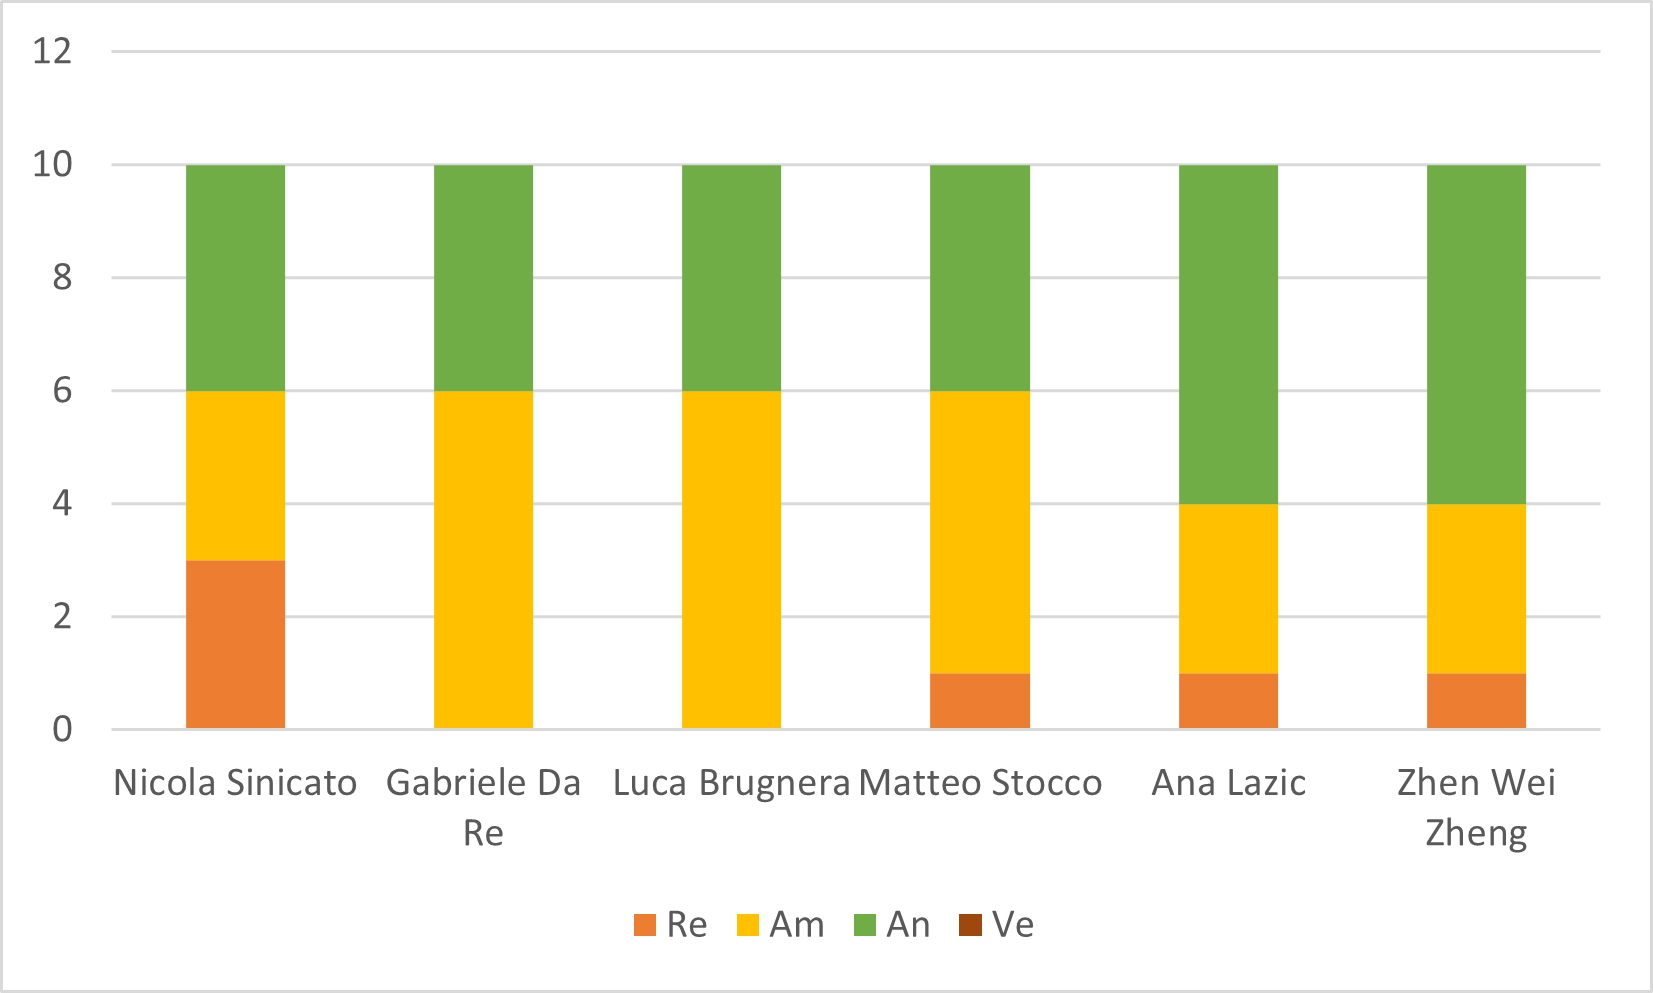
\includegraphics[scale=0.6]{img/grafi preventivo/istogrammi/analisi/periodo1.png}
    \caption{Istogramma della ripartizione delle ore del primo periodo della fase di analisi}
\end{figure}
\begin{figure}[H]
    \centering
    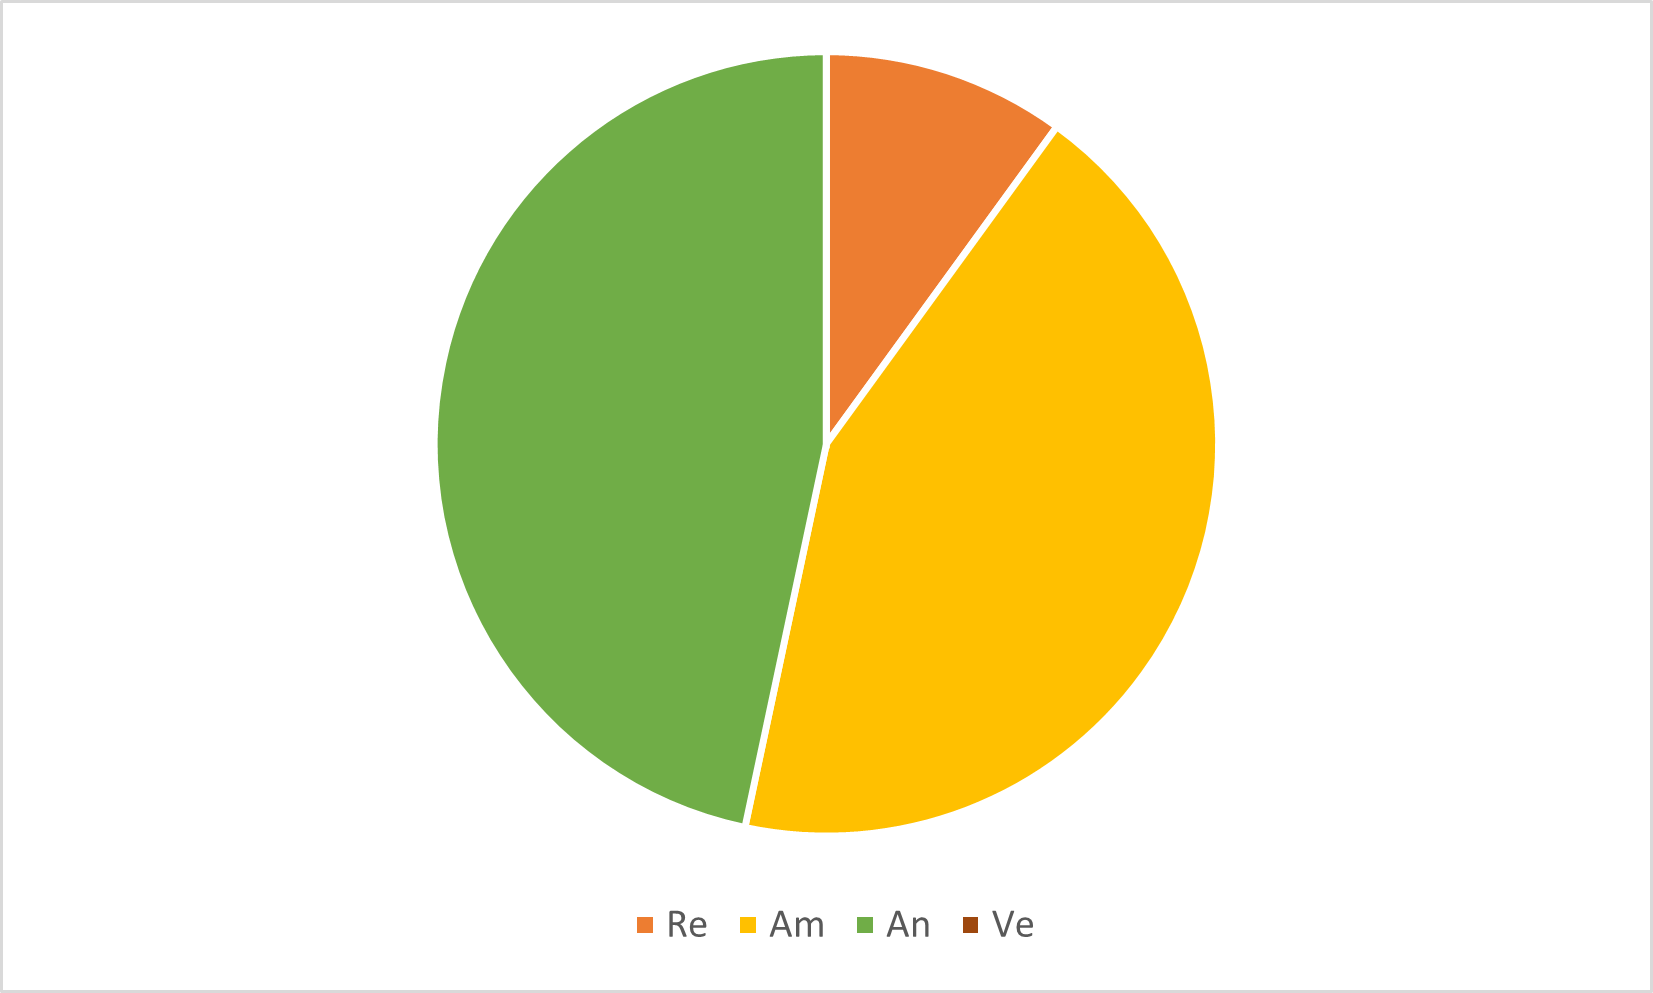
\includegraphics[scale=0.6]{img/grafi preventivo/torta/analisi/periodo1.png}
    \caption{Grafico a torta della ripartizione delle ore per ruolo nel primo periodo della fase di analisi}
\end{figure}

\subsubsubsection{Preventivo dei costi}
La seguente tabella rappresenta le ore dedicate ad ogni ruolo e il corrispettivo costo in euro per il primo periodo della fase di analisi:

	\setlength\extrarowheight{5pt}
	\rowcolors{2}{gray!10}{gray!40}
	\begin{tabularx}{\textwidth}{|ccc|c|}
		\hline
		\rowcolor{white}
		\textbf{Ruolo} & \textbf{Costo orario (€)} & \textbf{Ore totali} & \textbf{Costo totale (€)} \\
		\hline
		Responsabile &30&6&180 \\
		Amministratore &20&26&520 \\
		Analista &25&28&700 \\
		Verificatore &15&0&0 \\
		Programmatore &15&0&0 \\
		Progettista &25&0&0 \\
		\hline
		Totale &-&-&1400 \\
		\hline
		\rowcolor{white}
		\caption{Prospetto del costo orario durante il primo periodo di analisi per ruolo}
	\end{tabularx}
    \vspace{10pt}
	
% ----------------------------------------------------------------------------------------------------------------
\newpage
\subsubsection{Periodo 2}
% ----------------------------------------------------------------------------------------------------------------
%
\subsubsubsection{Preventivo orario}
La seguente tabella rappresenta la distribuzione oraria per ogni componente per il secondo periodo della fase di analisi:

	\setlength\extrarowheight{5pt}
	\rowcolors{2}{gray!10}{gray!40}
	\begin{tabularx}{\textwidth}{|ccccccc|c|}
		\hline
		\rowcolor{white}
		\textbf{Nome} & \textbf{Re} & \textbf{Am} & \textbf{An} & \textbf{Ve} & \textbf{Pr}& \textbf{Pt} & \textbf{Ore totali} \\
		\hline
		Nicola Sinicato &2&1&8&4&0&0&15 \\
		Gabriele Da Re &1&4&7&3&0&0&15 \\
		Luca Brugnera &1&5&6&3&0&0&15 \\
		Matteo Stocco &2&2&7&4&0&0&15 \\
		Ana Lazic &0&2&7&6&0&0&15 \\
		Zhen Wei Zheng &0&2&6&7&0&0&15 \\
		\hline
		Ore totali ruolo &6&16&41&27&0&0&90 \\
		\hline
		\rowcolor{white}
		\caption{Distribuzione oraria durante il secondo periodo di analisi per ruolo e persona}
	\end{tabularx}
	\vspace{10pt}
	
\begin{figure}[H]
    \centering
    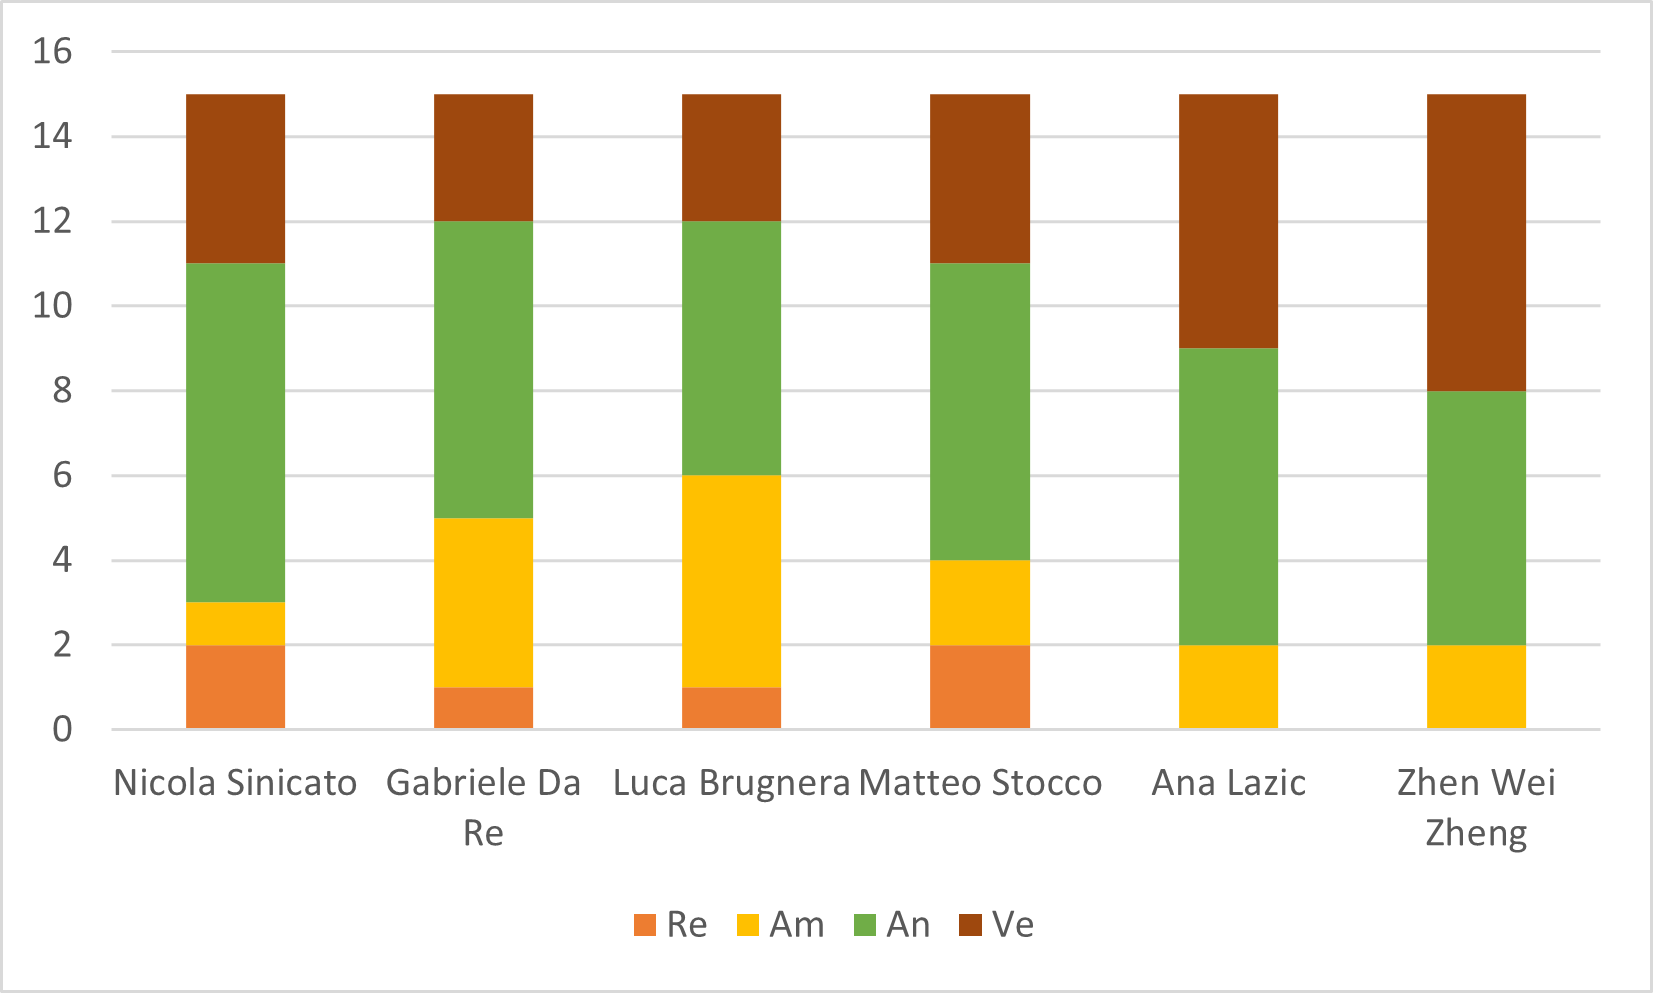
\includegraphics[scale=0.6]{img/grafi preventivo/istogrammi/analisi/periodo2.png}
    \caption{Istogramma della ripartizione delle ore del secondo periodo della fase di analisi}
\end{figure}
\begin{figure}[H]
    \centering
    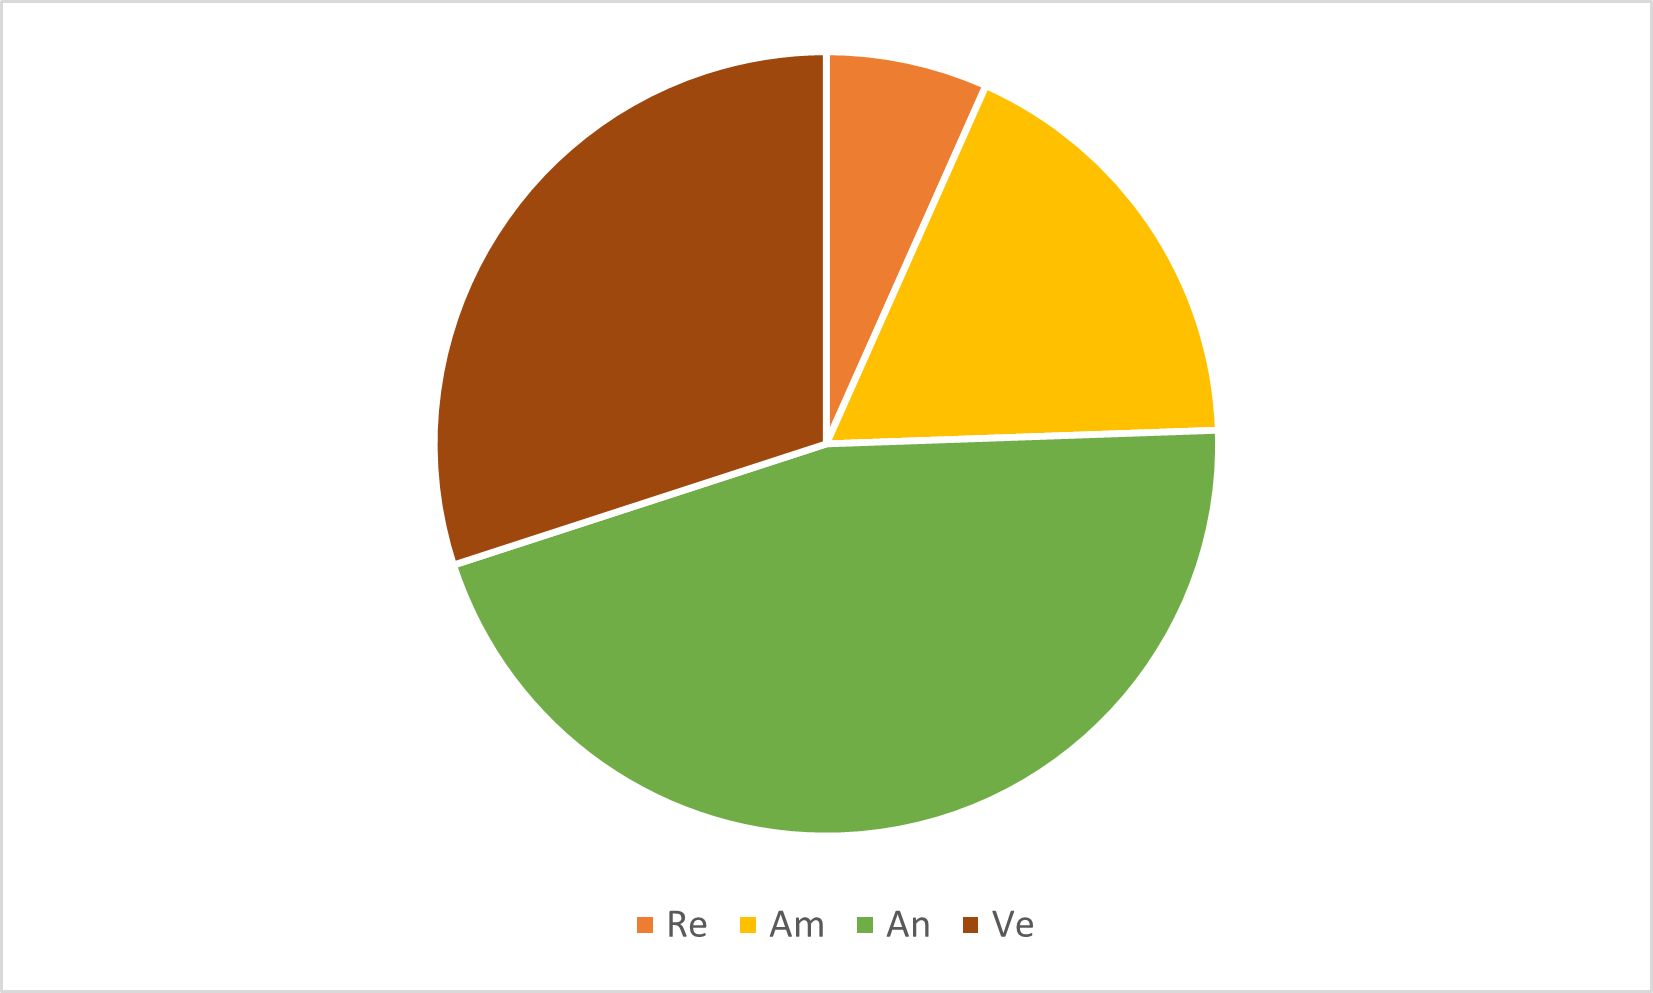
\includegraphics[scale=0.6]{img/grafi preventivo/torta/analisi/periodo2.png}
    \caption{Grafico a torta della ripartizione delle ore per ruolo nel secondo periodo della fase di analisi}
\end{figure}
\subsubsubsection{Preventivo dei costi}
La seguente tabella rappresenta le ore dedicate ad ogni ruolo e il corrispettivo costo in euro per il secondo periodo della fase di analisi:

	\setlength\extrarowheight{5pt}
	\rowcolors{2}{gray!10}{gray!40}
	\begin{tabularx}{\textwidth}{|ccc|c|}
		\hline
		\rowcolor{white}
		\textbf{Ruolo} & \textbf{Costo orario (€)} & \textbf{Ore totali} & \textbf{Costo totale (€)} \\
		\hline
		Responsabile &30&6&180 \\
		Amministratore &20&16&320 \\
		Analista &25&41&1025 \\
		Verificatore &15&27&405 \\
		Programmatore &15&0&0 \\
		Progettista &25&0&0 \\
		\hline
		Totale &-&-&1930 \\
		\hline
		\rowcolor{white}
		\caption{Prospetto del costo orario durante il secondo periodo di analisi per ruolo}
	\end{tabularx}
    \vspace{10pt}
	
%
% ----------------------------------------------------------------------------------------------------------------
\newpage
\subsubsection{Periodo 3}
% ----------------------------------------------------------------------------------------------------------------
%
\subsubsubsection{Preventivo orario}
La seguente tabella rappresenta la distribuzione oraria per ogni componente per il terzo periodo della fase di analisi:

	\setlength\extrarowheight{5pt}
	\rowcolors{2}{gray!10}{gray!40}
	\begin{tabularx}{\textwidth}{|ccccccc|c|}
		\hline
		\rowcolor{white}
		\textbf{Nome} & \textbf{Re} & \textbf{Am} & \textbf{An} & \textbf{Ve} & \textbf{Pr}& \textbf{Pt} & \textbf{Ore totali} \\
		\hline
		Nicola Sinicato &0&1&1&3&0&0&5 \\
		Gabriele Da Re &1&2&1&1&0&0&5 \\
		Luca Brugnera &0&2&1&2&0&0&5 \\
		Matteo Stocco &1&1&2&1&0&0&5 \\
		Ana Lazic &1&0&1&3&0&0&5 \\
		Zhen Wei Zheng &0&0&2&3&0&0&5 \\
		\hline
		Ore totali ruolo &3&6&8&13&0&0&30 \\
		\hline
		\rowcolor{white}
		\caption{Distribuzione oraria durante il terzo periodo di analisi per ruolo e persona}
	\end{tabularx}
	\vspace{10pt}
	
\begin{figure}[H]
    \centering
    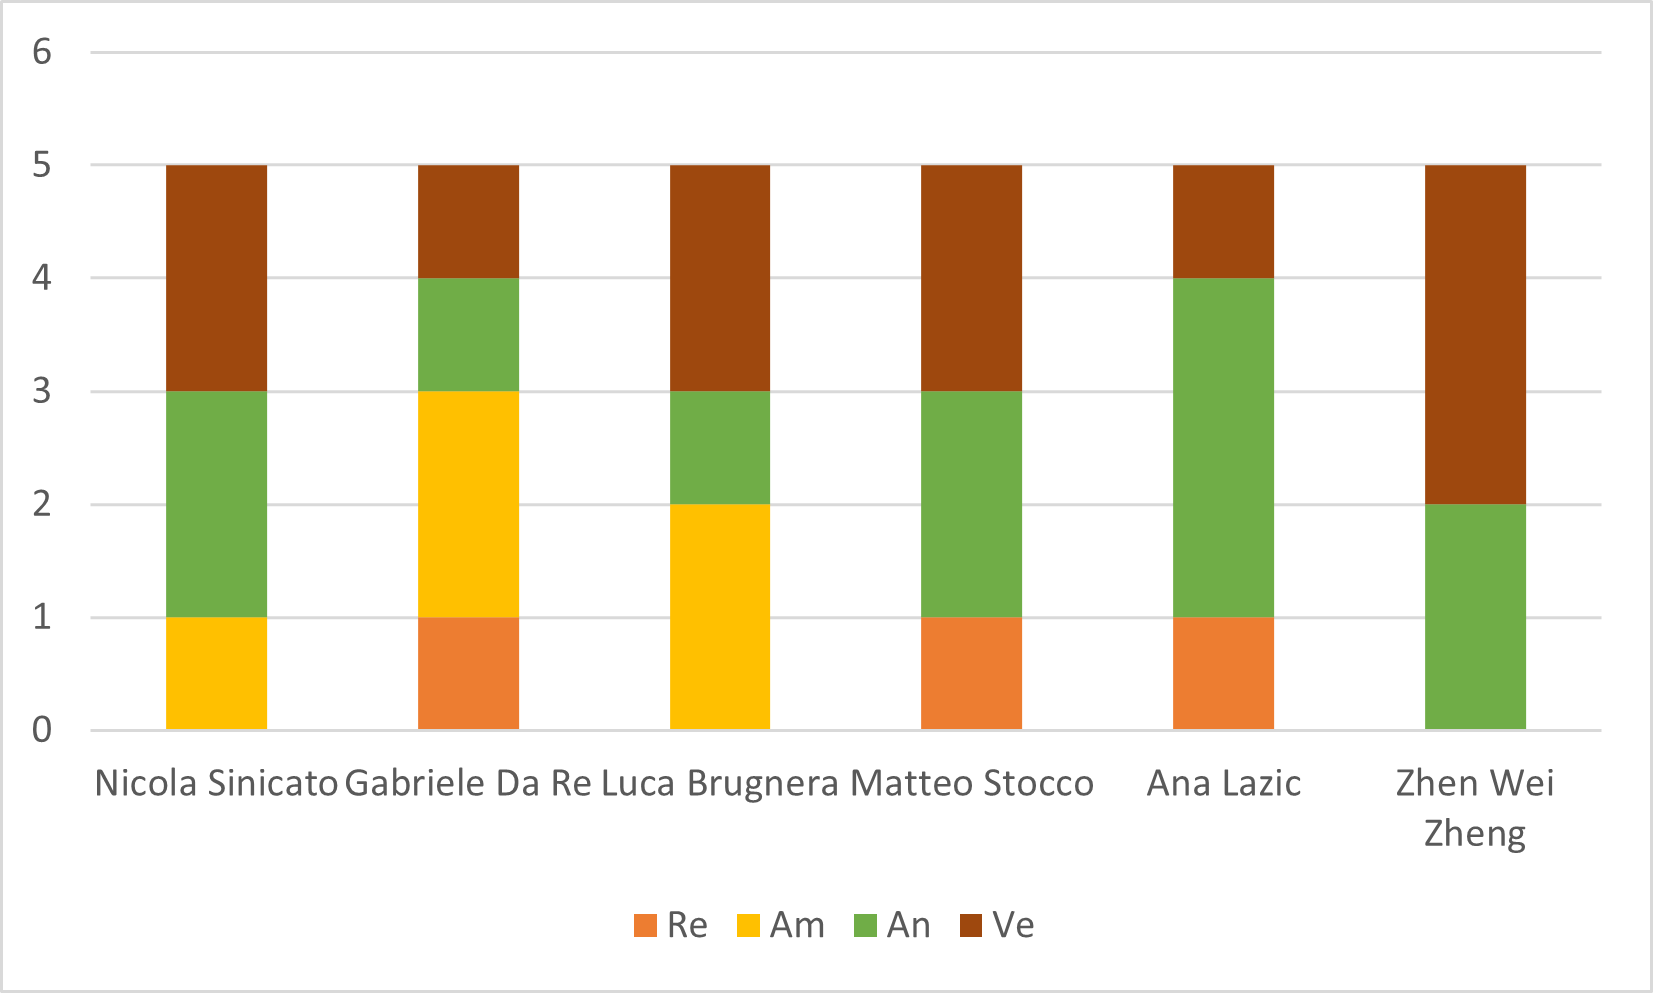
\includegraphics[scale=0.6]{img/grafi preventivo/istogrammi/analisi/periodo3.png}
    \caption{Istogramma della ripartizione delle ore del terzo periodo della fase di analisi}
\end{figure}
\begin{figure}[H]
    \centering
    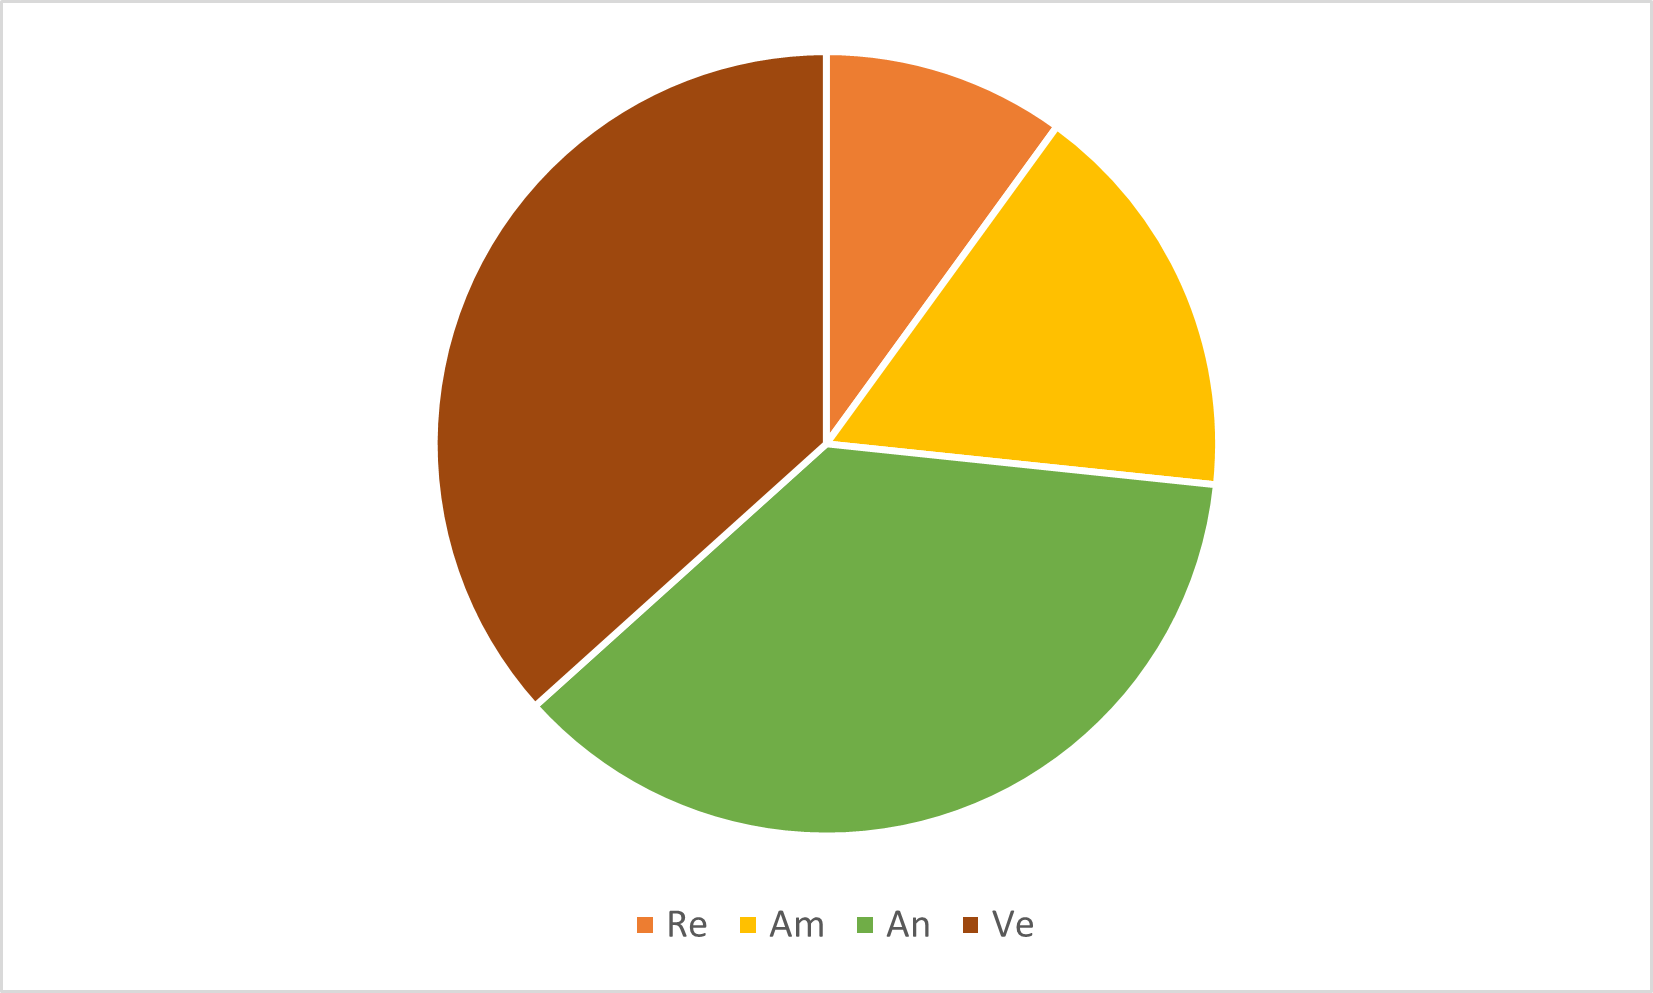
\includegraphics[scale=0.6]{img/grafi preventivo/torta/analisi/periodo3.png}
    \caption{Grafico a torta della ripartizione delle ore per ruolo nel terzo periodo della fase di analisi}
\end{figure}
\subsubsubsection{Preventivo dei costi}
La seguente tabella rappresenta le ore dedicate ad ogni ruolo e il corrispettivo costo in euro per il terzo periodo della fase di analisi:

	\setlength\extrarowheight{5pt}
	\rowcolors{2}{gray!10}{gray!40}
	\begin{tabularx}{\textwidth}{|ccc|c|}
		\hline
		\rowcolor{white}
		\textbf{Ruolo} & \textbf{Costo orario (€)} & \textbf{Ore totali} & \textbf{Costo totale (€)} \\
		\hline
		Responsabile &30&3&90 \\
		Amministratore &20&6&120 \\
		Analista &25&8&200 \\
		Verificatore &15&13&195 \\
		Programmatore &15&0&0 \\
		Progettista &25&0&0 \\
		\hline
		Totale &-&-&605 \\
		\hline
		\rowcolor{white}
		\caption{Prospetto del costo orario durante il terzo periodo di analisi per ruolo}
	\end{tabularx}
    \vspace{10pt}
	
%
% ----------------------------------------------------------------------------------------------------------------
\newpage
\subsubsection{Riepilogo della fase di analisi}
% ----------------------------------------------------------------------------------------------------------------
%
\subsubsubsection{Preventivo orario}
La seguente tabella rappresenta la distribuzione oraria per ogni componente per la fase di analisi:

	\setlength\extrarowheight{5pt}
	\rowcolors{2}{gray!10}{gray!40}
	\begin{tabularx}{\textwidth}{|ccccccc|c|}
		\hline
		\rowcolor{white}
		\textbf{Nome} & \textbf{Re} & \textbf{Am} & \textbf{An} & \textbf{Ve} & \textbf{Pr}& \textbf{Pt} & \textbf{Ore totali} \\
		\hline
		Nicola Sinicato &5&5&13&7&0&0&30 \\
		Gabriele Da Re &2&12&12&4&0&0&30 \\
		Luca Brugnera &1&13&11&5&0&0&30 \\
		Matteo Stocco &4&8&13&5&0&0&30 \\
		Ana Lazic &2&5&14&9&0&0&30 \\
		Zhen Wei Zheng &1&5&14&10&0&0&30 \\
		\hline
		Ore totali ruolo &15&48&77&40&0&0&180 \\
		\hline
		\rowcolor{white}
		\caption{Distribuzione oraria durante la fase di analisi per ruolo e persona}
	\end{tabularx}
	\vspace{10pt}
	
\begin{figure}[H]
    \centering
    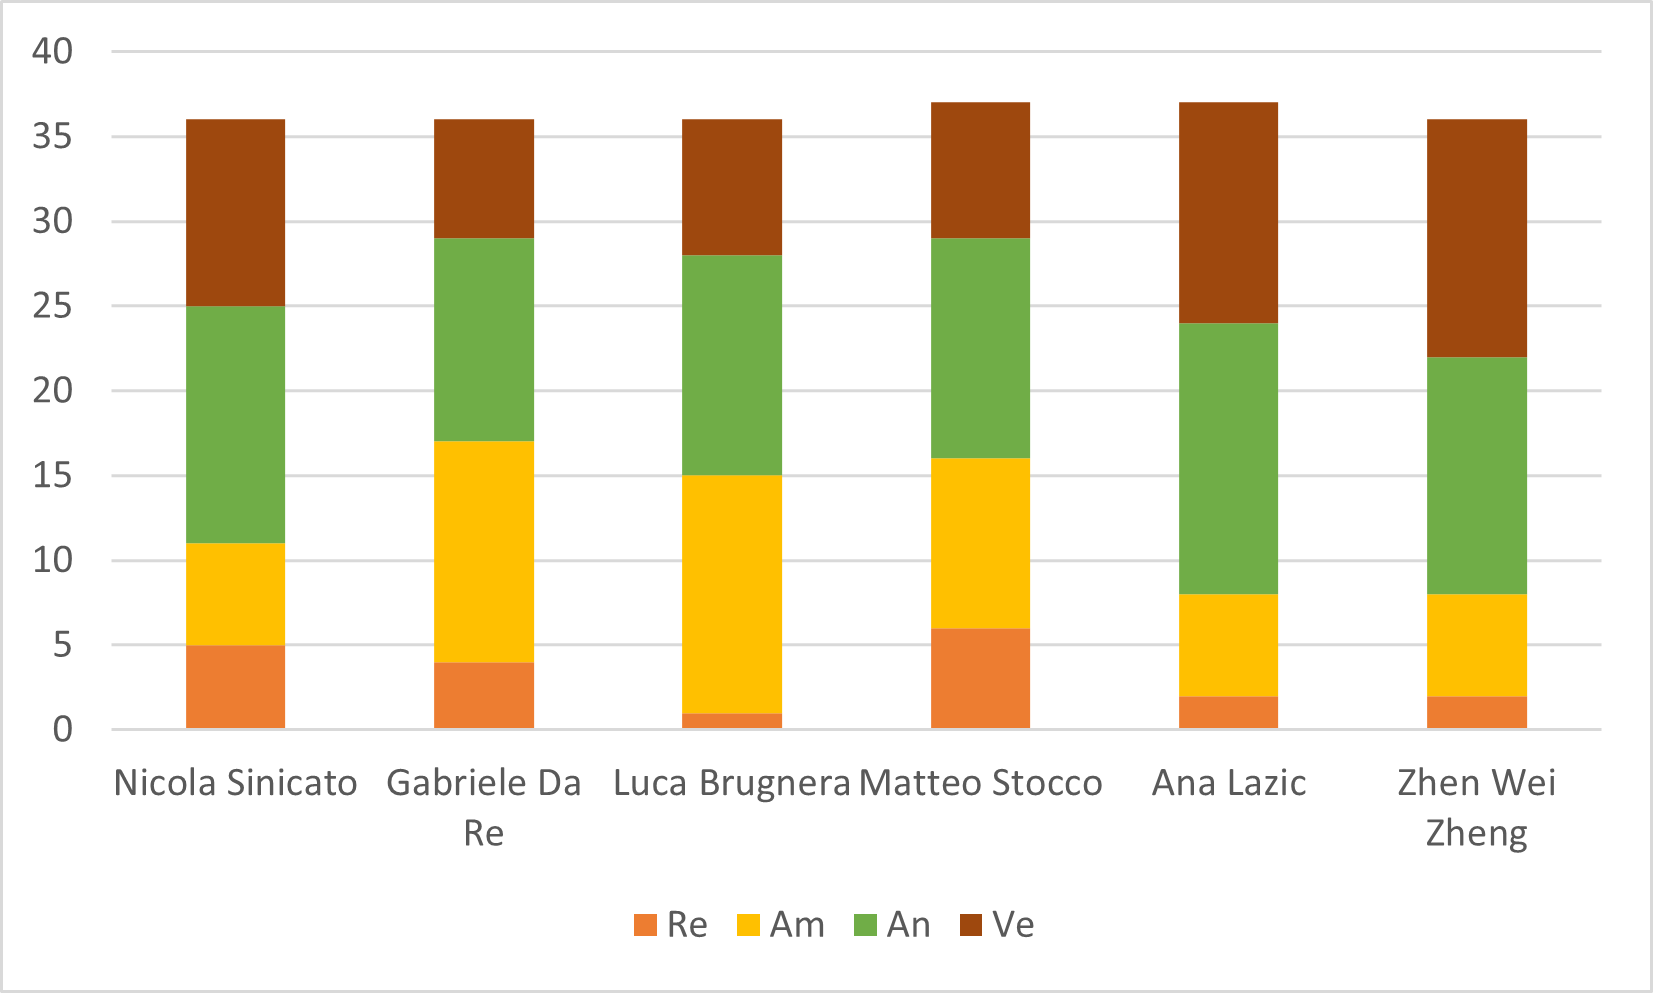
\includegraphics[scale=0.6]{img/grafi preventivo/istogrammi/analisi/complessivo.png}
    \caption{Istogramma della ripartizione delle ore della fase di analisi}
\end{figure}
\begin{figure}[H]
    \centering
    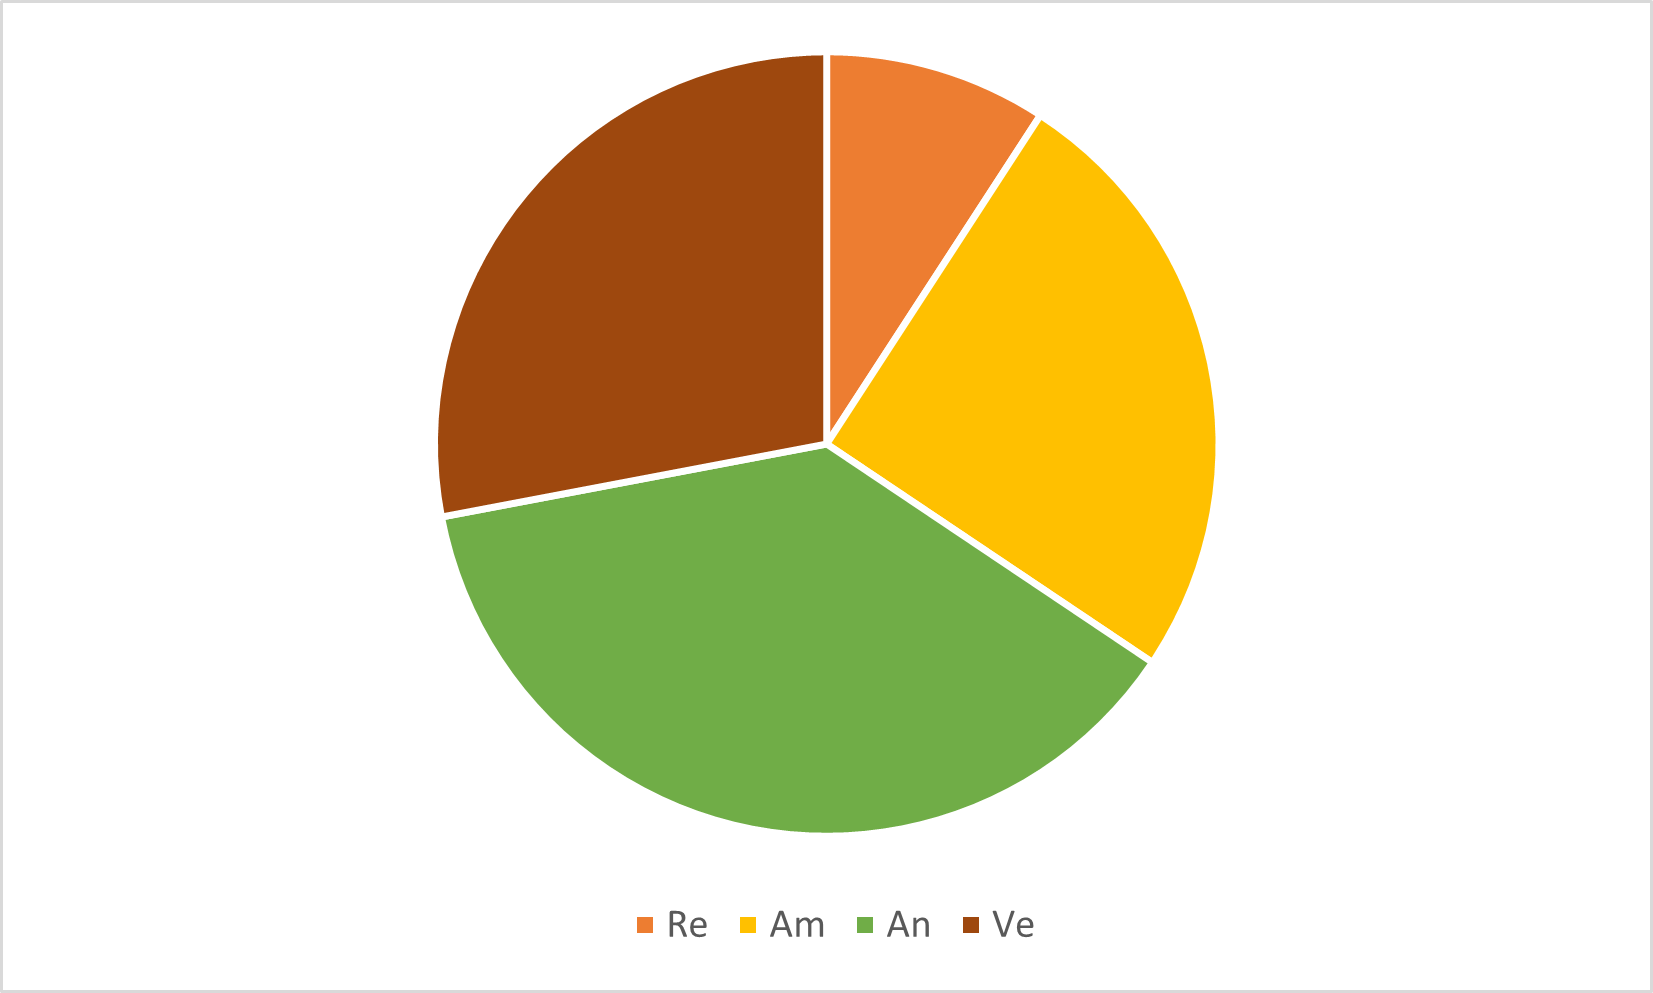
\includegraphics[scale=0.6]{img/grafi preventivo/torta/analisi/complessivo.png}
    \caption{Grafico a torta della ripartizione delle ore per ruolo nella fase di analisi}
\end{figure}
\subsubsubsection{Preventivo dei costi}
La seguente tabella rappresenta le ore dedicate ad ogni ruolo e il corrispettivo costo in euro per la fase di analisi:

	\setlength\extrarowheight{5pt}
	\rowcolors{2}{gray!10}{gray!40}
	\begin{tabularx}{\textwidth}{|ccc|c|}
		\hline
		\rowcolor{white}
		\textbf{Ruolo} & \textbf{Costo orario (€)} & \textbf{Ore totali} & \textbf{Costo totale (€)} \\
		\hline
		Responsabile &30&15&450 \\
		Amministratore &20&48&960 \\
		Analista &25&77&1925 \\
		Verificatore &15&40&600 \\
		Programmatore &15&0&0 \\
		Progettista &25&0&0 \\
		\hline
		Totale &-&-&3935 \\
		\hline
		\rowcolor{white}
		\caption{Prospetto del costo orario durante la fase di analisi per ruolo}
	\end{tabularx}
    \vspace{10pt}
	
% ----------------------------------------------------------------------------------------------------------------
%
\newpage
\subsection{Produzione del Proof of Concept}

% ----------------------------------------------------------------------------------------------------------------
\subsubsection{Periodo 1}
% ----------------------------------------------------------------------------------------------------------------
%
\subsubsubsection{Preventivo orario}
La seguente tabella rappresenta la distribuzione oraria per ogni componente per il primo periodo della fase di produzione del Proof of Concept:

	\setlength\extrarowheight{5pt}
	\rowcolors{2}{gray!10}{gray!40}
	\begin{tabularx}{\textwidth}{|ccccccc|c|}
		\hline
		\rowcolor{white}
		\textbf{Nome} & \textbf{Re} & \textbf{Am} & \textbf{An} & \textbf{Ve} & \textbf{Pr}& \textbf{Pt} & \textbf{Ore totali} \\
		\hline
		Nicola Sinicato &1&1&0&0&1&1&4 \\
		Gabriele Da Re &0&1&0&0&1&2&4 \\
		Luca Brugnera &1&0&1&1&0&1&4 \\
		Matteo Stocco &0&0&1&1&1&1&4 \\
		Ana Lazic &1&0&1&0&1&1&4 \\
		Zhen Wei Zheng &1&1&1&0&0&1&4 \\
		\hline
		Ore totali ruolo &4&3&4&2&4&7&24 \\
		\hline
		\rowcolor{white}
		\caption{Distribuzione oraria durante  il primo periodo di produzione del Proof of Concept per ruolo e persona}
	\end{tabularx}
	\vspace{10pt}
	
\begin{figure}[H]
    \centering
    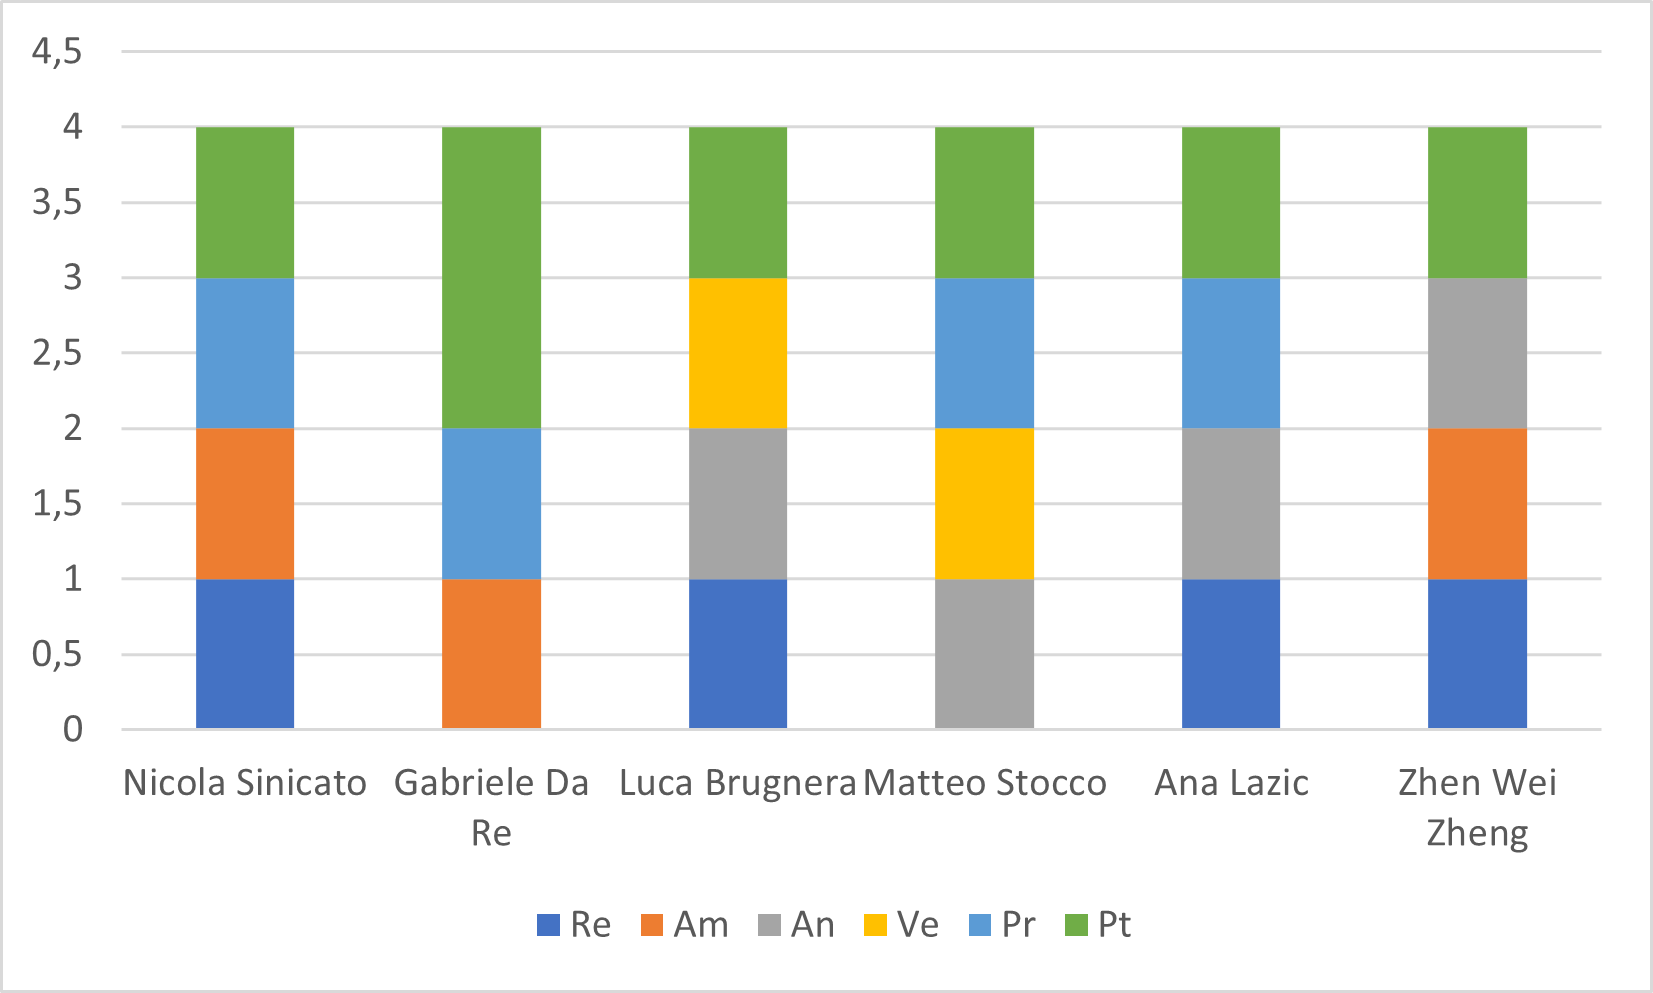
\includegraphics[scale=0.6]{img/grafi preventivo/istogrammi/proof/periodo1.png}
    \caption{Istogramma della ripartizione delle ore del primo periodo della fase di produzione del Proof of Concept}
\end{figure}
\begin{figure}[H]
    \centering
    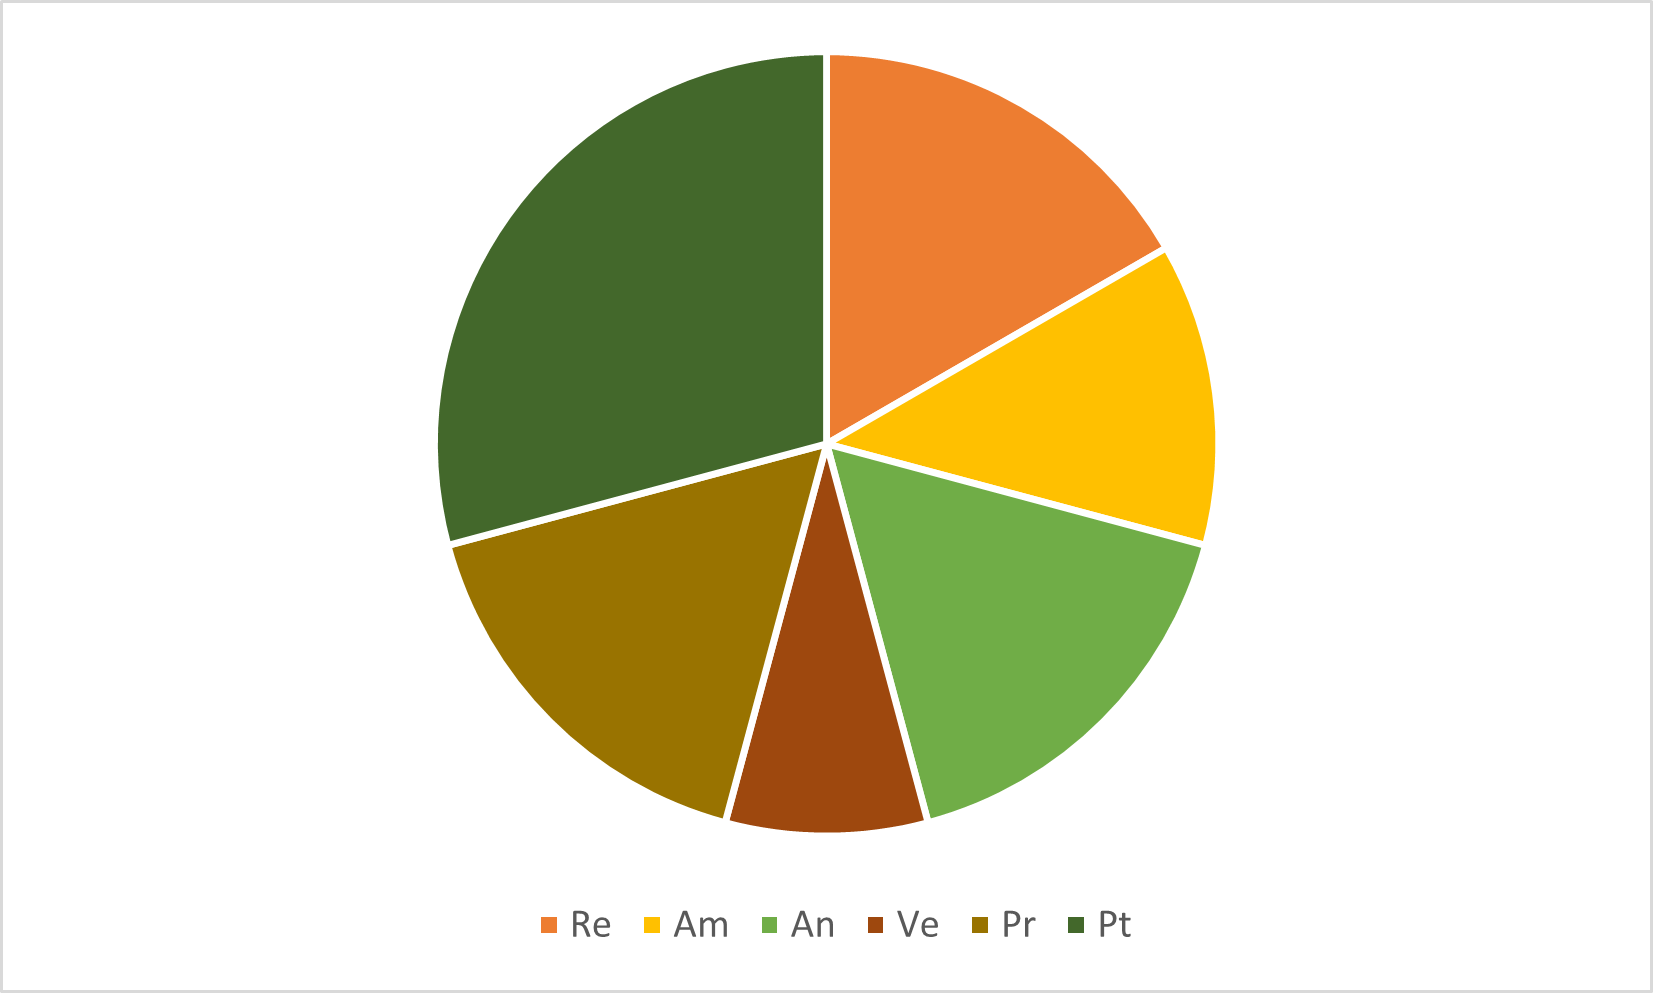
\includegraphics[scale=0.6]{img/grafi preventivo/torta/proof/periodo1.png}
    \caption{Grafico a torta della ripartizione delle ore per ruolo nel primo periodo della fase di produzione del Proof of Concept}
\end{figure}
\subsubsubsection{Preventivo dei costi}
La seguente tabella rappresenta le ore dedicate ad ogni ruolo e il corrispettivo costo in euro per il primo periodo della fase di produzione del Proof of Concept:

	\setlength\extrarowheight{5pt}
	\rowcolors{2}{gray!10}{gray!40}
	\begin{tabularx}{\textwidth}{|ccc|c|}
		\hline
		\rowcolor{white}
		\textbf{Ruolo} & \textbf{Costo orario (€)} & \textbf{Ore totali} & \textbf{Costo totale (€)} \\
		\hline
		Responsabile &30&4&120 \\
		Amministratore &20&3&60 \\
		Analista &25&4&100 \\
		Verificatore &15&2&30 \\
		Programmatore &15&4&60 \\
		Progettista &25&7&175 \\
		\hline
		Totale &-&-&545 \\
		\hline
		\rowcolor{white}
		\caption{Prospetto del costo orario durante  il primo periodo di produzione del Proof of Concept per ruolo}
	\end{tabularx}
    \vspace{10pt}
	
% ----------------------------------------------------------------------------------------------------------------
\newpage
\subsubsection{Periodo 2}
% ----------------------------------------------------------------------------------------------------------------
%
\subsubsubsection{Preventivo orario}
La seguente tabella rappresenta la distribuzione oraria per ogni componente per il secondo periodo della fase di produzione del Proof of Concept:

	\setlength\extrarowheight{5pt}
	\rowcolors{2}{gray!10}{gray!40}
	\begin{tabularx}{\textwidth}{|ccccccc|c|}
		\hline
		\rowcolor{white}
		\textbf{Nome} & \textbf{Re} & \textbf{Am} & \textbf{An} & \textbf{Ve} & \textbf{Pr}& \textbf{Pt} & \textbf{Ore totali} \\
		\hline
		Nicola Sinicato &0&1&0&1&4&0&6 \\
		Gabriele Da Re &2&0&0&0&1&3&6 \\
		Luca Brugnera &0&0&2&1&3&0&6 \\
		Matteo Stocco &0&1&0&3&2&0&6 \\
		Ana Lazic &0&1&0&0&3&2&6 \\
		Zhen Wei Zheng &1&0&0&2&0&3&6 \\
		\hline
		Ore totali ruolo &3&3&2&7&13&8&36 \\
		\hline
		\rowcolor{white}
		\caption{Distribuzione oraria durante il secondo periodo di produzione del Proof of Concept per ruolo e persona}
	\end{tabularx}
	\vspace{10pt}
	
\begin{figure}[H]
    \centering
    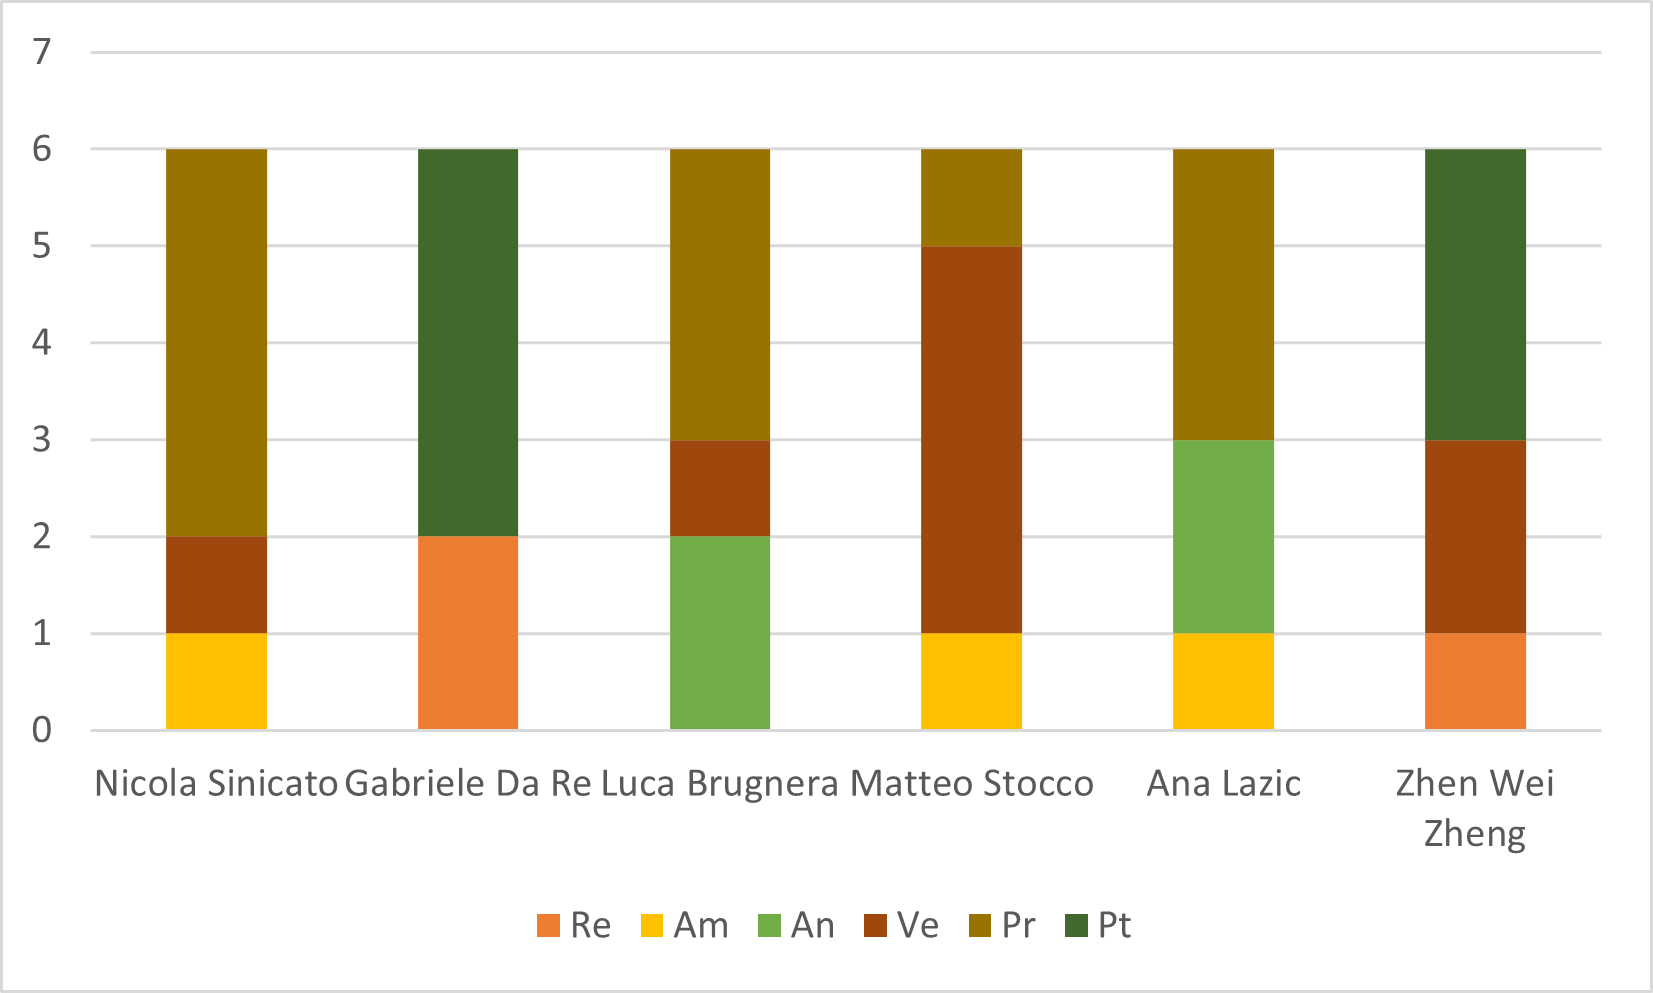
\includegraphics[scale=0.6]{img/grafi preventivo/istogrammi/proof/periodo2.png}
    \caption{Istogramma della ripartizione delle ore del secondo periodo della fase di produzione del Proof of Concept}
\end{figure}
\begin{figure}[H]
    \centering
    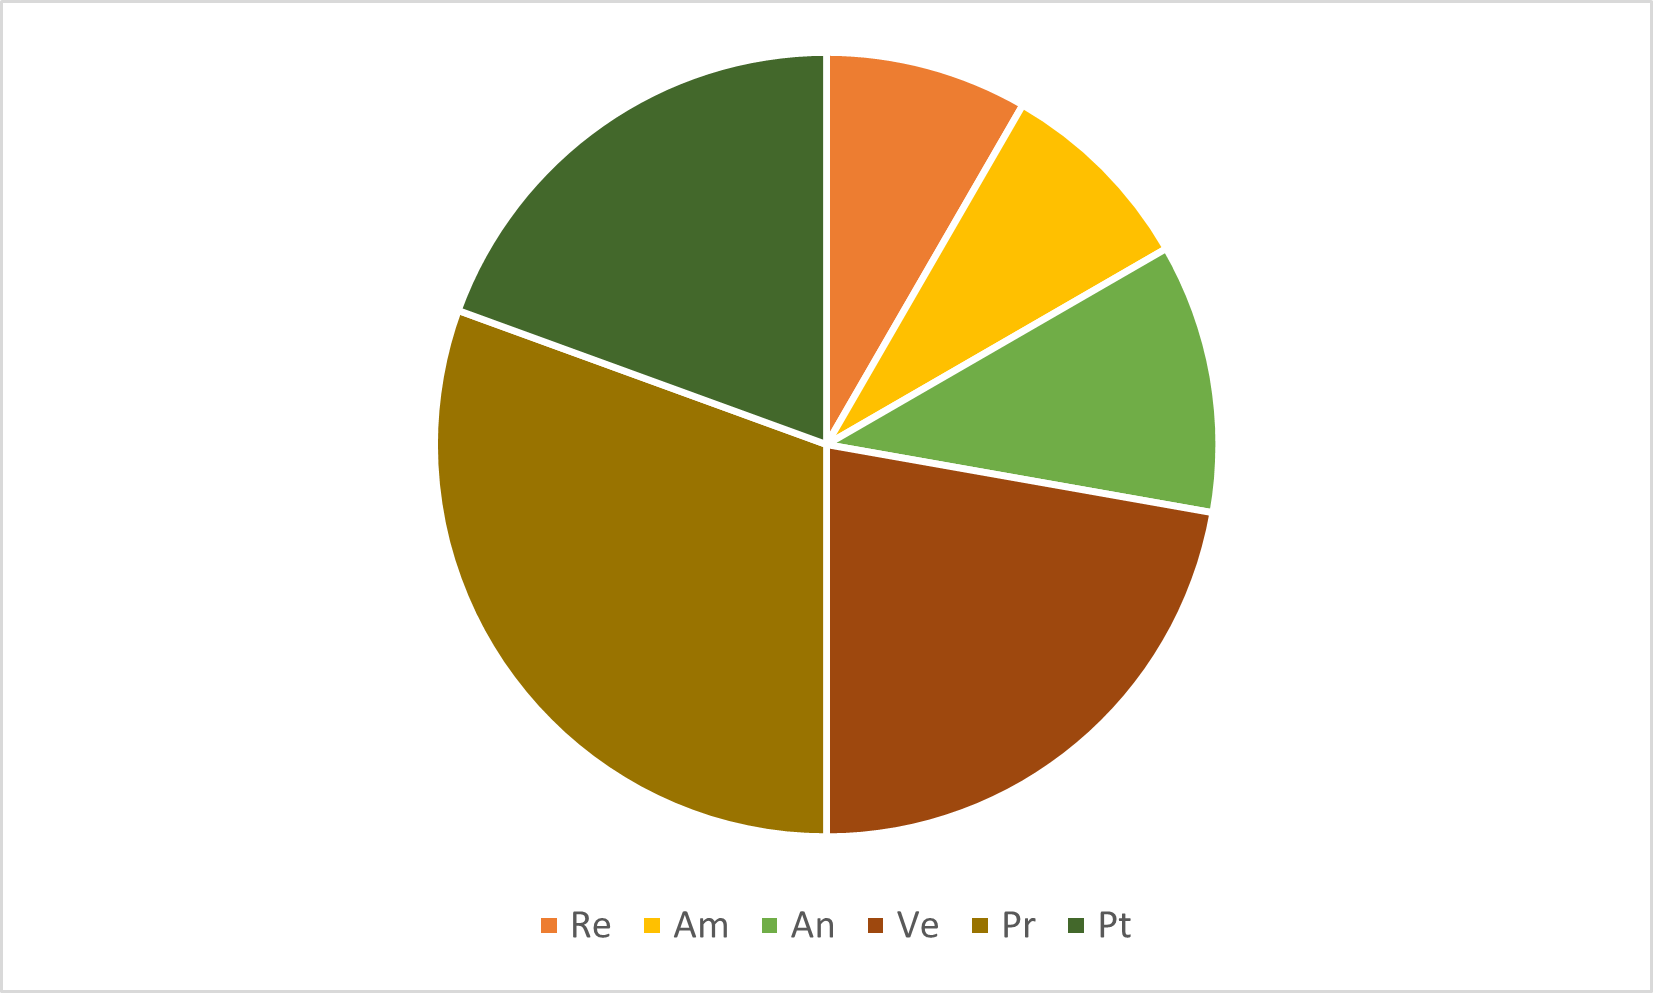
\includegraphics[scale=0.6]{img/grafi preventivo/torta/proof/periodo2.png}
    \caption{Grafico a torta della ripartizione delle ore per ruolo nel secondo periodo della fase di produzione del Proof of Concept}
\end{figure}
\subsubsubsection{Preventivo dei costi}
La seguente tabella rappresenta le ore dedicate ad ogni ruolo e il corrispettivo costo in euro per il secondo periodo della fase di produzione del Proof of Concept:

	\setlength\extrarowheight{5pt}
	\rowcolors{2}{gray!10}{gray!40}
	\begin{tabularx}{\textwidth}{|ccc|c|}
		\hline
		\rowcolor{white}
		\textbf{Ruolo} & \textbf{Costo orario (€)} & \textbf{Ore totali} & \textbf{Costo totale (€)} \\
		\hline
		Responsabile &30&3&90 \\
		Amministratore &20&3&60 \\
		Analista &25&2&50 \\
		Verificatore &15&7&105 \\
		Programmatore &15&13&195 \\
		Progettista &25&8&200 \\
		\hline
		Totale &-&-&700 \\
		\hline
		\rowcolor{white}
		\caption{Prospetto del costo orario durante  il secondo periodo di produzione del Proof of Concept per ruolo}
	\end{tabularx}
    \vspace{10pt}
	
% ----------------------------------------------------------------------------------------------------------------
\newpage
\subsubsection{Riepilogo della fase di produzione del Proof of Concept}
% ----------------------------------------------------------------------------------------------------------------
%
\subsubsubsection{Preventivo orario}
La seguente tabella rappresenta la distribuzione oraria per ogni componente la fase di produzione del Proof of Concept:

	\setlength\extrarowheight{5pt}
	\rowcolors{2}{gray!10}{gray!40}
	\begin{tabularx}{\textwidth}{|ccccccc|c|}
		\hline
		\rowcolor{white}
		\textbf{Nome} & \textbf{Re} & \textbf{Am} & \textbf{An} & \textbf{Ve} & \textbf{Pr}& \textbf{Pt} & \textbf{Ore totali} \\
		\hline
		Nicola Sinicato &1&2&0&1&5&1&10 \\
		Gabriele Da Re &2&1&0&0&2&5&10 \\
		Luca Brugnera &1&0&3&2&3&1&10 \\
		Matteo Stocco &0&1&1&4&3&1&10 \\
		Ana Lazic &1&1&1&0&4&3&10 \\
		Zhen Wei Zheng &2&1&1&2&0&4&10 \\
		\hline
		Ore totali ruolo &7&6&6&9&17&15&60 \\
		\hline
		\rowcolor{white}
		\caption{Distribuzione oraria durante la fase di produzione del Proof of Concept per ruolo e persona}
	\end{tabularx}
	\vspace{10pt}
	
\begin{figure}[H]
    \centering
    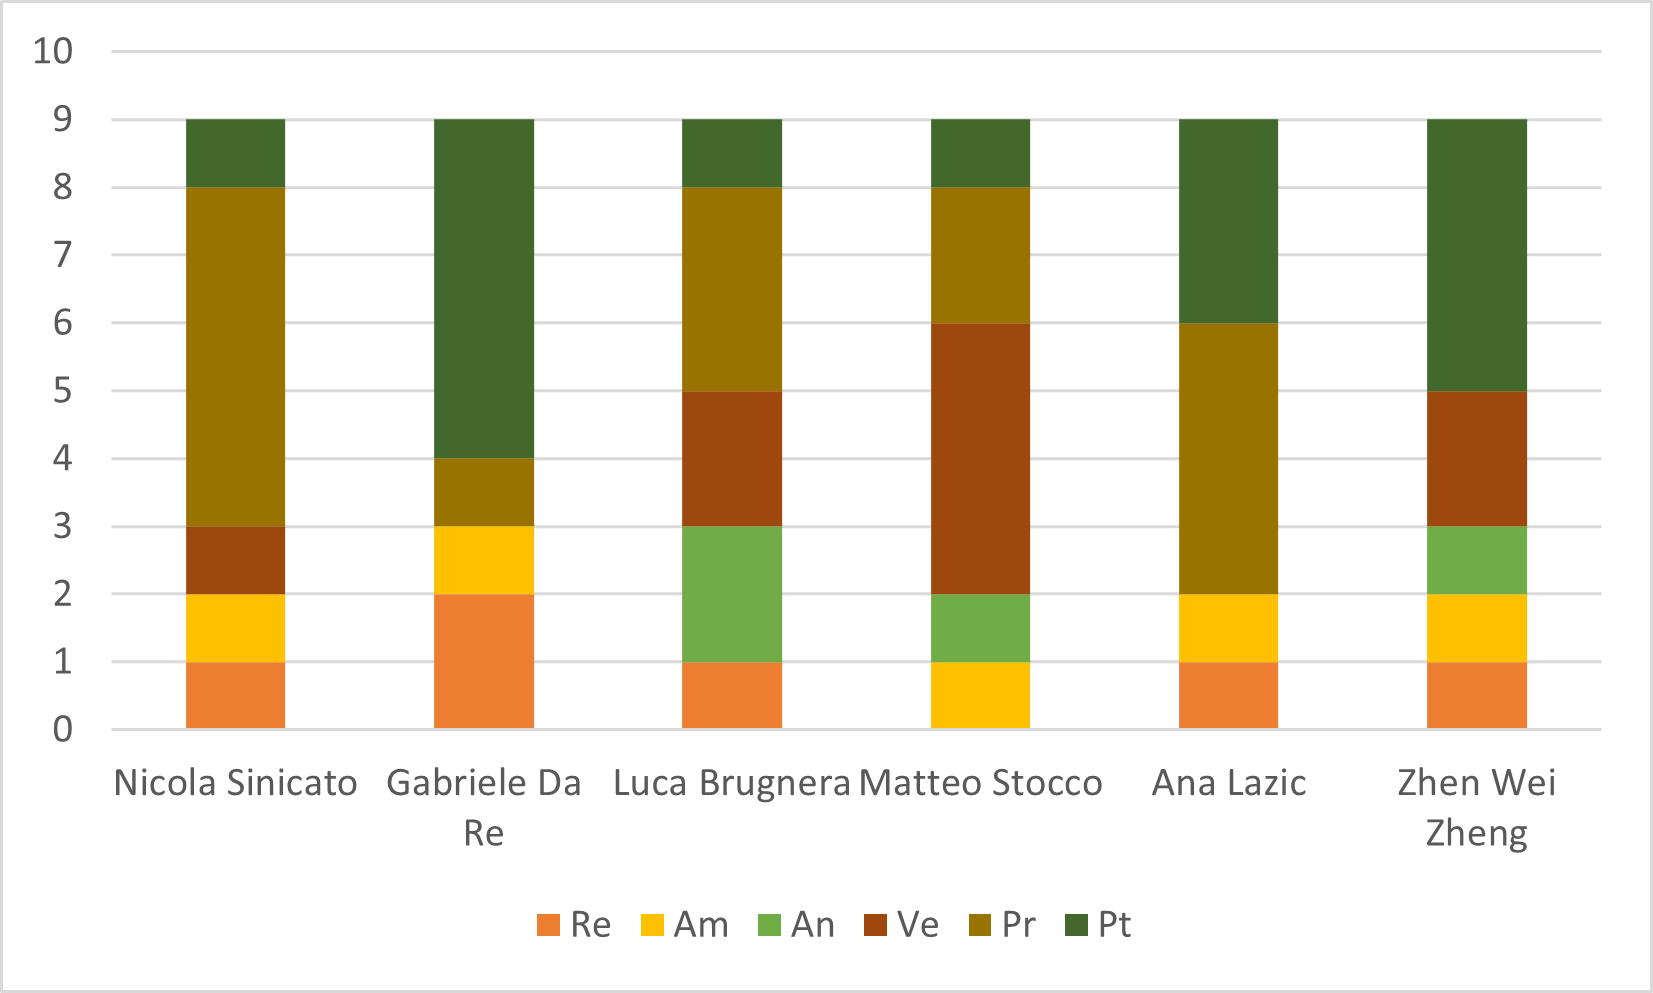
\includegraphics[scale=0.6]{img/grafi preventivo/istogrammi/proof/complessivo.png}
    \caption{Istogramma della ripartizione delle ore della fase di produzione del Proof of Concept}
\end{figure}
\begin{figure}[H]
    \centering
    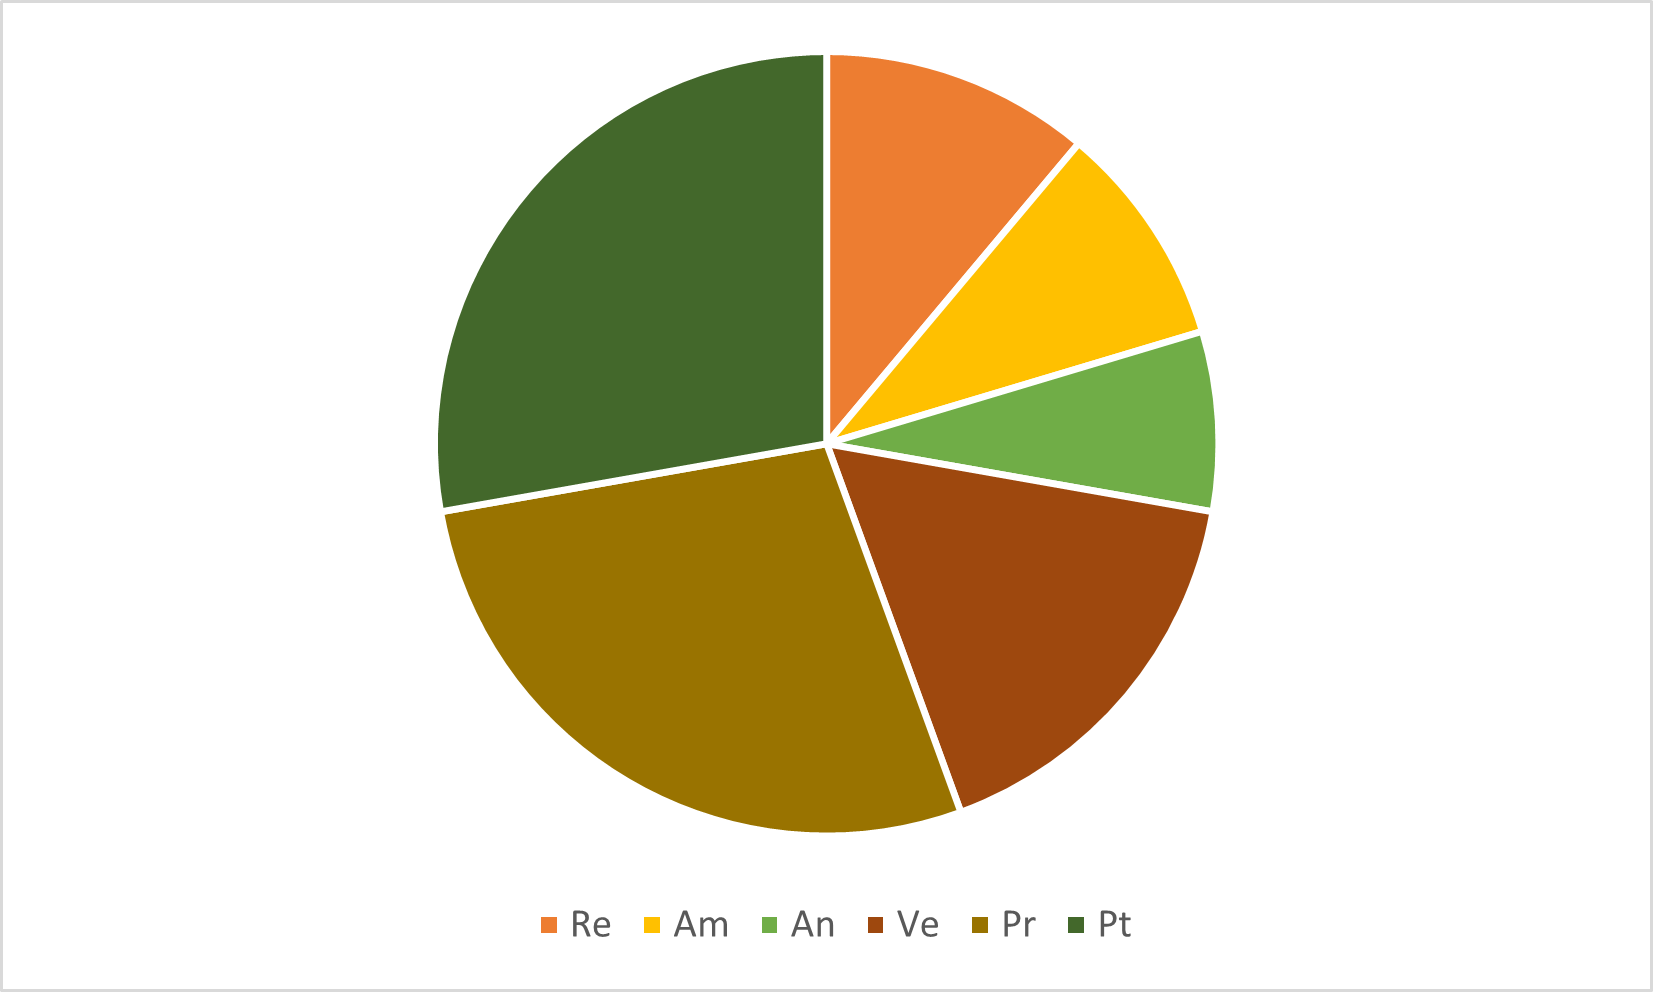
\includegraphics[scale=0.6]{img/grafi preventivo/torta/proof/complessivo.png}
    \caption{Grafico a torta della ripartizione delle ore per ruolo nella fase di produzione del Proof of Concept}
\end{figure}
\subsubsubsection{Preventivo dei costi}
La seguente tabella rappresenta le ore dedicate ad ogni ruolo e il corrispettivo costo in euro per la fase di produzione del Proof of Concept:

	\setlength\extrarowheight{5pt}
	\rowcolors{2}{gray!10}{gray!40}
	\begin{tabularx}{\textwidth}{|ccc|c|}
		\hline
		\rowcolor{white}
		\textbf{Ruolo} & \textbf{Costo orario (€)} & \textbf{Ore totali} & \textbf{Costo totale (€)} \\
		\hline
		Responsabile &30&7&210 \\
		Amministratore &20&6&120 \\
		Analista &25&6&150 \\
		Verificatore &15&9&135 \\
		Programmatore &15&17&255 \\
		Progettista &25&15&375 \\
		\hline
		Totale &-&-&1245 \\
		\hline
		\rowcolor{white}
		\caption{Prospetto del costo orario durante la fase di produzione del Proof of Concept per ruolo}
	\end{tabularx}
    \vspace{10pt}
	
% ----------------------------------------------------------------------------------------------------------------
%
\newpage
\subsection{Progettazione architetturale}

% ----------------------------------------------------------------------------------------------------------------
\subsubsection{Periodo 1}
% ----------------------------------------------------------------------------------------------------------------
%
\subsubsubsection{Preventivo orario}
La seguente tabella rappresenta la distribuzione oraria per ogni componente per il primo periodo della fase di progettazione architetturale:

	\setlength\extrarowheight{5pt}
	\rowcolors{2}{gray!10}{gray!40}
	\begin{tabularx}{\textwidth}{|ccccccc|c|}
		\hline
		\rowcolor{white}
		\textbf{Nome} & \textbf{Re} & \textbf{Am} & \textbf{An} & \textbf{Ve} & \textbf{Pr}& \textbf{Pt} & \textbf{Ore totali} \\
		\hline
		Nicola Sinicato &1&1&1&0&0&1&4 \\
		Gabriele Da Re &0&0&0&2&0&2&4 \\
		Luca Brugnera &1&1&1&0&0&1&4 \\
		Matteo Stocco &0&1&0&2&0&1&4 \\
		Ana Lazic &0&1&1&0&0&2&4 \\
		Zhen Wei Zheng &1&0&0&1&0&2&4 \\
		\hline
		Ore totali ruolo &3&4&3&5&0&9&24 \\
		\hline
		\rowcolor{white}
		\caption{Distribuzione oraria durante  il primo periodo di progettazione architetturale per ruolo e persona}
	\end{tabularx}
	\vspace{10pt}
	
\begin{figure}[H]
    \centering
    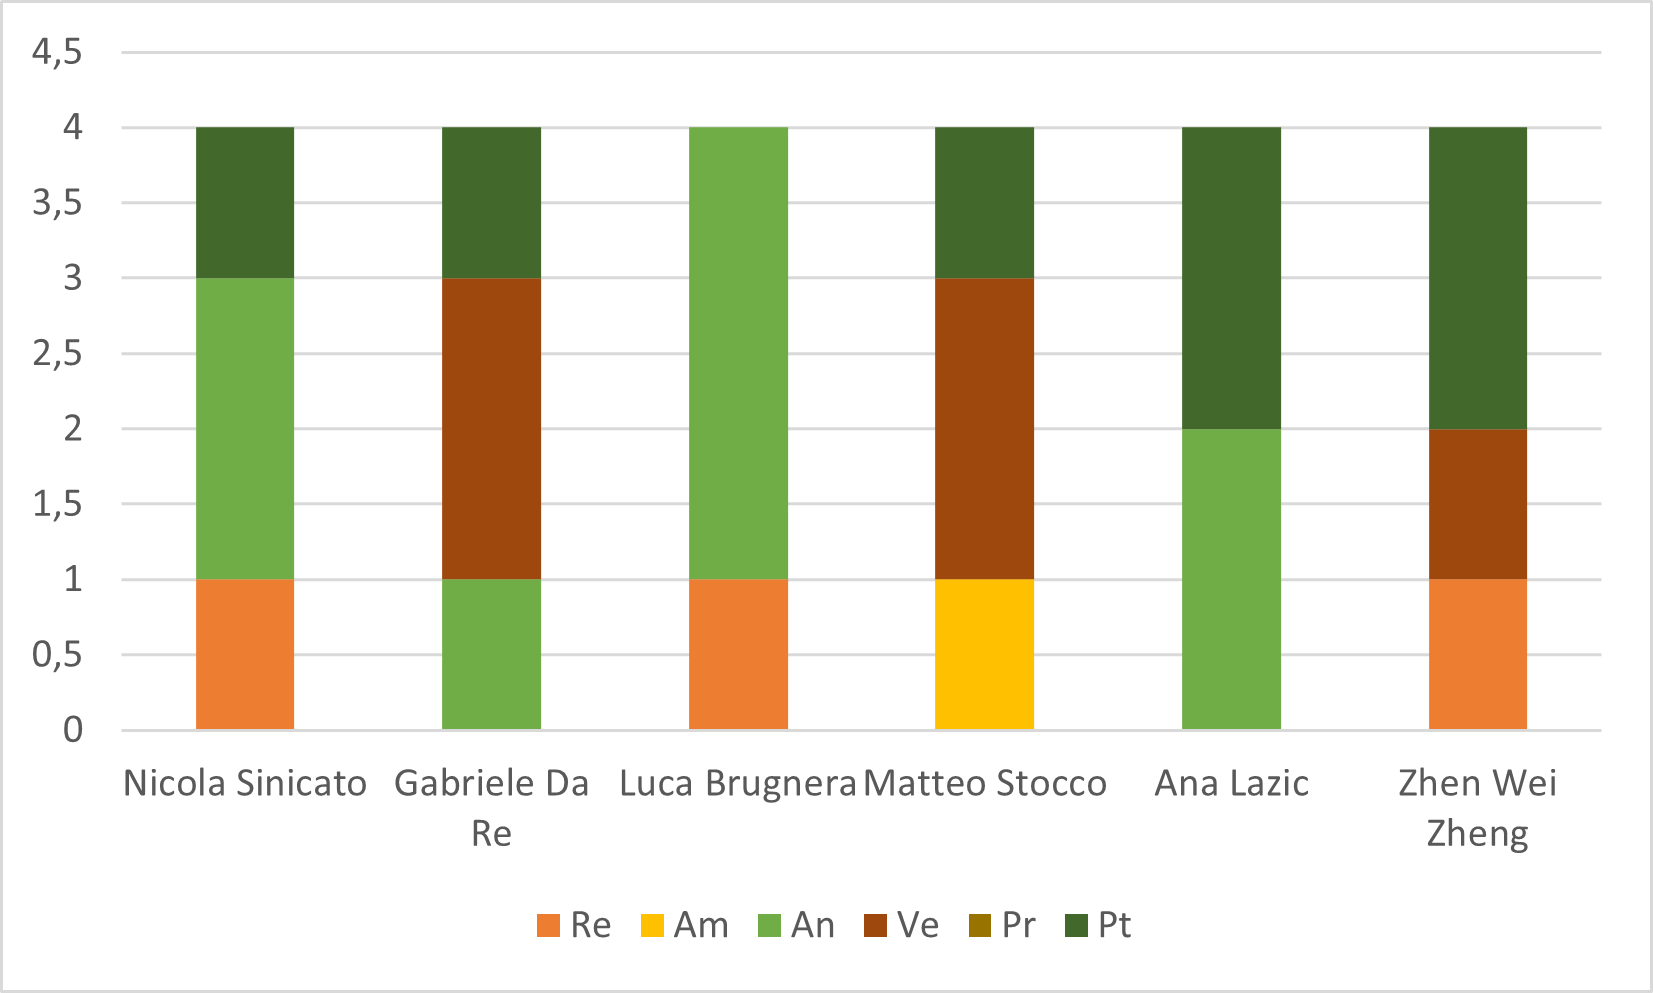
\includegraphics[scale=0.6]{img/grafi preventivo/istogrammi/architetturale/periodo1.png}
    \caption{Istogramma della ripartizione delle ore del primo periodo della fase di progettazione architetturale}
\end{figure}
\begin{figure}[H]
    \centering
    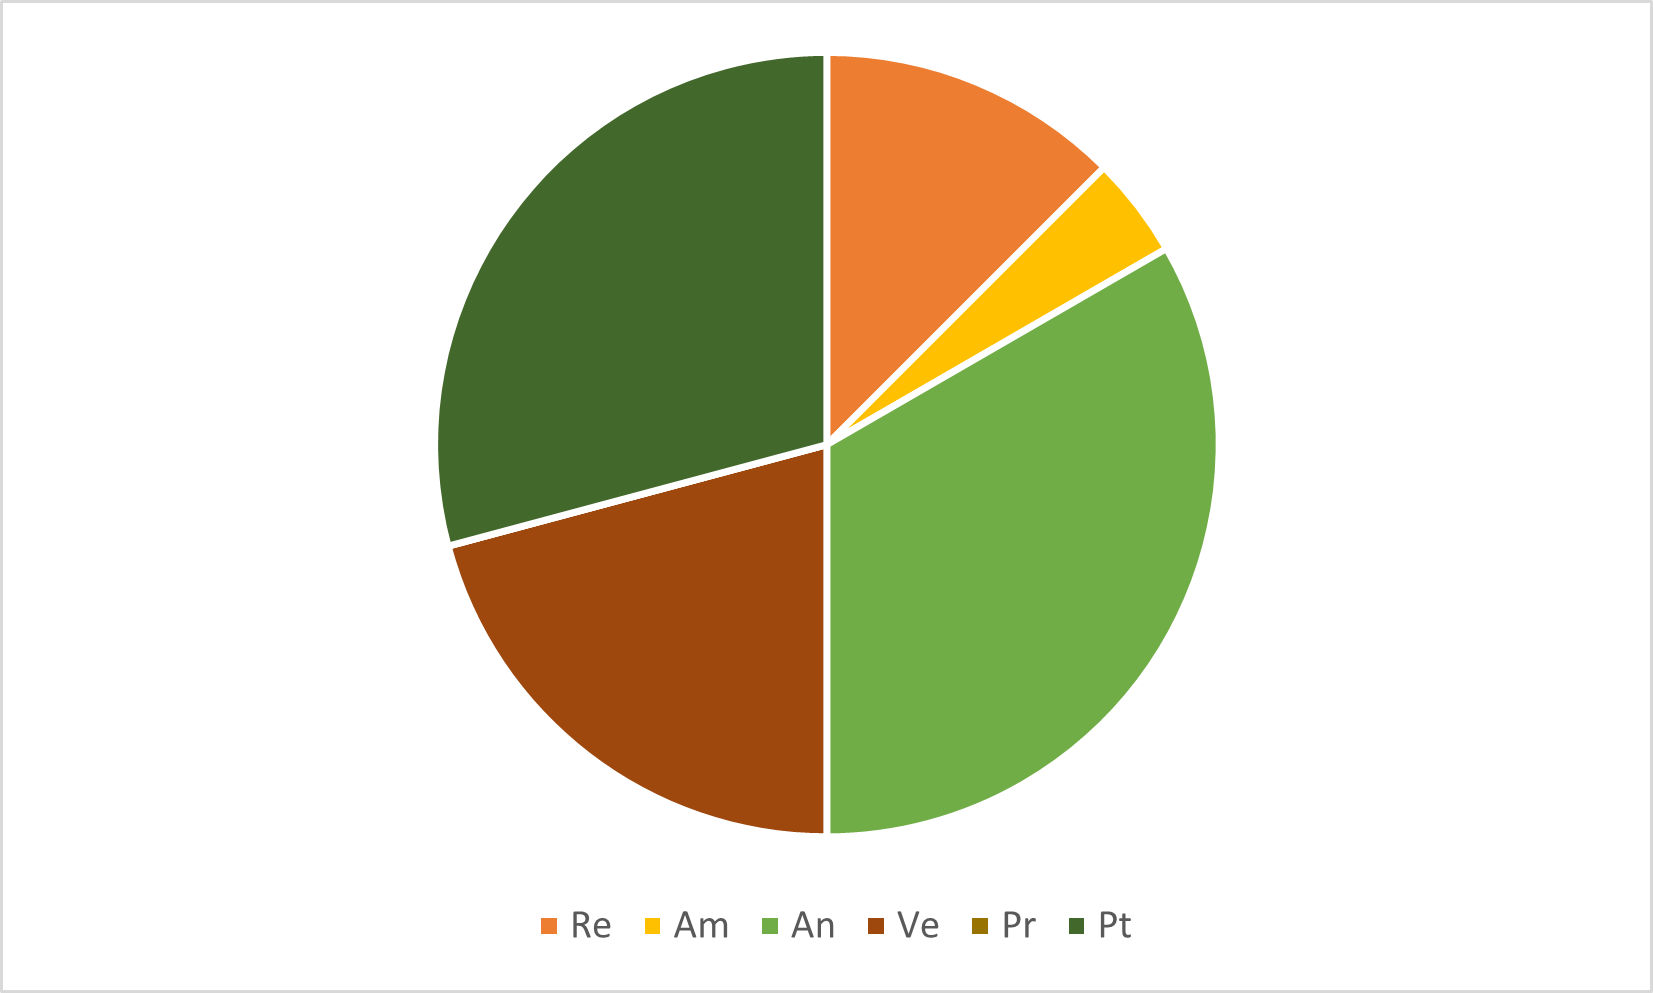
\includegraphics[scale=0.6]{img/grafi preventivo/torta/architetturale/periodo1.png}
    \caption{Grafico a torta della ripartizione delle ore per ruolo nel primo periodo della fase di progettazione architetturale}
\end{figure}
\subsubsubsection{Preventivo dei costi}
La seguente tabella rappresenta le ore dedicate ad ogni ruolo e il corrispettivo costo in euro per il primo periodo della fase di progettazione architetturale:

	\setlength\extrarowheight{5pt}
	\rowcolors{2}{gray!10}{gray!40}
	\begin{tabularx}{\textwidth}{|ccc|c|}
		\hline
		\rowcolor{white}
		\textbf{Ruolo} & \textbf{Costo orario (€)} & \textbf{Ore totali} & \textbf{Costo totale (€)} \\
		\hline
		Responsabile &30&3&90 \\
		Amministratore &20&4&80 \\
		Analista &25&3&75 \\
		Verificatore &15&5&75 \\
		Programmatore &15&0&0 \\
		Progettista &25&9&225 \\
		\hline
		Totale &-&-&545 \\
		\hline
		\rowcolor{white}
		\caption{Prospetto del costo orario durante  il primo periodo di progettazione architetturale per ruolo}
	\end{tabularx}
    \vspace{10pt}
	
% ----------------------------------------------------------------------------------------------------------------
\newpage
\subsubsection{Periodo 2}
% ----------------------------------------------------------------------------------------------------------------
%
\subsubsubsection{Preventivo orario}
La seguente tabella rappresenta la distribuzione oraria per ogni componente per il secondo periodo di fase di progettazione architetturale:

	\setlength\extrarowheight{5pt}
	\rowcolors{2}{gray!10}{gray!40}
	\begin{tabularx}{\textwidth}{|ccccccc|c|}
		\hline
		\rowcolor{white}
		\textbf{Nome} & \textbf{Re} & \textbf{Am} & \textbf{An} & \textbf{Ve} & \textbf{Pr}& \textbf{Pt} & \textbf{Ore totali} \\
		\hline
		Nicola Sinicato &0&1&0&0&0&8&9 \\
		Gabriele Da Re &1&1&0&2&0&5&9 \\
		Luca Brugnera &0&1&0&0&0&8&9 \\
		Matteo Stocco &1&0&0&2&0&6&9 \\
		Ana Lazic &1&0&0&1&0&7&9 \\
		Zhen Wei Zheng &0&1&0&1&0&7&9 \\
		\hline
		Ore totali ruolo &3&4&0&6&0&41&54 \\
		\hline
		\rowcolor{white}
		\caption{Distribuzione oraria durante il secondo periodo di progettazione architetturale per ruolo e persona}
	\end{tabularx}
	\vspace{10pt}
	
\begin{figure}[H]
    \centering
    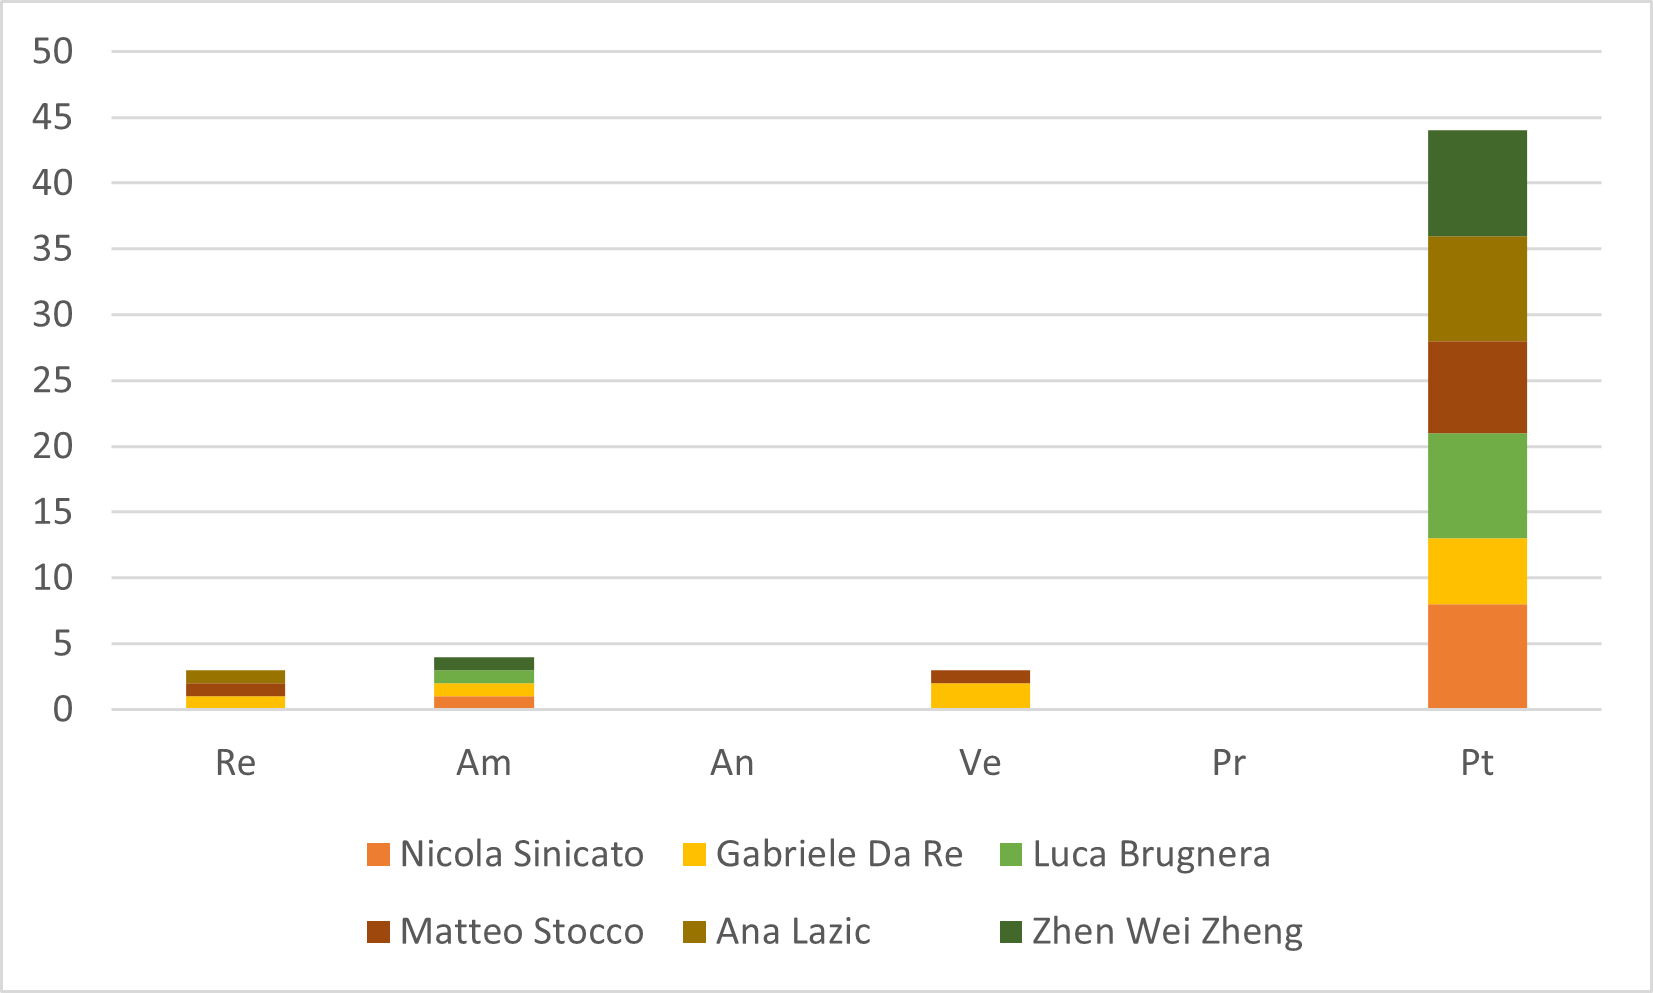
\includegraphics[scale=0.6]{img/grafi preventivo/istogrammi/architetturale/periodo2.png}
    \caption{Istogramma della ripartizione delle ore del secondo periodo della fase di progettazione architetturale}
\end{figure}
\begin{figure}[H]
    \centering
    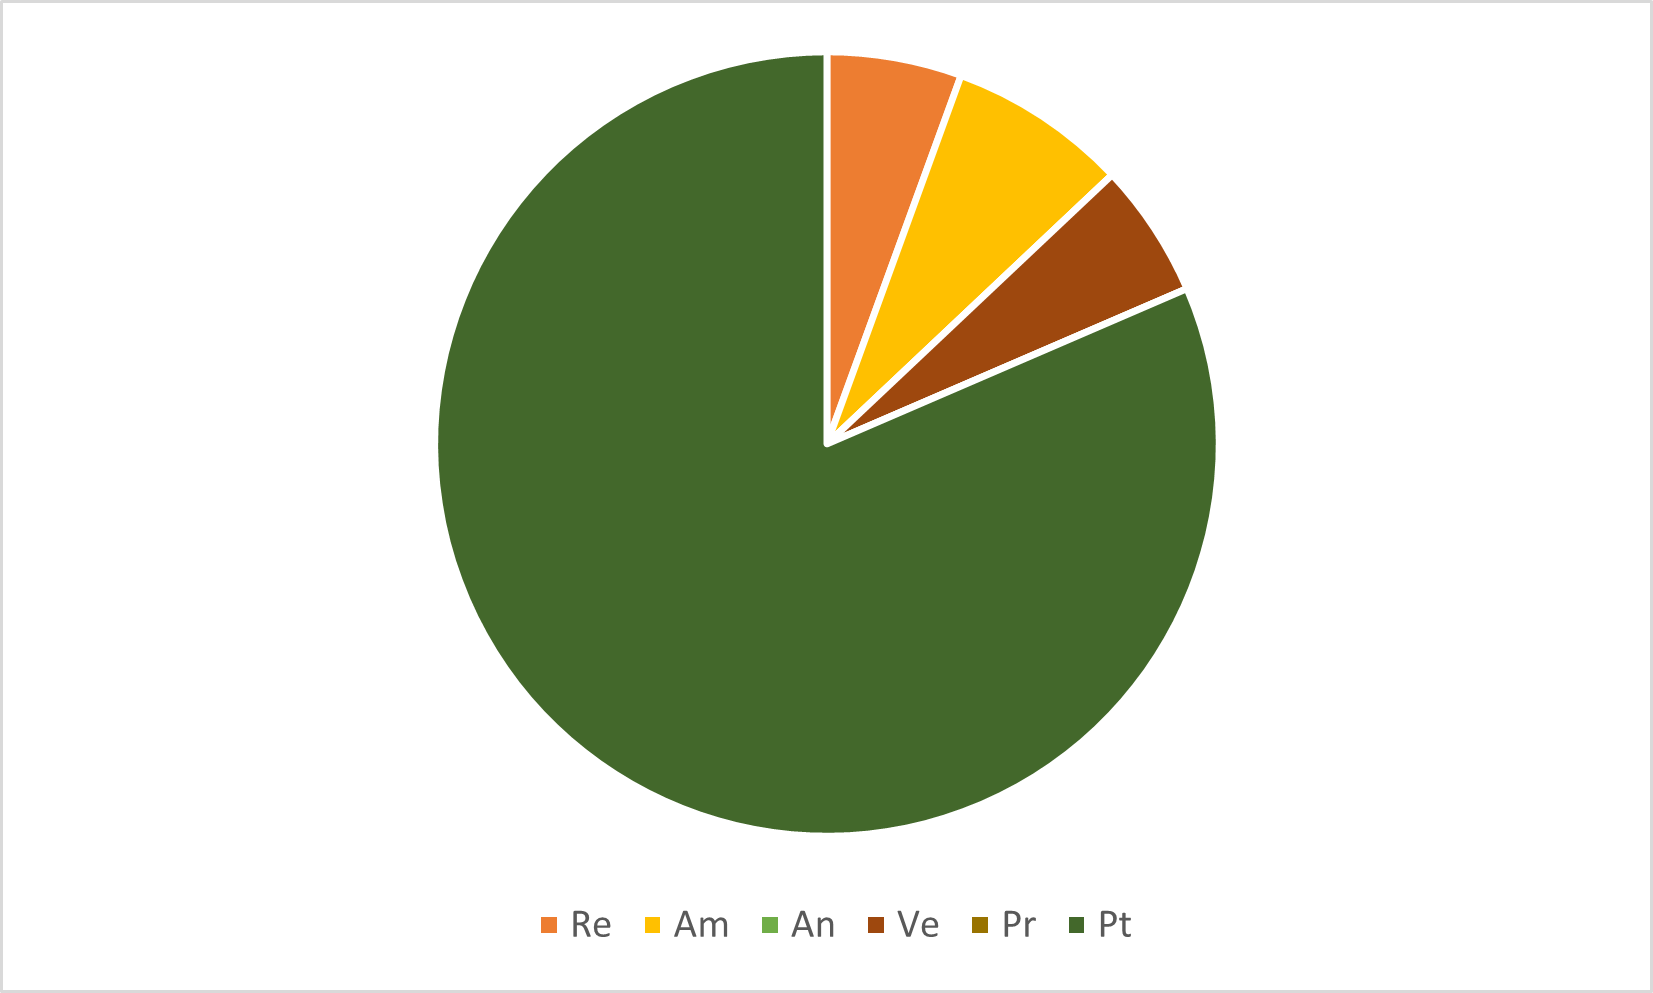
\includegraphics[scale=0.6]{img/grafi preventivo/torta/architetturale/periodo2.png}
    \caption{Grafico a torta della ripartizione delle ore per ruolo nel secondo periodo della fase di progettazione architetturale}
\end{figure}
\subsubsubsection{Preventivo dei costi}
La seguente tabella rappresenta le ore dedicate ad ogni ruolo e il corrispettivo costo in euro per il secondo periodo della fase di progettazione architetturale:

	\setlength\extrarowheight{5pt}
	\rowcolors{2}{gray!10}{gray!40}
	\begin{tabularx}{\textwidth}{|ccc|c|}
		\hline
		\rowcolor{white}
		\textbf{Ruolo} & \textbf{Costo orario (€)} & \textbf{Ore totali} & \textbf{Costo totale (€)} \\
		\hline
		Responsabile &30&3&90 \\
		Amministratore &20&4&80 \\
		Analista &25&0&0 \\
		Verificatore &15&6&90 \\
		Programmatore &15&0&0 \\
		Progettista &25&41&1025 \\
		\hline
		Totale &-&-&1285 \\
		\hline
		\rowcolor{white}
		\caption{Prospetto del costo orario durante il secondo periodo di progettazione architetturale per ruolo}
	\end{tabularx}
    \vspace{10pt}
	
% ----------------------------------------------------------------------------------------------------------------
\newpage
\subsubsection{Riepilogo della fase di progettazione architetturale }
% ----------------------------------------------------------------------------------------------------------------
%
\subsubsubsection{Preventivo orario}
La seguente tabella rappresenta la distribuzione oraria per ogni componente per la fase di progettazione architetturale:

	\setlength\extrarowheight{5pt}
	\rowcolors{2}{gray!10}{gray!40}
	\begin{tabularx}{\textwidth}{|ccccccc|c|}
		\hline
		\rowcolor{white}
		\textbf{Nome} & \textbf{Re} & \textbf{Am} & \textbf{An} & \textbf{Ve} & \textbf{Pr}& \textbf{Pt} & \textbf{Ore totali} \\
		\hline
		Nicola Sinicato &1&2&1&0&0&9&13 \\
		Gabriele Da Re &1&1&0&4&0&7&13 \\
		Luca Brugnera &1&2&1&0&0&9&13 \\
		Matteo Stocco &1&1&0&4&0&7&13 \\
		Ana Lazic &1&1&1&1&0&9&13 \\
		Zhen Wei Zheng &1&1&0&2&0&9&13 \\
		\hline
		Ore totali ruolo &6&8&3&11&0&50&78 \\
		\hline
		\rowcolor{white}
		\caption{Distribuzione oraria durante la fase di progettazione architetturale per ruolo e persona}
	\end{tabularx}
	\vspace{10pt}
	
\begin{figure}[H]
    \centering
    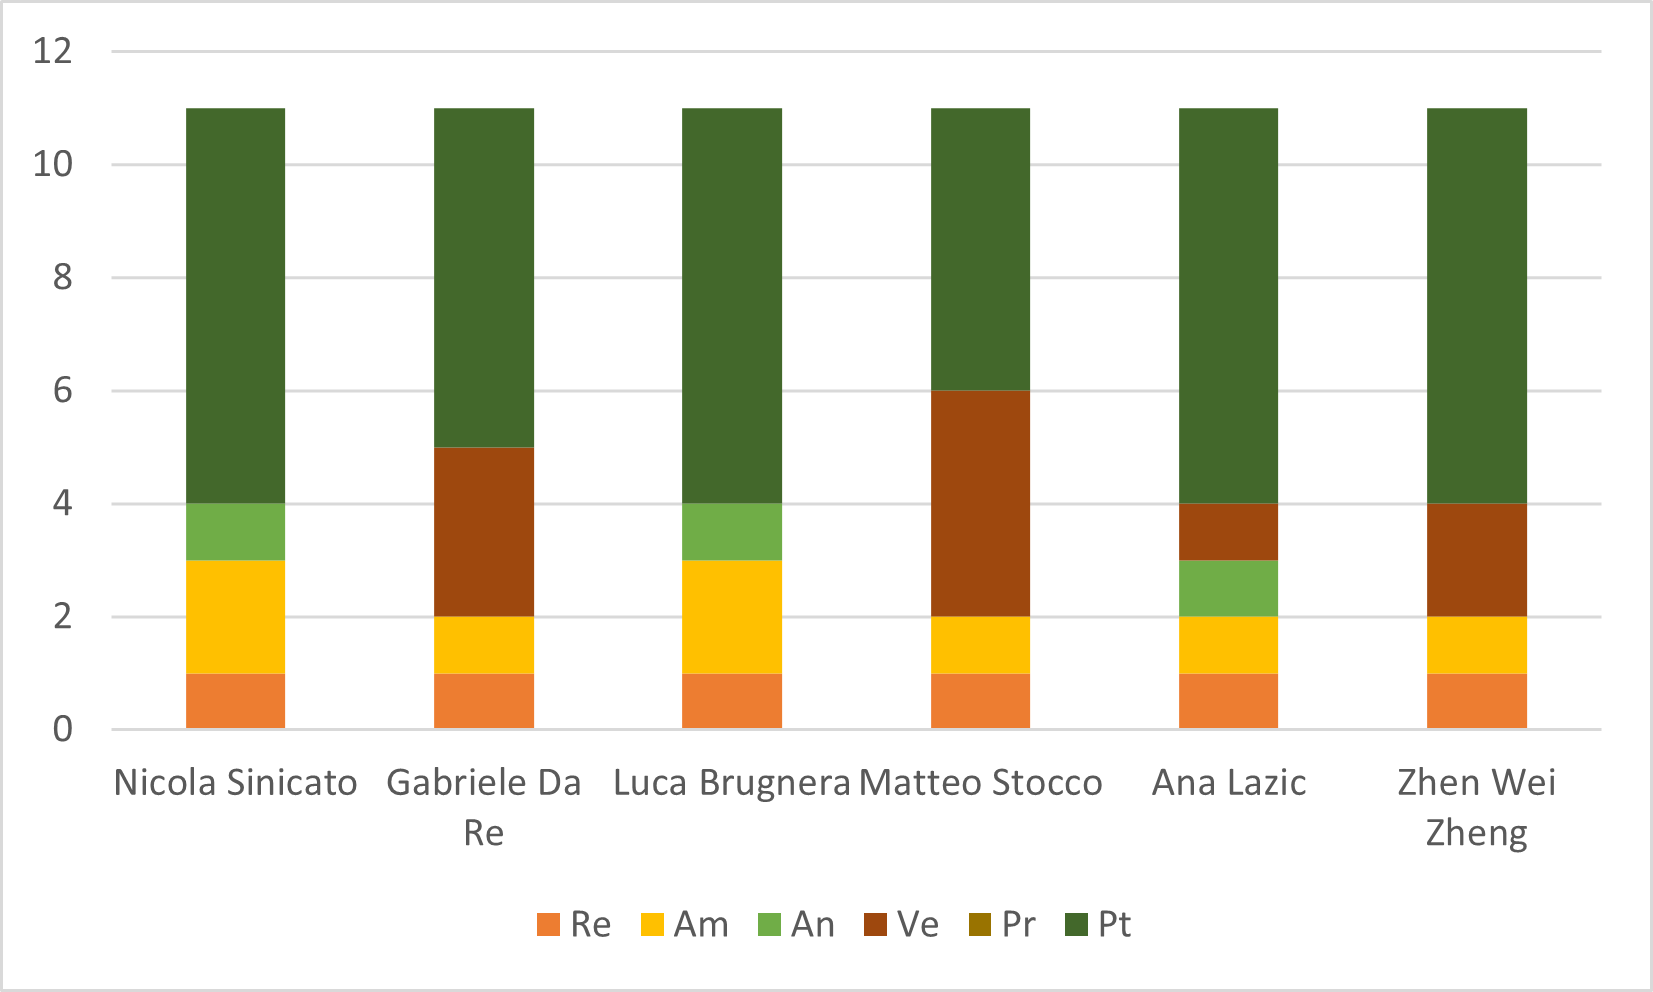
\includegraphics[scale=0.6]{img/grafi preventivo/istogrammi/architetturale/complessivo.png}
    \caption{Istogramma della ripartizione delle ore della fase di progettazione architetturale}
\end{figure}
\begin{figure}[H]
    \centering
    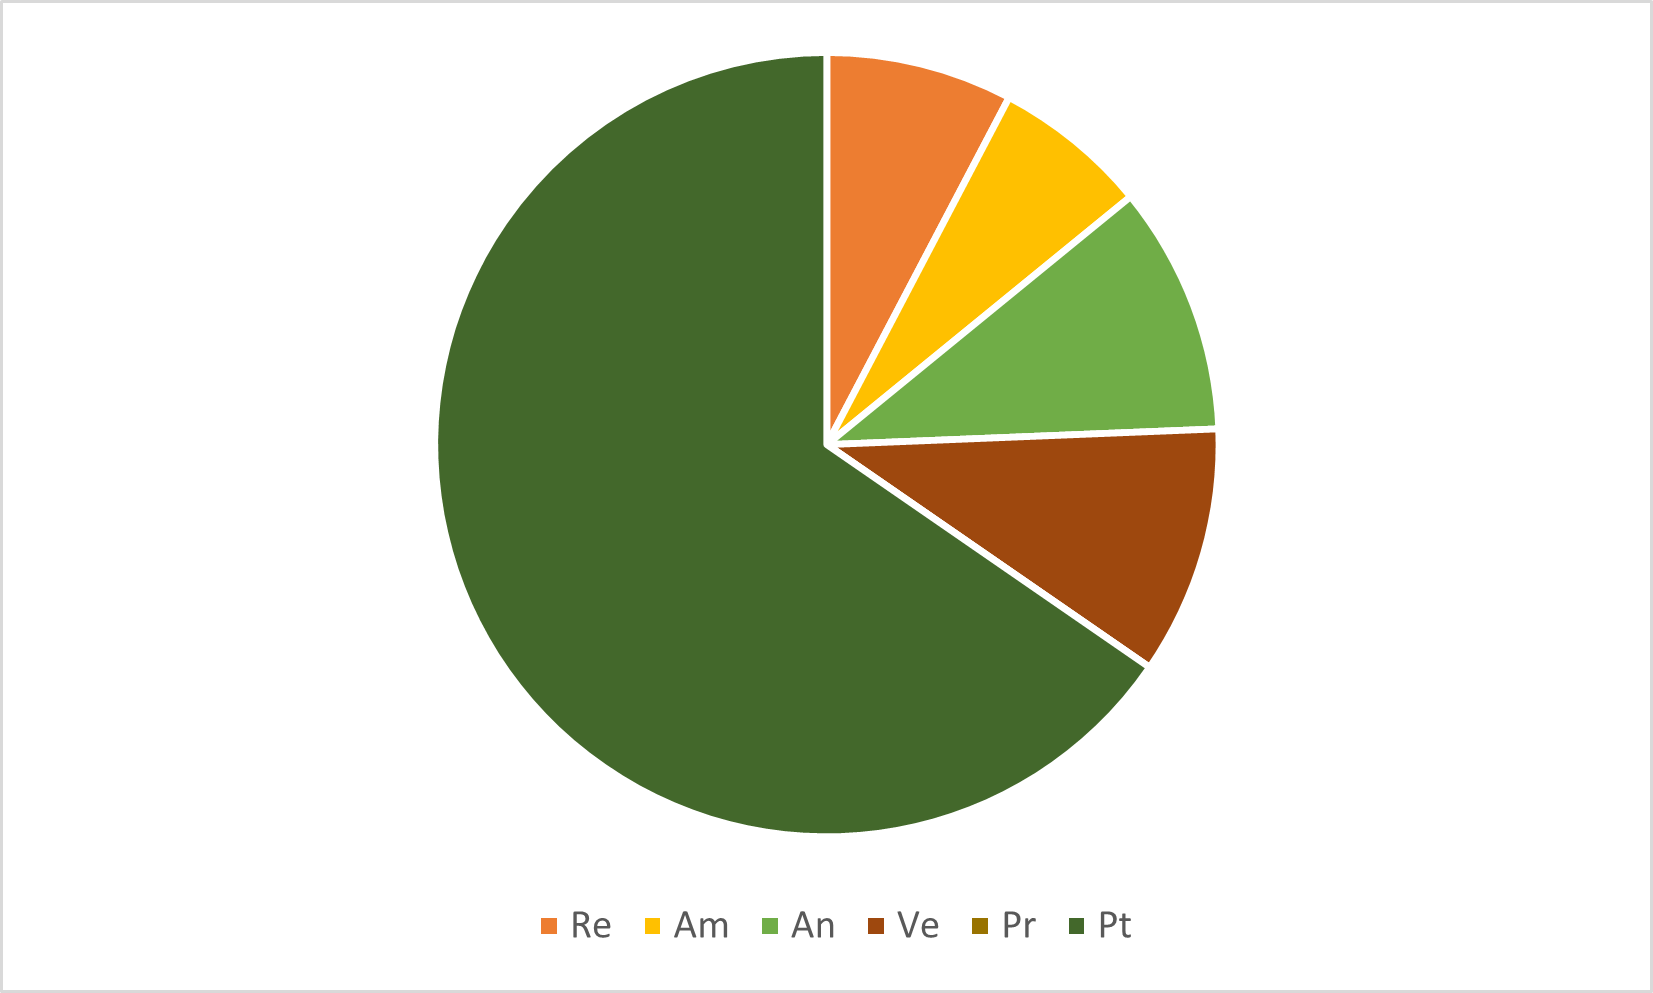
\includegraphics[scale=0.6]{img/grafi preventivo/torta/architetturale/complessivo.png}
    \caption{Grafico a torta della ripartizione delle ore per ruolo nella fase di progettazione architetturale}
\end{figure}
\subsubsubsection{Preventivo dei costi}
La seguente tabella rappresenta le ore dedicate ad ogni ruolo e il corrispettivo costo in euro per la fase di progettazione architetturale:

	\setlength\extrarowheight{5pt}
	\rowcolors{2}{gray!10}{gray!40}
	\begin{tabularx}{\textwidth}{|ccc|c|}
		\hline
		\rowcolor{white}
		\textbf{Ruolo} & \textbf{Costo orario (€)} & \textbf{Ore totali} & \textbf{Costo totale (€)} \\
		\hline
		Responsabile &30&6&180 \\
		Amministratore &20&8&160 \\
		Analista &25&3&75 \\
		Verificatore &15&11&165 \\
		Programmatore &15&0&0 \\
		Progettista &25&50&1250 \\
		\hline
		Totale &-&-&1830 \\
		\hline
		\rowcolor{white}
		\caption{Prospetto del costo orario durante la fase di progettazione architetturale per ruolo}
	\end{tabularx}
    \vspace{10pt}
	

% ----------------------------------------------------------------------------------------------------------------
\newpage
\subsection{Progettazione di dettaglio e codifica}
% ----------------------------------------------------------------------------------------------------------------
\subsubsection{Periodo 1}
% ----------------------------------------------------------------------------------------------------------------
%
\subsubsubsection{Preventivo orario}
La seguente tabella rappresenta la distribuzione oraria per ogni componente per il primo periodo di fase di progettazione di dettaglio e codifica:

	\setlength\extrarowheight{5pt}
	\rowcolors{2}{gray!10}{gray!40}
	\begin{tabularx}{\textwidth}{|ccccccc|c|}
		\hline
		\rowcolor{white}
		\textbf{Nome} & \textbf{Re} & \textbf{Am} & \textbf{An} & \textbf{Ve} & \textbf{Pr}& \textbf{Pt} & \textbf{Ore totali} \\
		\hline
		Nicola Sinicato &1&0&0&0&1&1&3 \\
		Gabriele Da Re &0&0&0&0&0&2&1 \\
		Luca Brugnera &0&1&0&2&0&0&3 \\
		Matteo Stocco &1&0&0&0&0&2&3 \\
		Ana Lazic &0&0&0&0&2&1&3 \\
		Zhen Wei Zheng &0&1&0&2&0&0&3 \\
		\hline
		Ore totali ruolo &2&2&0&4&5&5&18 \\
		\hline
		\rowcolor{white}
		\caption{Distribuzione oraria durante il primo periodo di progettazione di dettaglio e codifica per ruolo e persona}
	\end{tabularx}
	\vspace{10pt}
	
\begin{figure}[H]
    \centering
    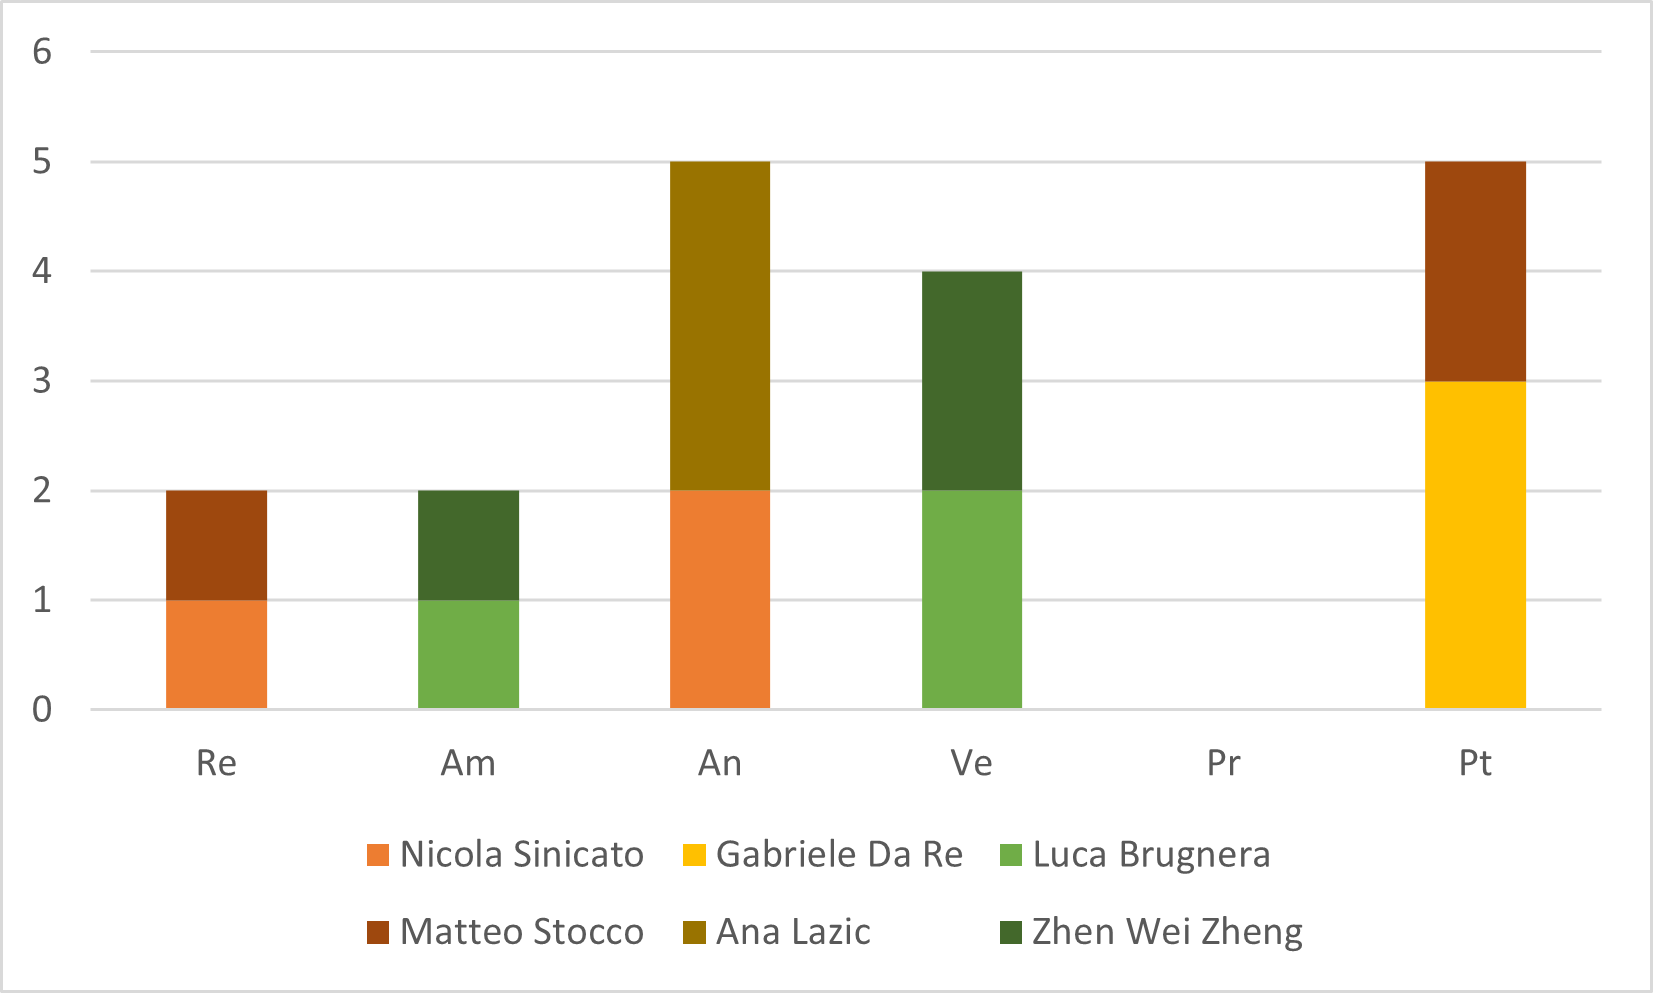
\includegraphics[scale=0.6]{img/grafi preventivo/istogrammi/codifica/periodo1.png}
    \caption{Istogramma della ripartizione delle ore del primo periodo della fase di progettazione di dettaglio e codifica}
\end{figure}
\begin{figure}[H]
    \centering
    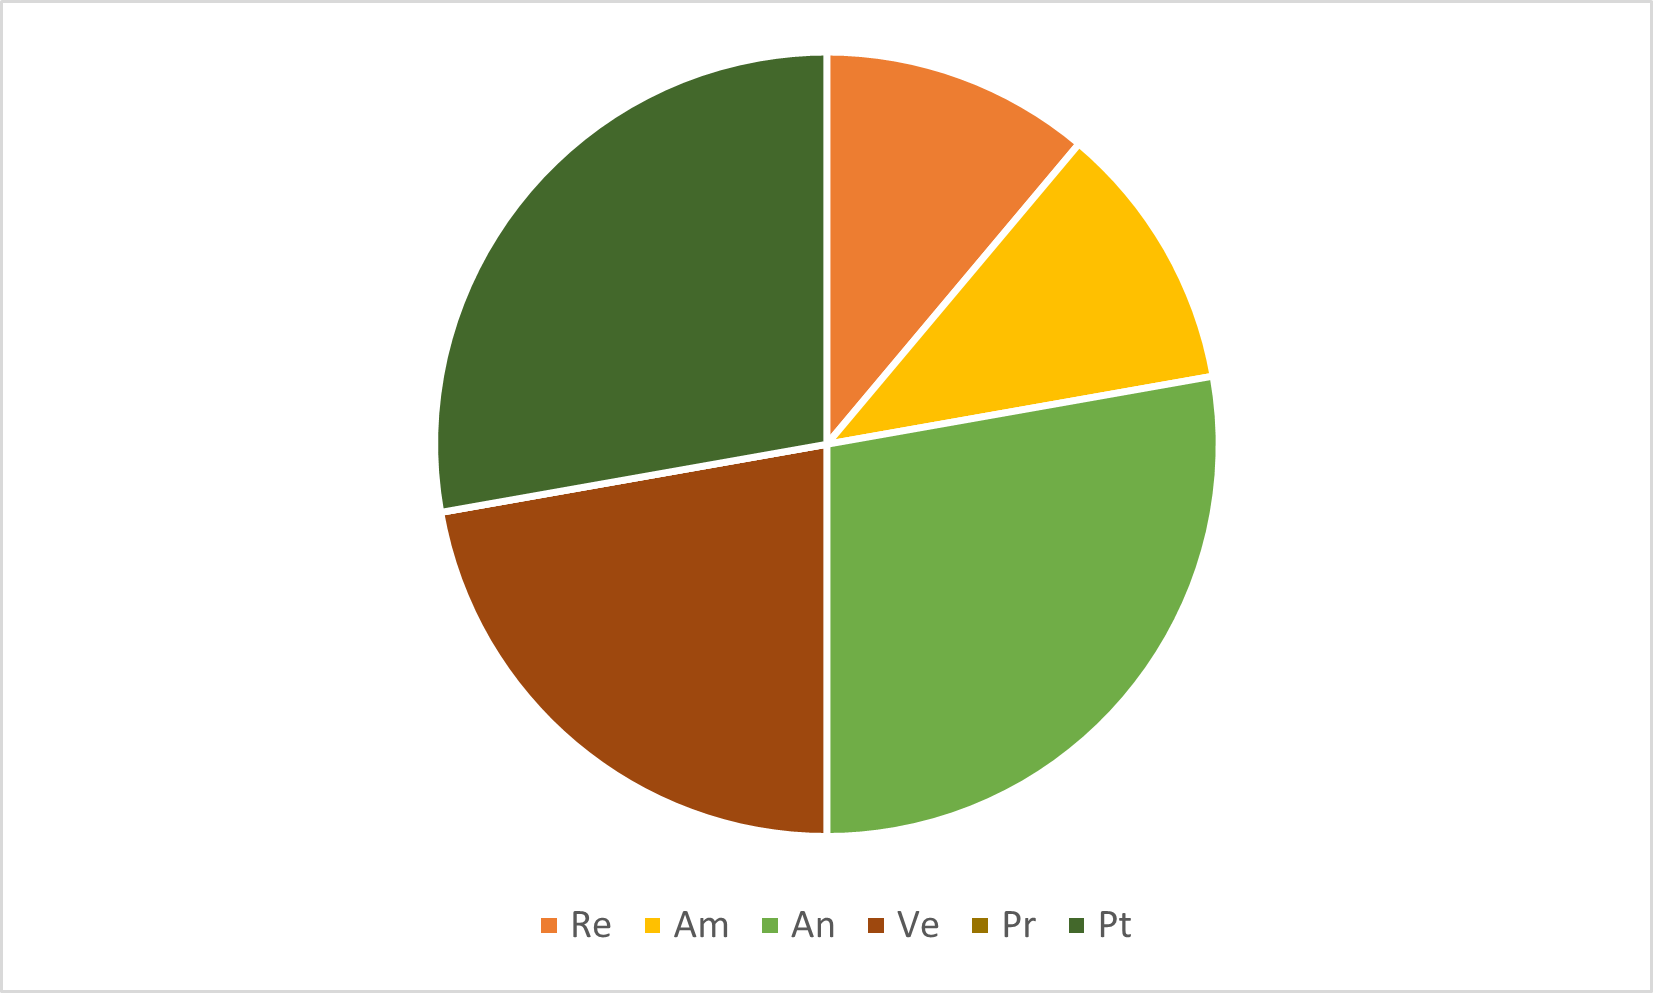
\includegraphics[scale=0.6]{img/grafi preventivo/torta/codifica/periodo1.png}
    \caption{Grafico a torta della ripartizione delle ore per ruolo nel primo periodo della fase di progettazione di dettaglio e codifica}
\end{figure}
\subsubsubsection{Preventivo dei costi}
La seguente tabella rappresenta le ore dedicate ad ogni ruolo e il corrispettivo costo in euro per il primo periodo della fase di progettazione di dettaglio e codifica:

	\setlength\extrarowheight{5pt}
	\rowcolors{2}{gray!10}{gray!40}
	\begin{tabularx}{\textwidth}{|ccc|c|}
		\hline
		\rowcolor{white}
		\textbf{Ruolo} & \textbf{Costo orario (€)} & \textbf{Ore totali} & \textbf{Costo totale (€)} \\
		\hline
		Responsabile &30&2&60 \\
		Amministratore &20&2&40 \\
		Analista &25&0&0 \\
		Verificatore &15&4&60 \\
		Programmatore &15&5&75 \\
		Progettista &25&5&125 \\
		\hline
		Totale &-&-&360 \\
		\hline
		\rowcolor{white}
		\caption{Prospetto del costo orario durante il primo periodo di progettazione di dettaglio e codifica per ruolo}
	\end{tabularx}
    \vspace{10pt}
	
%
% ----------------------------------------------------------------------------------------------------------------
\newpage
\subsubsection{Periodo 2}
% ----------------------------------------------------------------------------------------------------------------
%
\subsubsubsection{Preventivo orario}
La seguente tabella rappresenta la distribuzione oraria per ogni componente per il secondo periodo della fase di progettazione di dettaglio e codifica:

	\setlength\extrarowheight{5pt}
	\rowcolors{2}{gray!10}{gray!40}
	\begin{tabularx}{\textwidth}{|ccccccc|c|}
		\hline
		\rowcolor{white}
		\textbf{Nome} & \textbf{Re} & \textbf{Am} & \textbf{An} & \textbf{Ve} & \textbf{Pr}& \textbf{Pt} & \textbf{Ore totali} \\
		\hline
		Nicola Sinicato &0&0&0&2&14&0&16 \\
		Gabriele Da Re &0&1&0&1&11&3&16 \\
		Luca Brugnera &0&1&0&1&11&3&16 \\
		Matteo Stocco &0&0&0&2&14&0&16 \\
		Ana Lazic &1&0&0&2&11&2&16 \\
		Zhen Wei Zheng &1&2&0&2&11&0&16 \\
		\hline
		Ore totali ruolo &2&4&0&10&72&8&96 \\
		\hline
		\rowcolor{white}
		\caption{Distribuzione oraria durante  il secondo periodo di progettazione di dettaglio e codifica per ruolo e persona}
	\end{tabularx}
	\vspace{10pt}
	
\begin{figure}[H]
    \centering
    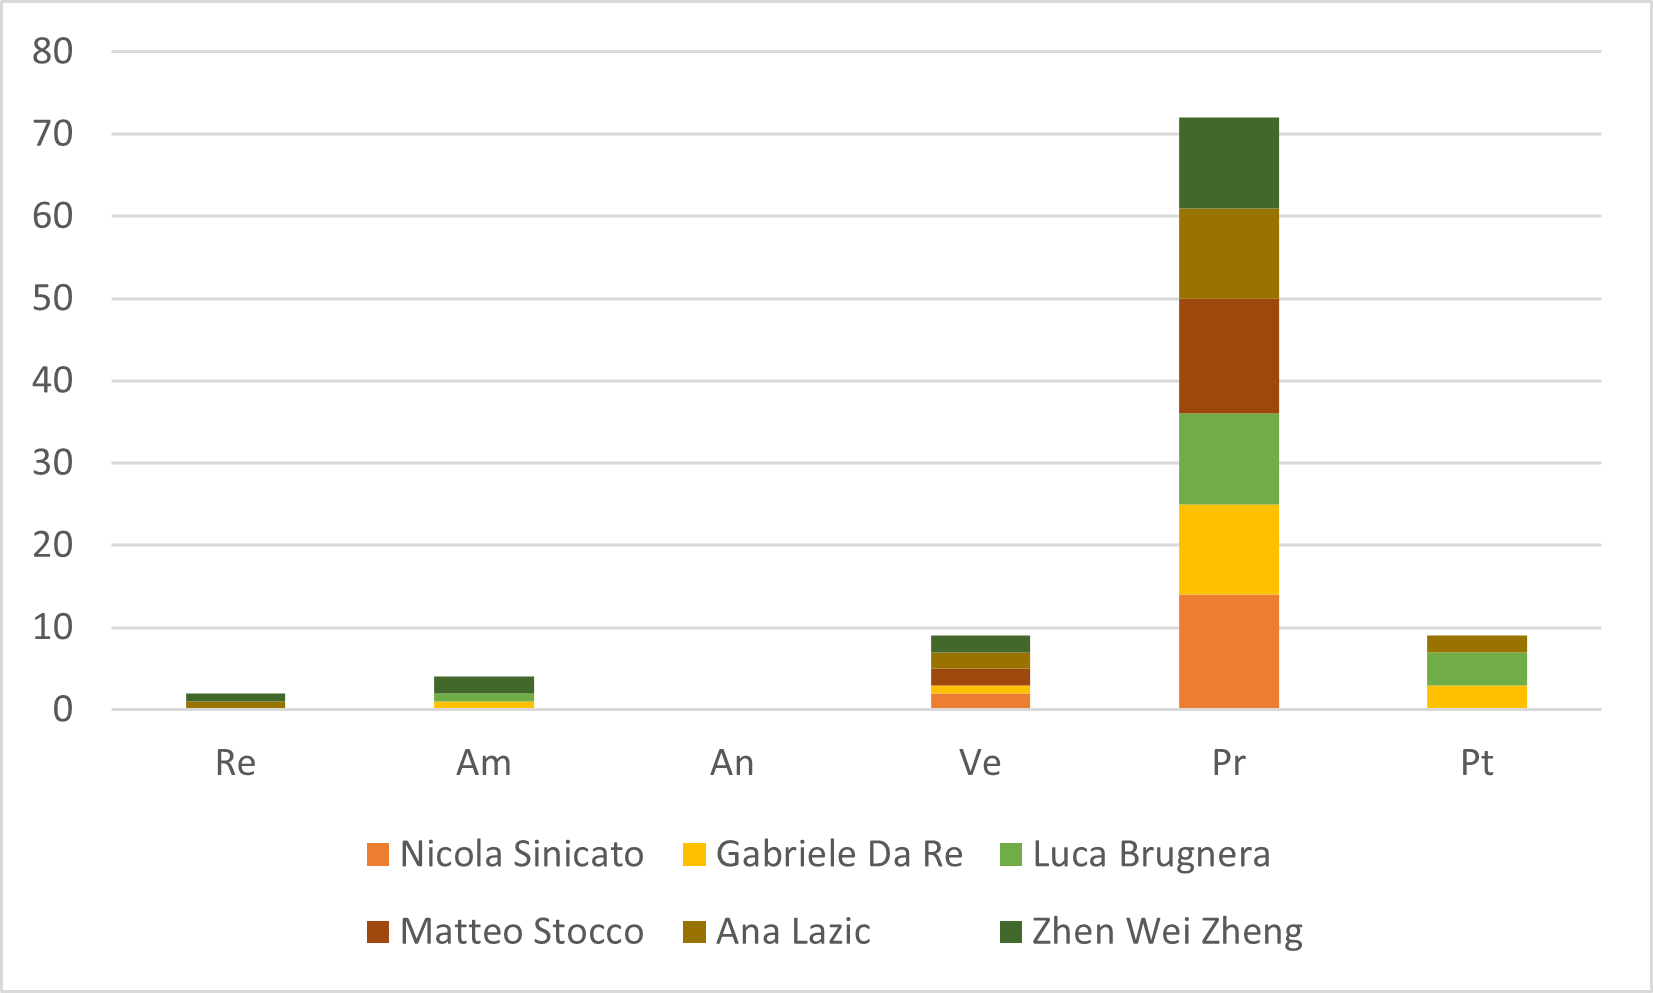
\includegraphics[scale=0.6]{img/grafi preventivo/istogrammi/codifica/periodo2.png}
    \caption{Istogramma della ripartizione delle ore del secondo periodo della fase di progettazione di dettaglio e codifica}
\end{figure}
\begin{figure}[H]
    \centering
    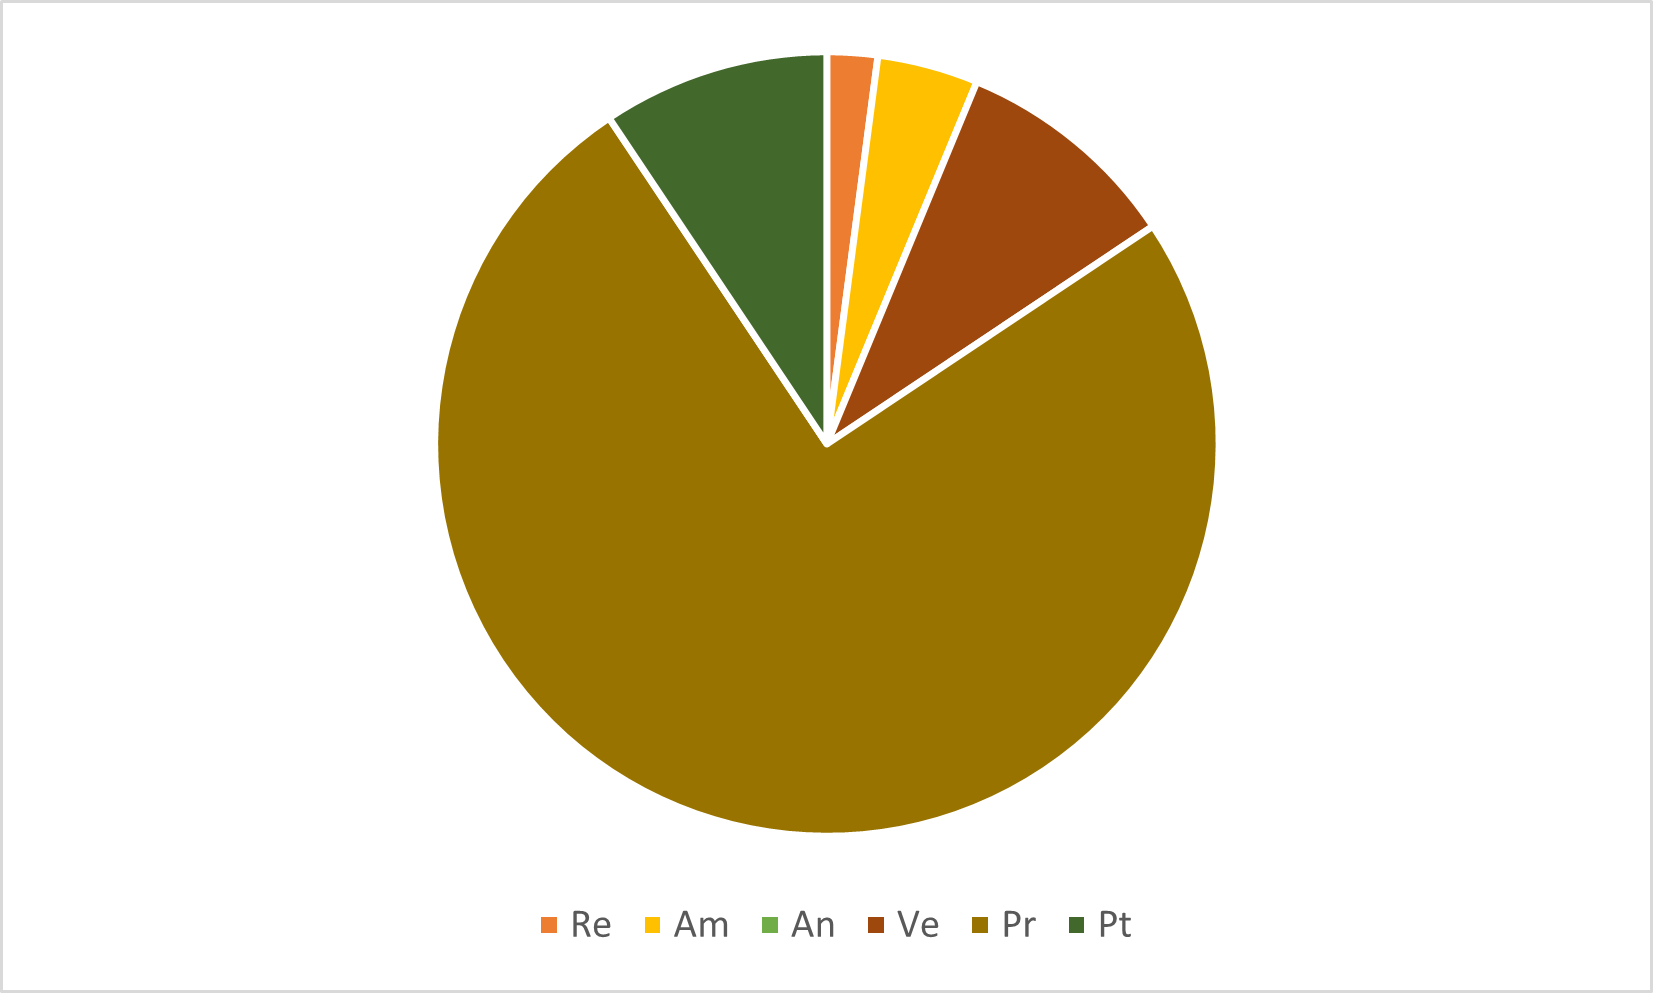
\includegraphics[scale=0.6]{img/grafi preventivo/torta/codifica/periodo2.png}
    \caption{Grafico a torta della ripartizione delle ore per ruolo nel secondo periodo della fase di progettazione di dettaglio e codifica}
\end{figure}
\subsubsubsection{Preventivo dei costi}
La seguente tabella rappresenta le ore dedicate ad ogni ruolo e il corrispettivo costo in euro per il secondo periodo della fase di progettazione di dettaglio e codifica:

	\setlength\extrarowheight{5pt}
	\rowcolors{2}{gray!10}{gray!40}
	\begin{tabularx}{\textwidth}{|ccc|c|}
		\hline
		\rowcolor{white}
		\textbf{Ruolo} & \textbf{Costo orario (€)} & \textbf{Ore totali} & \textbf{Costo totale (€)} \\
		\hline
		Responsabile &30&2&60 \\
		Amministratore &20&4&80 \\
		Analista &25&0&0 \\
		Verificatore &15&10&150 \\
		Programmatore &15&72&1080 \\
		Progettista &25&8&200 \\
		\hline
		Totale &-&-&1570 \\
		\hline
		\rowcolor{white}
		\caption{Prospetto del costo orario durante  il secondo periodo di progettazione di dettaglio e codifica per ruolo}
	\end{tabularx}
    \vspace{10pt}
	
%
% ----------------------------------------------------------------------------------------------------------------
\newpage
\subsubsection{Periodo 3}
% ----------------------------------------------------------------------------------------------------------------
%
\subsubsubsection{Preventivo orario}
La seguente tabella rappresenta la distribuzione oraria per ogni componente per il terzo periodo della fase di progettazione di dettaglio e codifica:

	\setlength\extrarowheight{5pt}
	\rowcolors{2}{gray!10}{gray!40}
	\begin{tabularx}{\textwidth}{|ccccccc|c|}
		\hline
		\rowcolor{white}
		\textbf{Nome} & \textbf{Re} & \textbf{Am} & \textbf{An} & \textbf{Ve} & \textbf{Pr}& \textbf{Pt} & \textbf{Ore totali} \\
		\hline
		Nicola Sinicato &0&0&0&2&1&0&3 \\
		Gabriele Da Re &1&2&0&0&0&0&3 \\
		Luca Brugnera &0&0&0&1&2&0&3 \\
		Matteo Stocco &0&0&0&2&1&0&3 \\
		Ana Lazic &1&2&0&0&0&0&3 \\
		Zhen Wei Zheng &1&0&0&2&0&0&3 \\
		\hline
		Ore totali ruolo &3&4&0&7&4&0&18 \\
		\hline
		\rowcolor{white}
		\caption{Distribuzione oraria durante  il terzo periodo di progettazione di dettaglio e codifica per ruolo e persona}
	\end{tabularx}
	\vspace{10pt}
	
\begin{figure}[H]
    \centering
    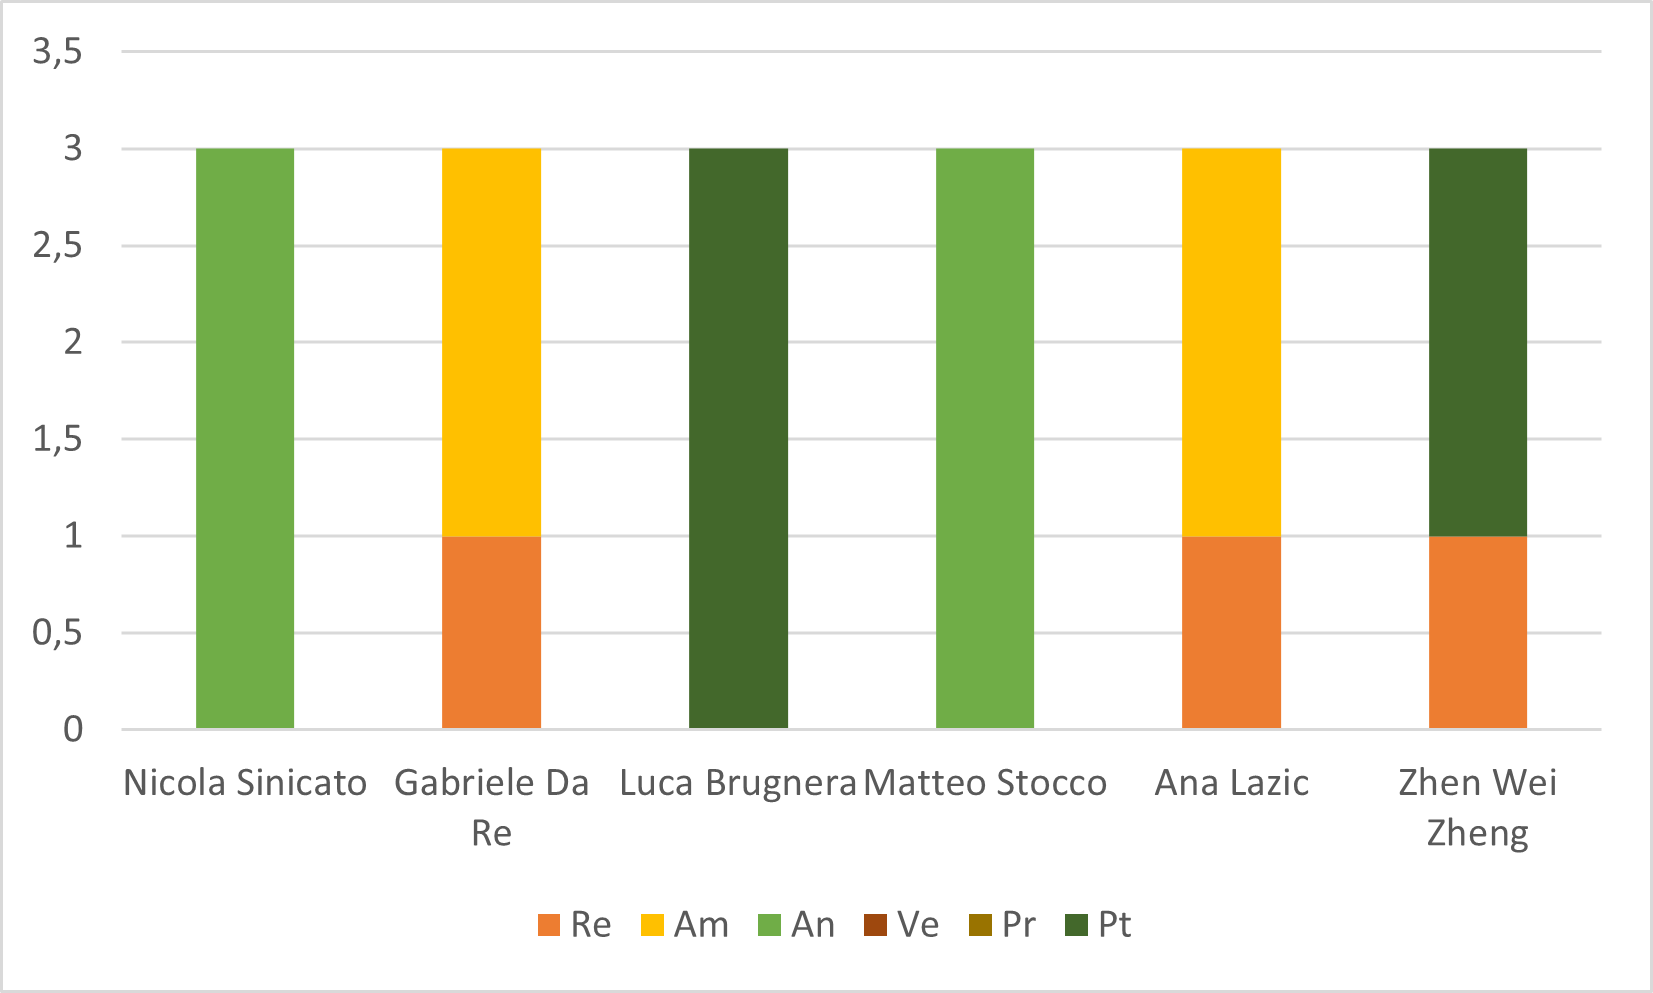
\includegraphics[scale=0.6]{img/grafi preventivo/istogrammi/codifica/periodo3.png}
    \caption{Istogramma della ripartizione delle ore del terzo periodo della fase di progettazione di dettaglio e codifica}
\end{figure}
\begin{figure}[H]
    \centering
    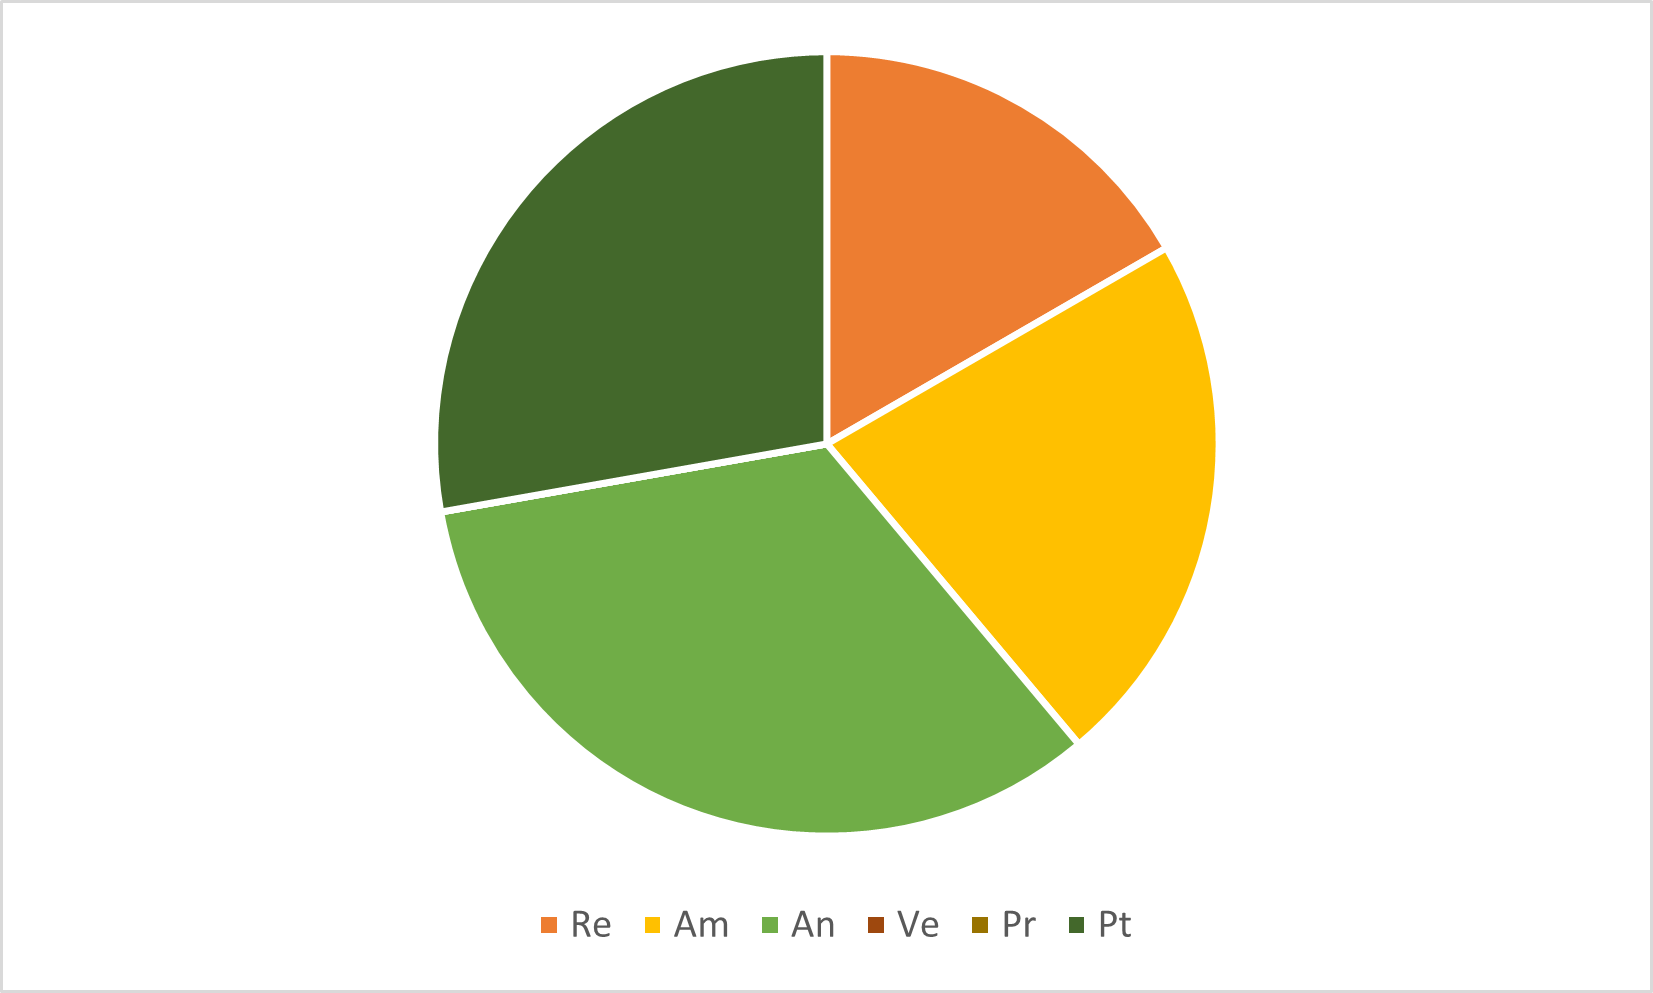
\includegraphics[scale=0.6]{img/grafi preventivo/torta/codifica/periodo3.png}
    \caption{Grafico a torta della ripartizione delle ore per ruolo nel terzo periodo della fase di progettazione di dettaglio e codifica}
\end{figure}
\subsubsubsection{Preventivo dei costi}
La seguente tabella rappresenta le ore dedicate ad ogni ruolo e il corrispettivo costo in euro per il terzo periodo della fase di progettazione di dettaglio e codifica:

	\setlength\extrarowheight{5pt}
	\rowcolors{2}{gray!10}{gray!40}
	\begin{tabularx}{\textwidth}{|ccc|c|}
		\hline
		\rowcolor{white}
		\textbf{Ruolo} & \textbf{Costo orario (€)} & \textbf{Ore totali} & \textbf{Costo totale (€)} \\
		\hline
		Responsabile &30&3&90 \\
		Amministratore &20&4&80 \\
		Analista &25&0&0 \\
		Verificatore &15&7&105 \\
		Programmatore &15&4&60 \\
		Progettista &25&0&0 \\
		\hline
		Totale &-&-&335 \\
		\hline
		\rowcolor{white}
		\caption{Prospetto del costo orario durante  il terzo periodo di progettazione di dettaglio e codifica per ruolo}
	\end{tabularx}
    \vspace{10pt}
	
%
% ----------------------------------------------------------------------------------------------------------------
\newpage
\subsubsection{Riepilogo della fase di progettazione di dettaglio e codifica}
% ----------------------------------------------------------------------------------------------------------------
%
\subsubsubsection{Preventivo orario}
La seguente tabella rappresenta la distribuzione oraria per ogni componente la fase di progettazione di dettaglio e codifica:

	\setlength\extrarowheight{5pt}
	\rowcolors{2}{gray!10}{gray!40}
	\begin{tabularx}{\textwidth}{|ccccccc|c|}
		\hline
		\rowcolor{white}
		\textbf{Nome} & \textbf{Re} & \textbf{Am} & \textbf{An} & \textbf{Ve} & \textbf{Pr}& \textbf{Pt} & \textbf{Ore totali} \\
		\hline
		Nicola Sinicato &1&0&0&4&16&1&22 \\
		Gabriele Da Re &1&3&0&1&13&4&22 \\
		Luca Brugnera &0&2&0&4&13&3&22 \\
		Matteo Stocco &1&0&0&4&15&2&22 \\
		Ana Lazic &2&2&0&2&13&3&22 \\
		Zhen Wei Zheng &2&3&0&6&11&0&22 \\
		\hline
		Ore totali ruolo &7&10&0&21&81&13&132 \\
		\hline
		\rowcolor{white}
		\caption{Distribuzione oraria durante la fase di progettazione di dettaglio e codifica per ruolo e persona}
	\end{tabularx}
	\vspace{10pt}
	
\begin{figure}[H]
    \centering
    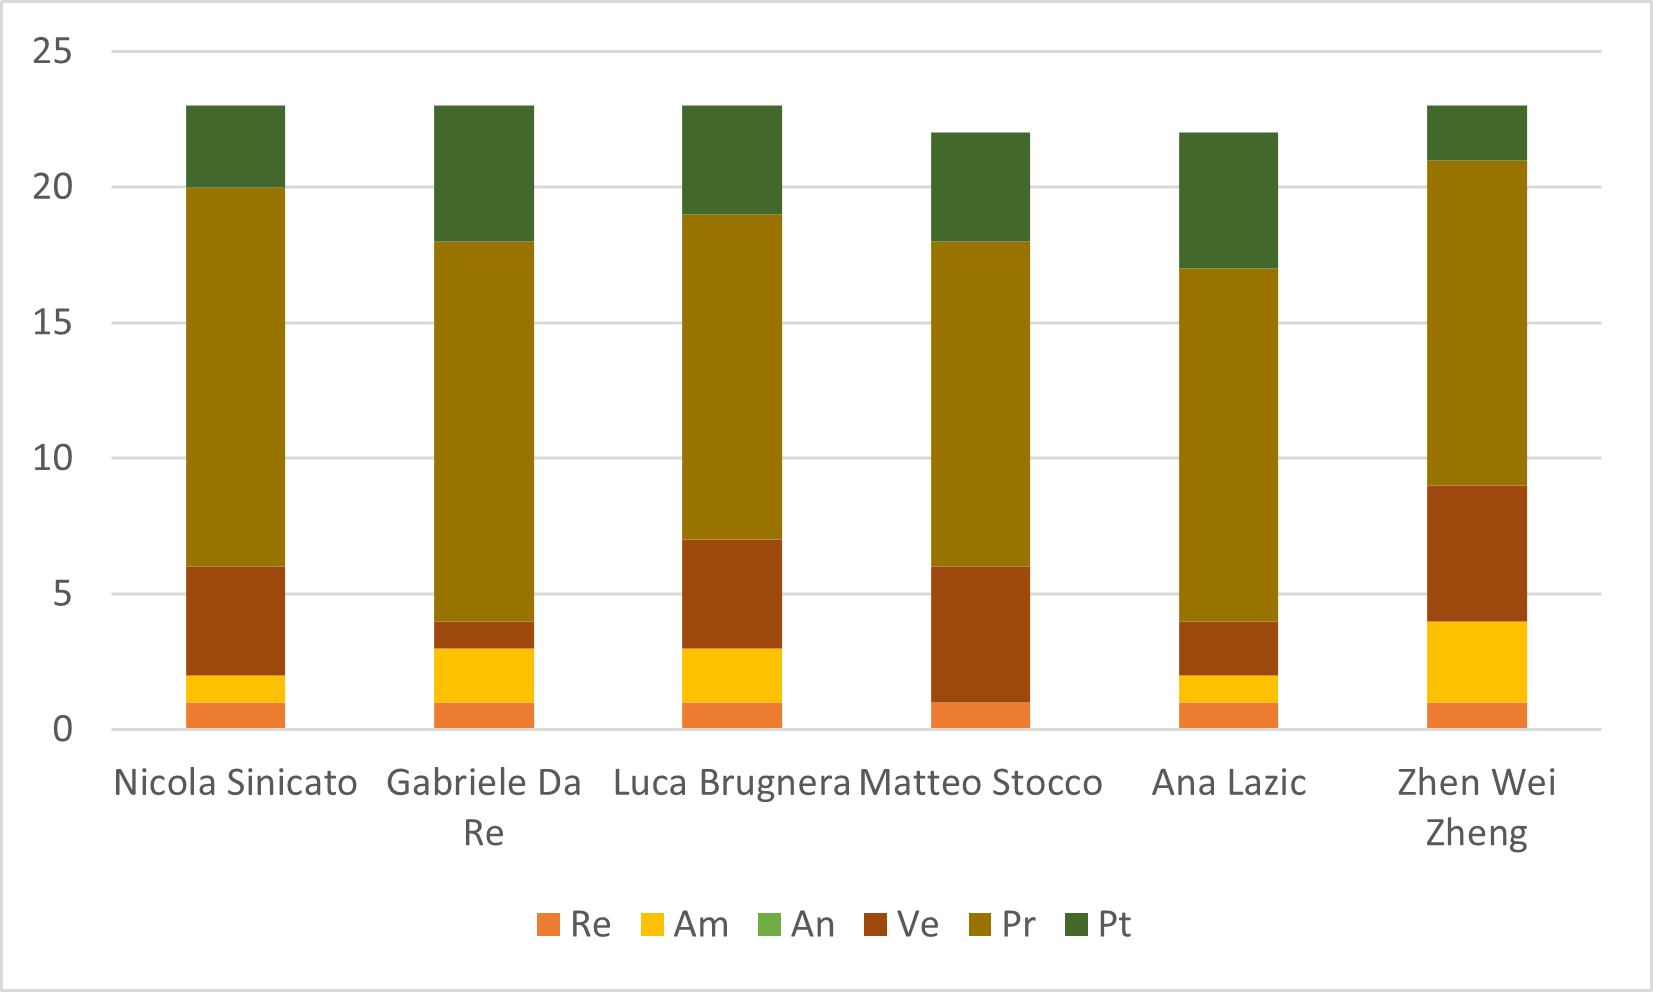
\includegraphics[scale=0.6]{img/grafi preventivo/istogrammi/codifica/complessivo.png}
    \caption{Istogramma della ripartizione delle ore della fase di progettazione di dettaglio e codifica}
\end{figure}
\begin{figure}[H]
    \centering
    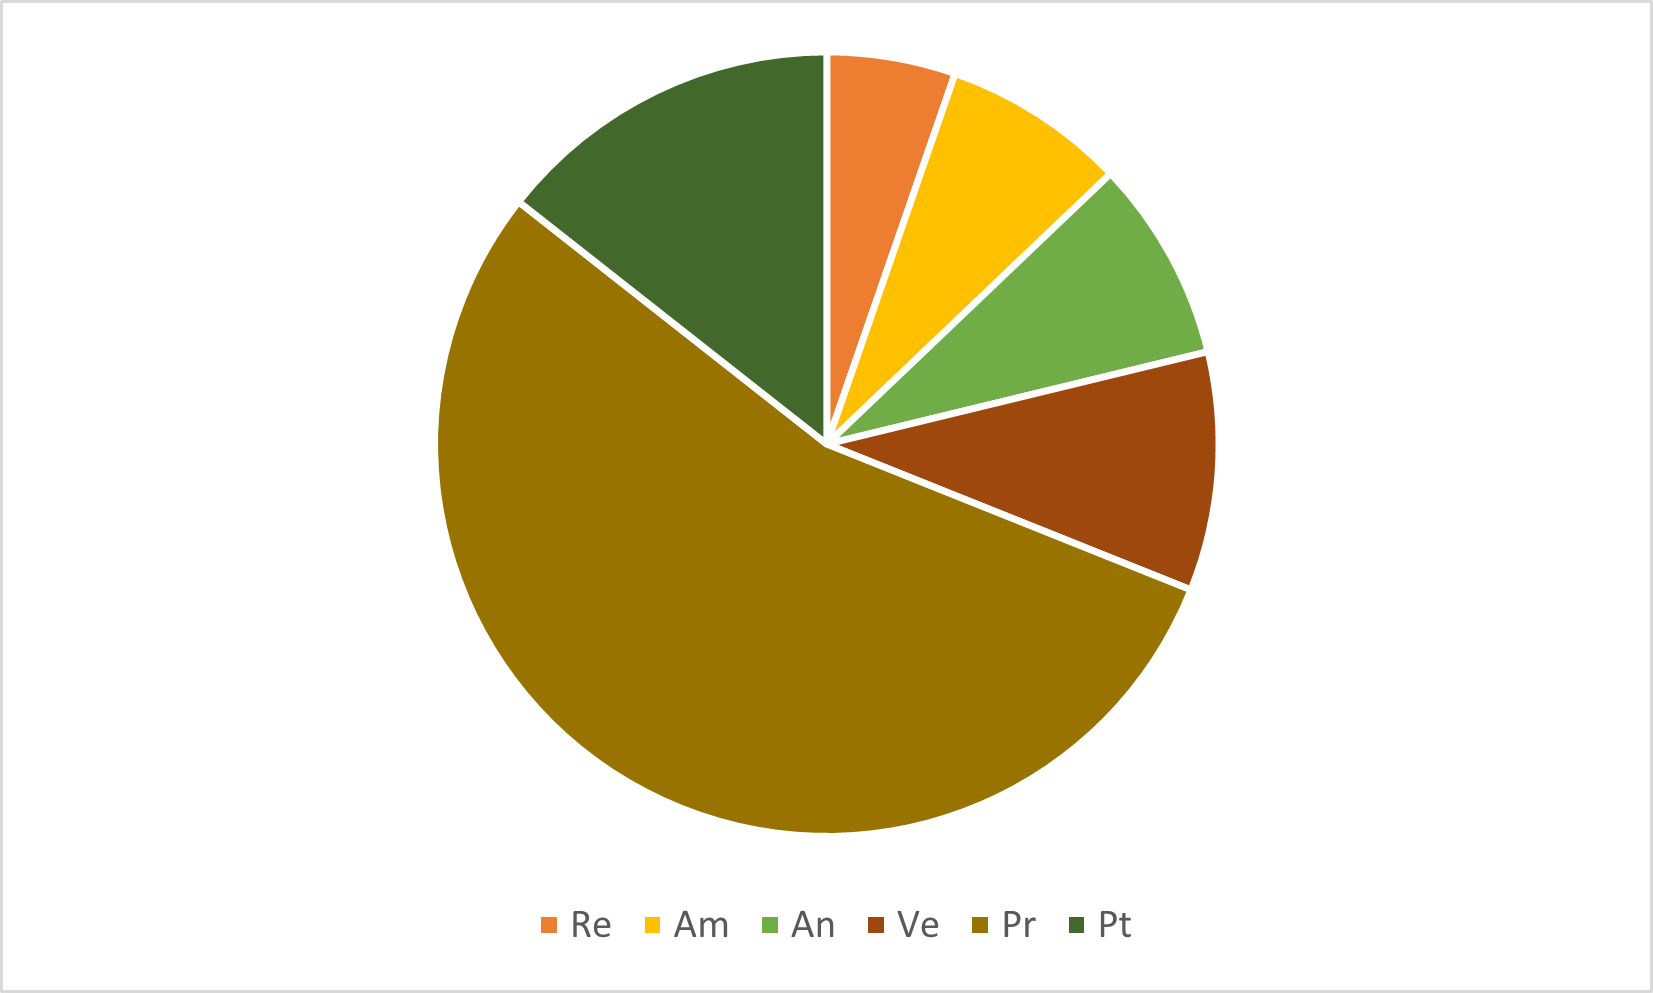
\includegraphics[scale=0.6]{img/grafi preventivo/torta/codifica/complessivo.png}
    \caption{Grafico a torta della ripartizione delle ore per ruolo nella fase di progettazione di dettaglio e codifica}
\end{figure}
\subsubsubsection{Preventivo dei costi}
La seguente tabella rappresenta le ore dedicate ad ogni ruolo e il corrispettivo costo in euro per la fase di progettazione di dettaglio e codifica:

	\setlength\extrarowheight{5pt}
	\rowcolors{2}{gray!10}{gray!40}
	\begin{tabularx}{\textwidth}{|ccc|c|}
		\hline
		\rowcolor{white}
		\textbf{Ruolo} & \textbf{Costo orario (€)} & \textbf{Ore totali} & \textbf{Costo totale (€)} \\
		\hline
		Responsabile &30&7&210 \\
		Amministratore &20&10&200 \\
		Analista &25&0&0 \\
		Verificatore &15&21&315 \\
		Programmatore &15&81&1215 \\
		Progettista &25&13&325 \\
		\hline
		Totale &-&-&2265 \\
		\hline
		\rowcolor{white}
		\caption{Prospetto del costo orario durante la fase di progettazione di dettaglio e codifica per ruolo}
	\end{tabularx}
    \vspace{10pt}
	
% ----------------------------------------------------------------------------------------------------------------
\newpage
\subsection{validazione\textsubscript{G} e collaudo}

% ----------------------------------------------------------------------------------------------------------------
\subsubsection{Periodo 1}
% ----------------------------------------------------------------------------------------------------------------
%
\subsubsubsection{Preventivo orario}
La seguente tabella rappresenta la distribuzione oraria per ogni componente per il primo periodo della fase di validazione\textsubscript{G} e collaudo:

	\setlength\extrarowheight{5pt}
	\rowcolors{2}{gray!10}{gray!40}
	\begin{tabularx}{\textwidth}{|ccccccc|c|}
		\hline
		\rowcolor{white}
		\textbf{Nome} & \textbf{Re} & \textbf{Am} & \textbf{An} & \textbf{Ve} & \textbf{Pr}& \textbf{Pt} & \textbf{Ore totali} \\
		\hline
		Nicola Sinicato &2&0&0&6&3&0&11 \\
		Gabriele Da Re &2&1&0&5&3&0&11 \\
		Luca Brugnera &1&2&0&5&3&0&11 \\
		Matteo Stocco &1&2&0&5&3&0&11 \\
		Ana Lazic &2&0&0&7&2&0&11 \\
		Zhen Wei Zheng &2&2&0&5&2&0&11 \\
		\hline
		Ore totali ruolo &10&7&0&33&16&0&66 \\
		\hline
		\rowcolor{white}
		\caption{Distribuzione oraria durante  il primo periodo di validazione\textsubscript{G} e collaudo per ruolo e persona}
	\end{tabularx}
	\vspace{10pt}
	
\begin{figure}[H]
    \centering
    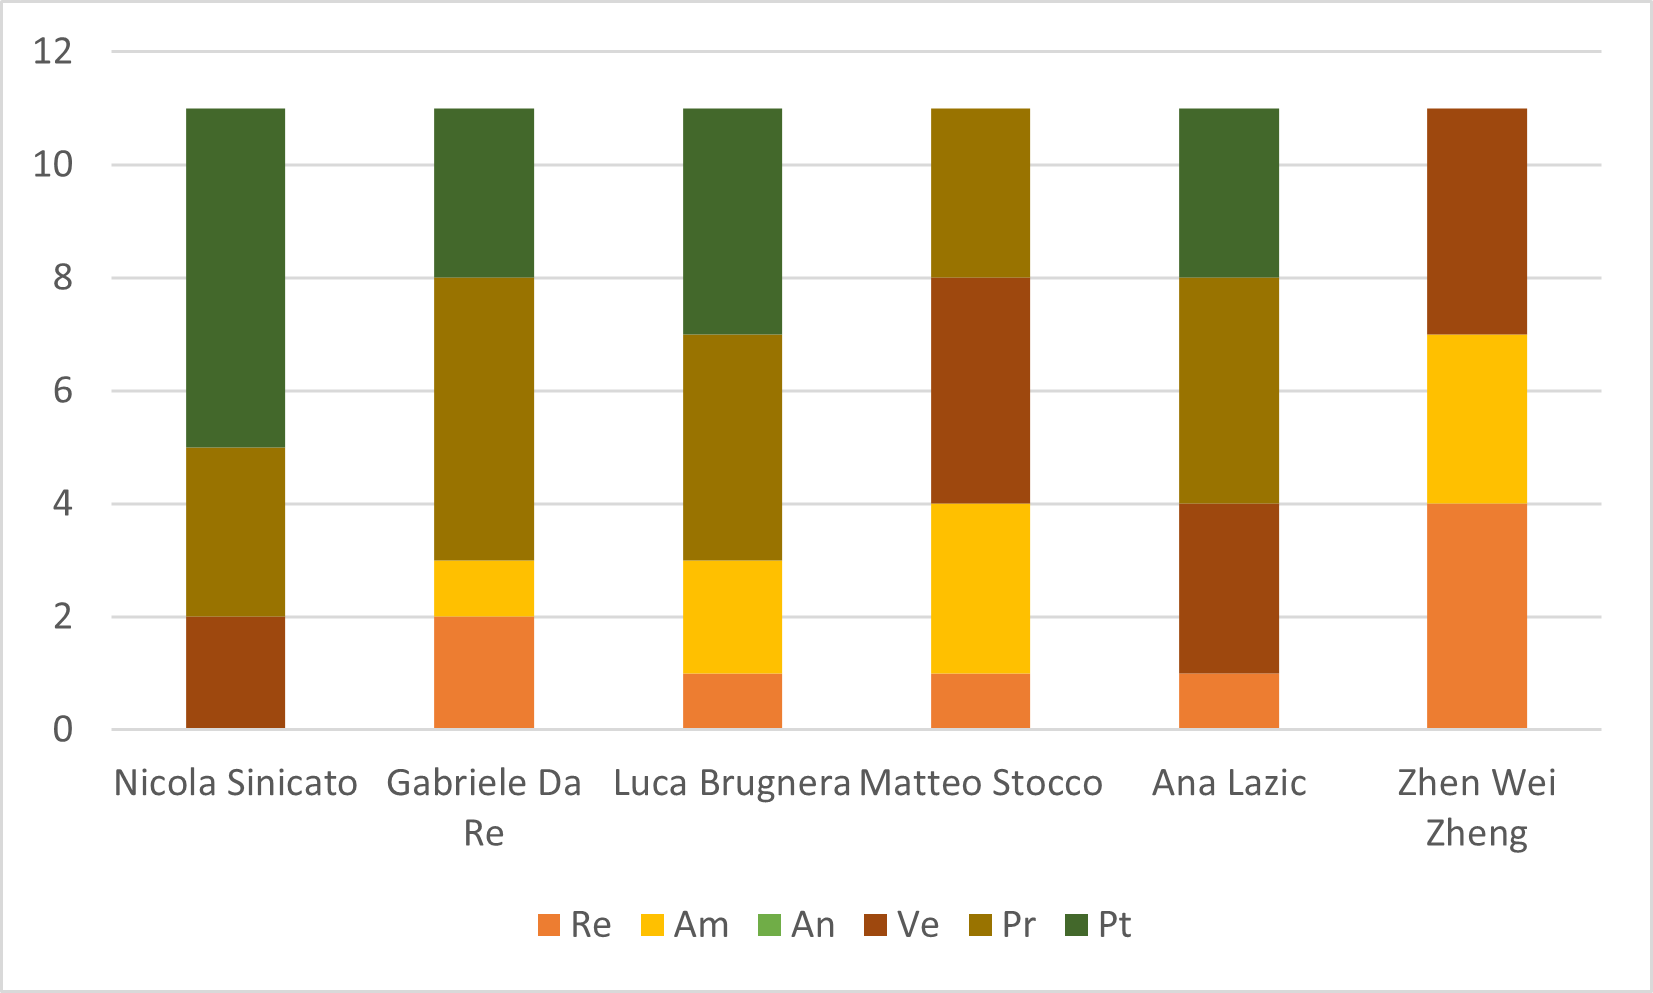
\includegraphics[scale=0.6]{img/grafi preventivo/istogrammi/validazione/periodo1.png}
    \caption{Istogramma della ripartizione delle ore del primo periodo della fase di validazione\textsubscript{G} e collaudo}
\end{figure}
\begin{figure}[H]
    \centering
    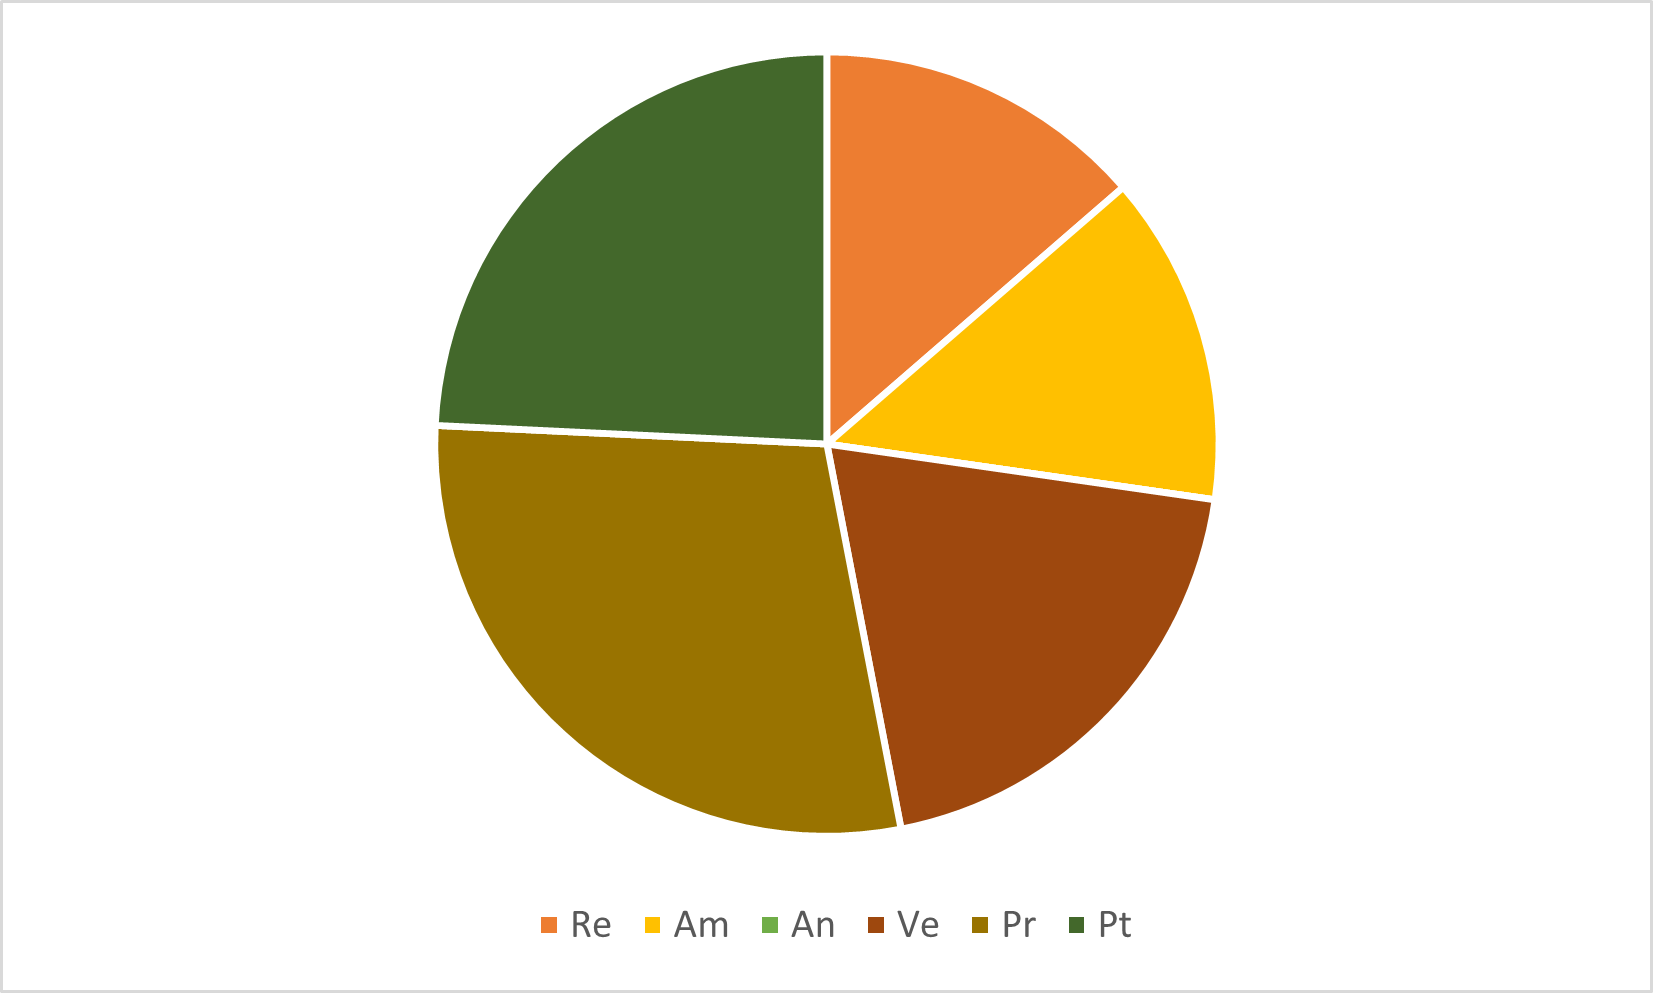
\includegraphics[scale=0.6]{img/grafi preventivo/torta/validazione/periodo1.png}
    \caption{Grafico a torta della ripartizione delle ore per ruolo nel primo periodo della fase di validazione\textsubscript{G} e collaudo}
\end{figure}
\subsubsubsection{Preventivo dei costi}
La seguente tabella rappresenta le ore dedicate ad ogni ruolo e il corrispettivo costo in euro per il primo periodo della fase di validazione\textsubscript{G} e collaudo:

	\setlength\extrarowheight{5pt}
	\rowcolors{2}{gray!10}{gray!40}
	\begin{tabularx}{\textwidth}{|ccc|c|}
		\hline
		\rowcolor{white}
		\textbf{Ruolo} & \textbf{Costo orario (€)} & \textbf{Ore totali} & \textbf{Costo totale (€)} \\
		\hline
		Responsabile &30&10&270 \\
		Amministratore &20&7&140 \\
		Analista &25&0&0 \\
		Verificatore &15&33&495 \\
		Programmatore &15&16&240 \\
		Progettista &25&0&0 \\
		\hline
		Totale &-&-&1145 \\
		\hline
		\rowcolor{white}
		\caption{Prospetto del costo orario durante il primo periodo di validazione\textsubscript{G} e collaudo per ruolo}
	\end{tabularx}
    \vspace{10pt}
	
% ----------------------------------------------------------------------------------------------------------------
\newpage
\subsubsection{Periodo 2}
% ----------------------------------------------------------------------------------------------------------------
%
\subsubsubsection{Preventivo orario}
La seguente tabella rappresenta la distribuzione oraria per ogni componente per il secondo periodo della fase di validazione\textsubscript{G} e collaudo:

	\setlength\extrarowheight{5pt}
	\rowcolors{2}{gray!10}{gray!40}
	\begin{tabularx}{\textwidth}{|ccccccc|c|}
		\hline
		\rowcolor{white}
		\textbf{Nome} & \textbf{Re} & \textbf{Am} & \textbf{An} & \textbf{Ve} & \textbf{Pr}& \textbf{Pt} & \textbf{Ore totali} \\
		\hline
		Nicola Sinicato &2&0&0&2&0&0&4 \\
		Gabriele Da Re &1&3&0&0&0&0&4 \\
		Luca Brugnera &0&0&0&2&2&0&4 \\
		Matteo Stocco &2&0&0&1&1&0&4 \\
		Ana Lazic &2&1&0&1&0&0&4 \\
		Zhen Wei Zheng &1&0&0&3&0&0&4 \\
		\hline
		Ore totali ruolo &8&4&0&9&3&0&24 \\
		\hline
		\rowcolor{white}
		\caption{Distribuzione oraria durante  il secondo periodo di validazione\textsubscript{G} e collaudo per ruolo e persona}
	\end{tabularx}
	\vspace{10pt}
	

\begin{figure}[H]
    \centering
    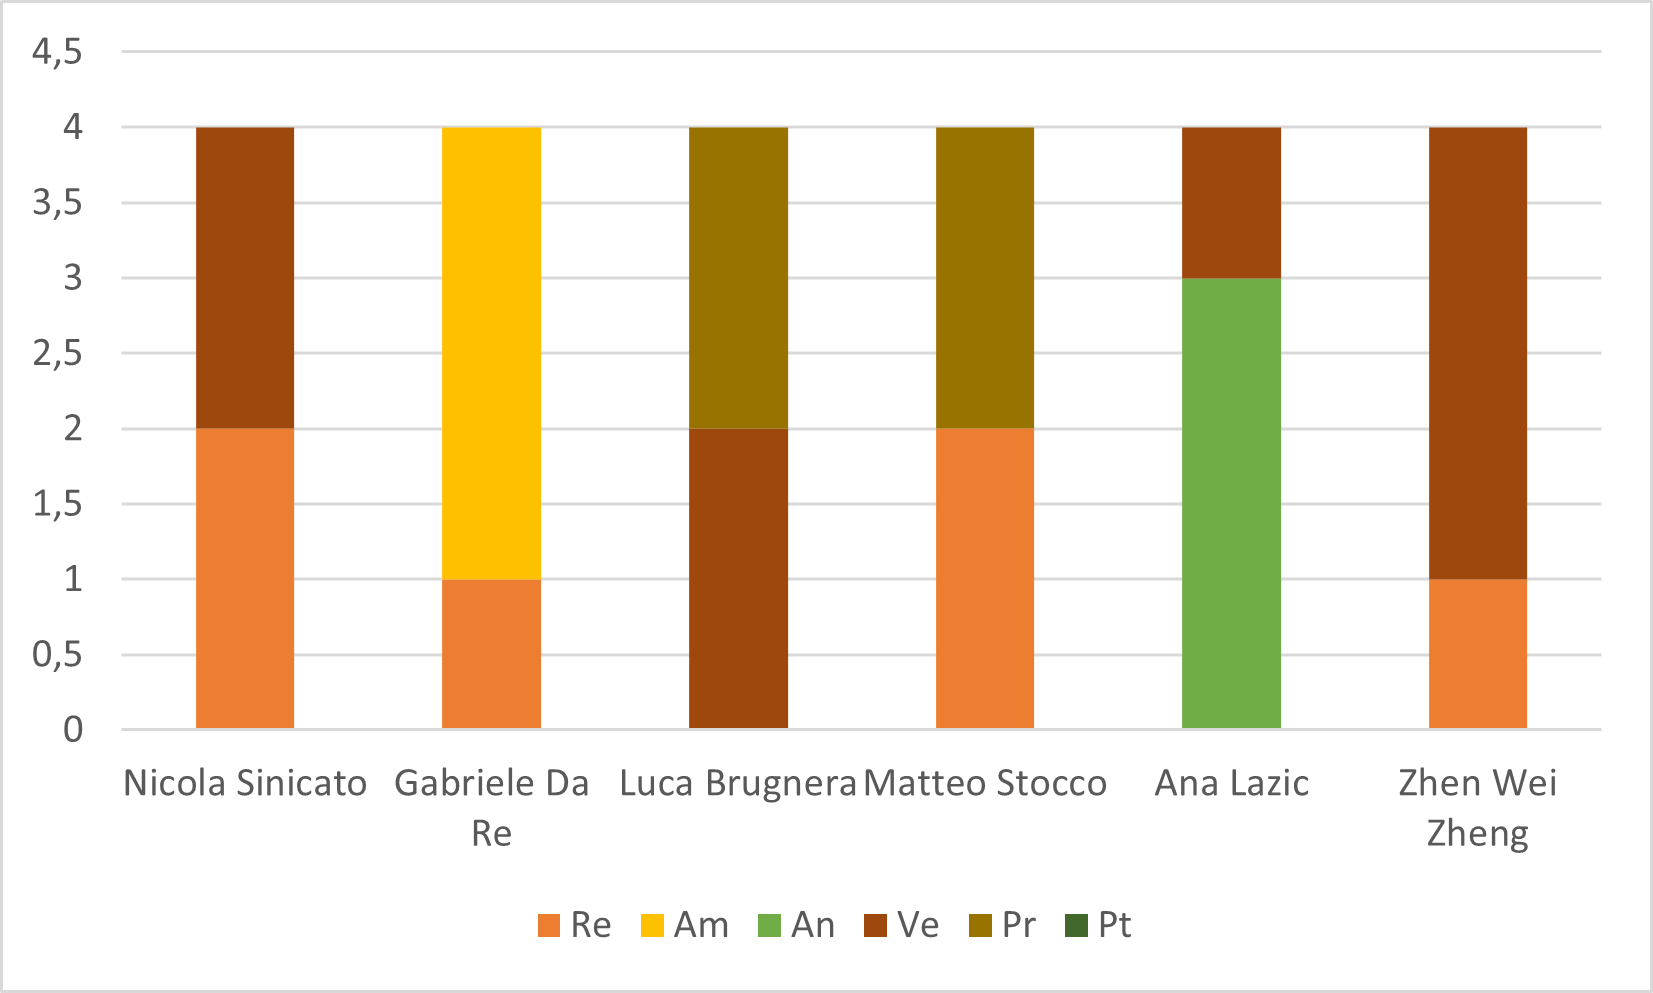
\includegraphics[scale=0.6]{img/grafi preventivo/istogrammi/validazione/periodo2.png}
    \caption{Istogramma della ripartizione delle ore del secondo periodo della fase di validazione\textsubscript{G} e collaudo}
\end{figure}
\begin{figure}[H]
    \centering
    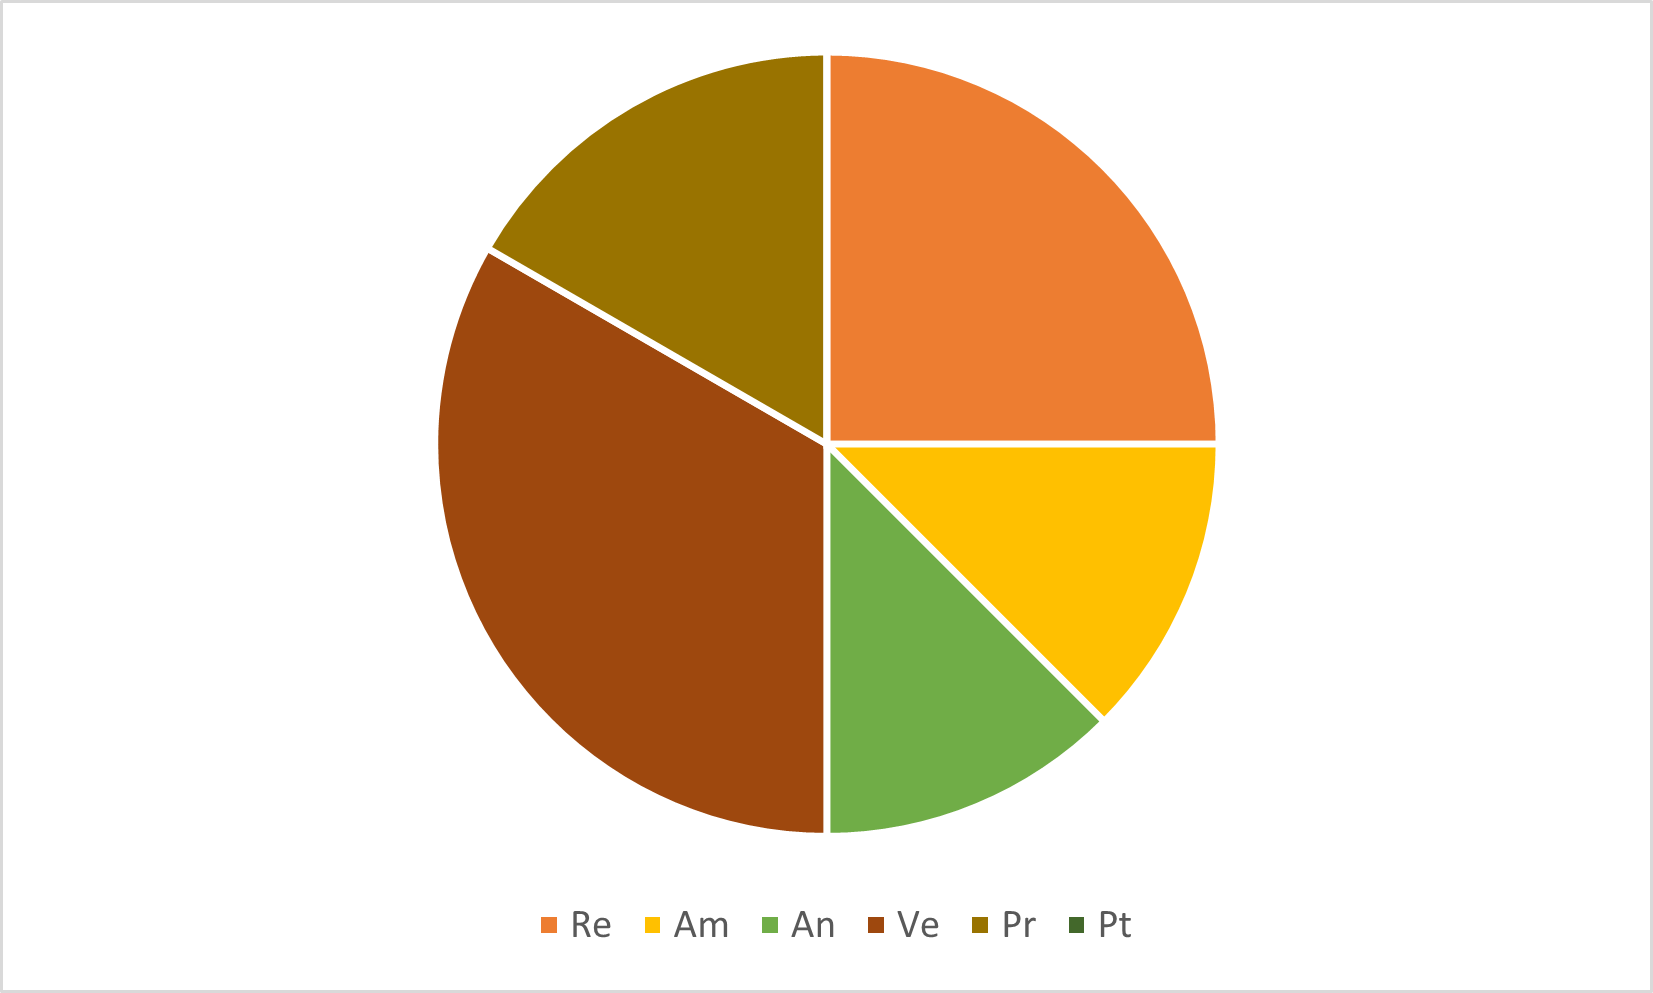
\includegraphics[scale=0.6]{img/grafi preventivo/torta/validazione/periodo2.png}
    \caption{Grafico a torta della ripartizione delle ore per ruolo nel secondo periodo della fase di validazione\textsubscript{G} e collaudo}
\end{figure}
\subsubsubsection{Preventivo dei costi}
La seguente tabella rappresenta le ore dedicate ad ogni ruolo e il corrispettivo costo in euro per il secondo periodo della fase di validazione\textsubscript{G} e collaudo:

	\setlength\extrarowheight{5pt}
	\rowcolors{2}{gray!10}{gray!40}
	\begin{tabularx}{\textwidth}{|ccc|c|}
		\hline
		\rowcolor{white}
		\textbf{Ruolo} & \textbf{Costo orario (€)} & \textbf{Ore totali} & \textbf{Costo totale (€)} \\
		\hline
		Responsabile &30&8&240 \\
		Amministratore &20&4&80 \\
		Analista &25&0&0 \\
		Verificatore &15&9&135 \\
		Programmatore &15&3&45 \\
		Progettista &25&0&0 \\
		\hline
		Totale &-&-&500 \\
		\hline
		\rowcolor{white}
		\caption{Prospetto del costo orario durante  il secondo periodo di validazione\textsubscript{G} e collaudo per ruolo}
	\end{tabularx}
    \vspace{10pt}
	
% ----------------------------------------------------------------------------------------------------------------
\newpage
\subsubsection{Riepilogo della fase di validazione\textsubscript{G} e collaudo }
% ----------------------------------------------------------------------------------------------------------------
%
\subsubsubsection{Preventivo orario}
La seguente tabella rappresenta la distribuzione oraria per ogni componente per la fase di validazione\textsubscript{G} e collaudo:

	\setlength\extrarowheight{5pt}
	\rowcolors{2}{gray!10}{gray!40}
	\begin{tabularx}{\textwidth}{|ccccccc|c|}
		\hline
		\rowcolor{white}
		\textbf{Nome} & \textbf{Re} & \textbf{Am} & \textbf{An} & \textbf{Ve} & \textbf{Pr}& \textbf{Pt} & \textbf{Ore totali} \\
		\hline
		Nicola Sinicato &4&0&0&8&3&0&15 \\
		Gabriele Da Re &3&4&0&5&3&0&15 \\
		Luca Brugnera &1&2&0&7&5&0&15 \\
		Matteo Stocco &3&2&0&6&4&0&15 \\
		Ana Lazic &4&1&0&8&2&0&15 \\
		Zhen Wei Zheng &3&2&0&6&2&0&15 \\
		\hline
		Ore totali ruolo &18&11&0&42&19&0&90 \\
		\hline
		\rowcolor{white}
		\caption{Distribuzione oraria durante la fase di validazione\textsubscript{G} e collaudo per ruolo e persona}
	\end{tabularx}
	\vspace{10pt}
	
\begin{figure}[H]
    \centering
    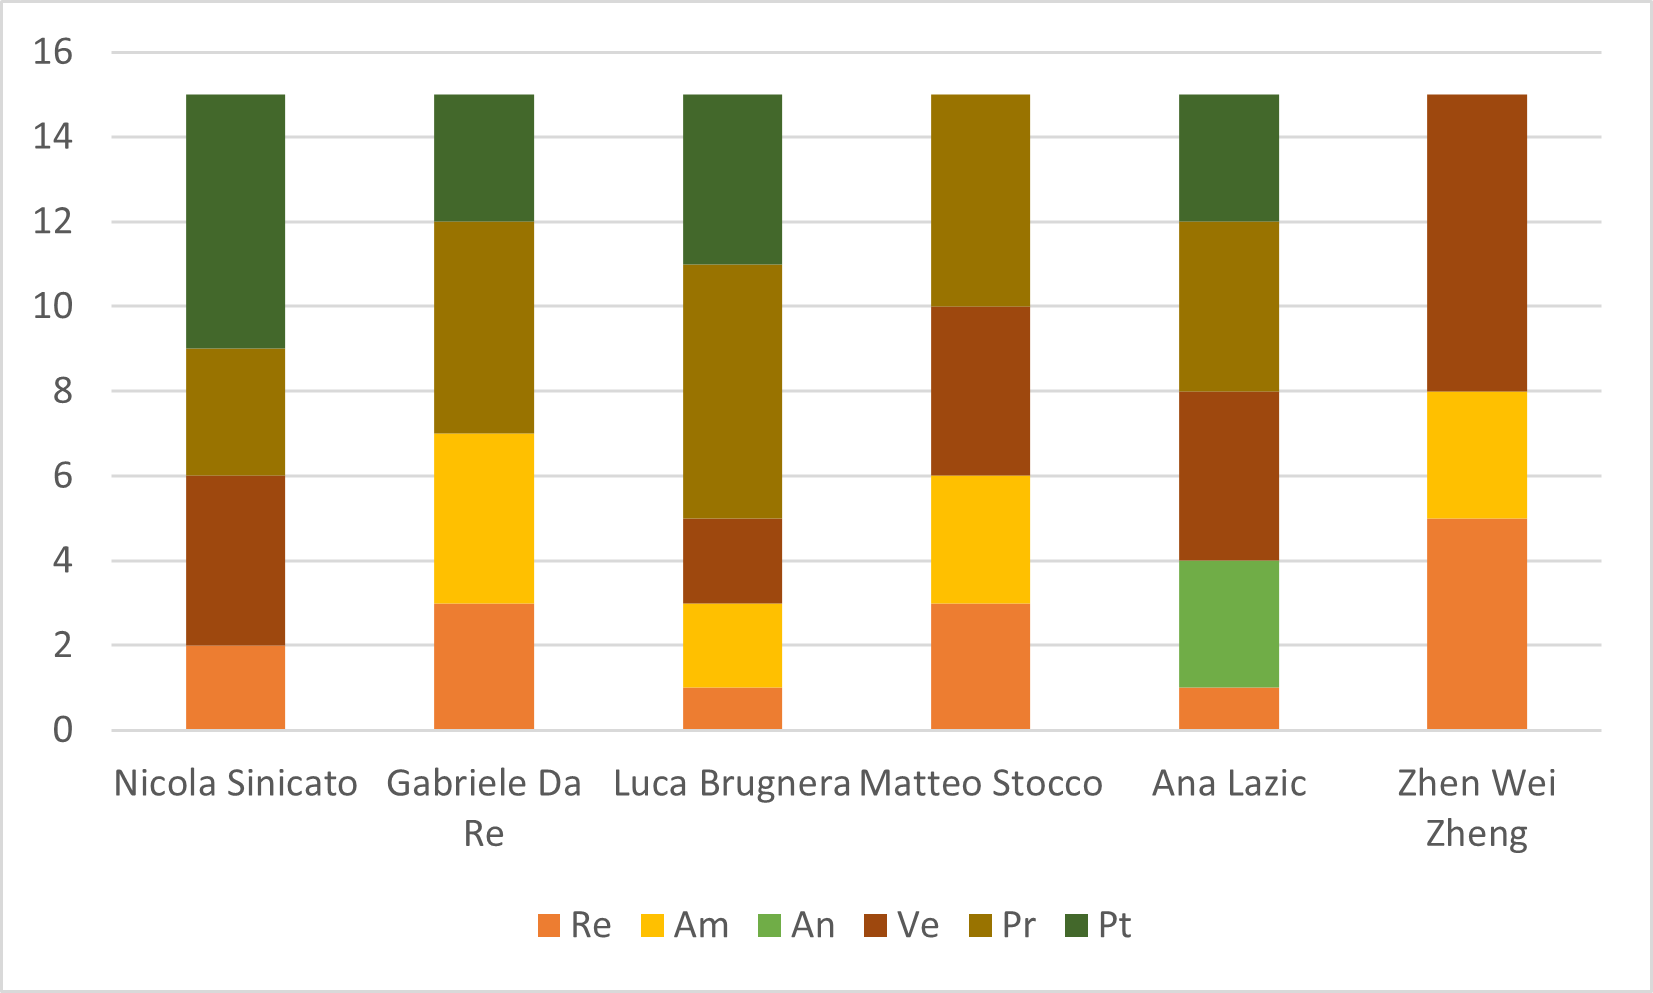
\includegraphics[scale=0.6]{img/grafi preventivo/istogrammi/validazione/complessivo.png}
    \caption{Istogramma della ripartizione delle ore della fase di validazione\textsubscript{G} e collaudo}
\end{figure}
\begin{figure}[H]
    \centering
    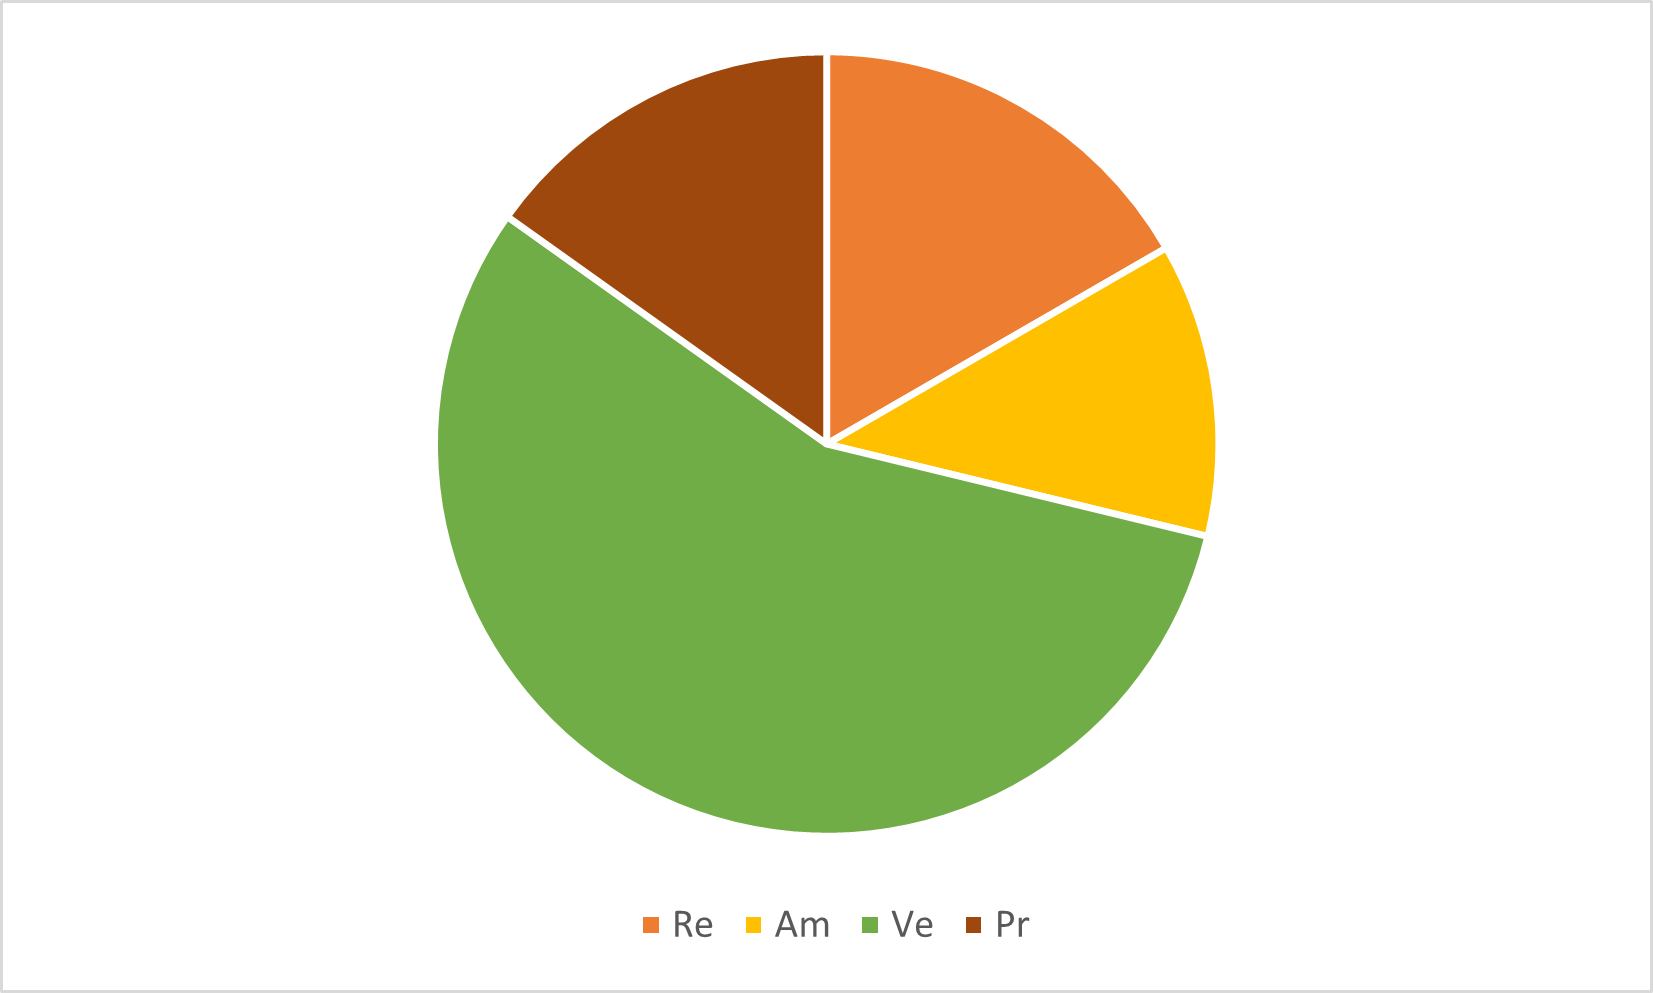
\includegraphics[scale=0.6]{img/grafi preventivo/torta/validazione/complessivo.png}
    \caption{Grafico a torta della ripartizione delle ore per ruolo nella fase di validazione\textsubscript{G} e collaudo}
\end{figure}
\subsubsubsection{Preventivo dei costi}
La seguente tabella rappresenta le ore dedicate ad ogni ruolo e il corrispettivo costo in euro per la fase di validazione\textsubscript{G} e collaudo:

	\setlength\extrarowheight{5pt}
	\rowcolors{2}{gray!10}{gray!40}
	\begin{tabularx}{\textwidth}{|ccc|c|}
		\hline
		\rowcolor{white}
		\textbf{Ruolo} & \textbf{Costo orario (€)} & \textbf{Ore totali} & \textbf{Costo totale (€)} \\
		\hline
		Responsabile &30&18&540 \\
		Amministratore &20&11&220 \\
		Analista &25&0&0 \\
		Verificatore &15&42&630 \\
		Programmatore &15&19&285 \\
		Progettista &25&0&0 \\
		\hline
		Totale &-&-&1675 \\
		\hline
		\rowcolor{white}
		\caption{Prospetto del costo orario durante la fase di validazione\textsubscript{G} e collaudo per ruolo}
	\end{tabularx}
    \vspace{10pt}
	
%

% ----------------------------------------------------------------------------------------------------------------
\newpage
\subsection{Riepilogo complessivo}
% ----------------------------------------------------------------------------------------------------------------
%
\subsubsection{Preventivo orario}
La seguente tabella rappresenta la distribuzione oraria totale per ogni componente:

	\setlength\extrarowheight{5pt}
	\rowcolors{2}{gray!10}{gray!40}
	\begin{tabularx}{\textwidth}{|ccccccc|c|}
		\hline
		\rowcolor{white}
		\textbf{Nome} & \textbf{Re} & \textbf{Am} & \textbf{An} & \textbf{Ve} & \textbf{Pr}& \textbf{Pt} & \textbf{Ore totali} \\
		\hline
		Nicola Sinicato &12&9&14&20&24&11&90 \\
		Gabriele Da Re &9&21&12&14&18&16&90 \\
		Luca Brugnera &4&19&15&18&21&13&90 \\
		Matteo Stocco &9&12&14&23&22&10&90 \\
		Ana Lazic &10&10&16&20&19&15&90 \\
		Zhen Wei Zheng &9&12&15&28&13&13&90 \\
		\hline
		Ore totali ruolo &53&83&86&123&117&78&540 \\
		\hline
		\rowcolor{white}
		\caption{Ripartizione globale delle ore per ruolo e persona}
	\end{tabularx}
	\vspace{10pt}
	
\begin{figure}[H]
    \centering
    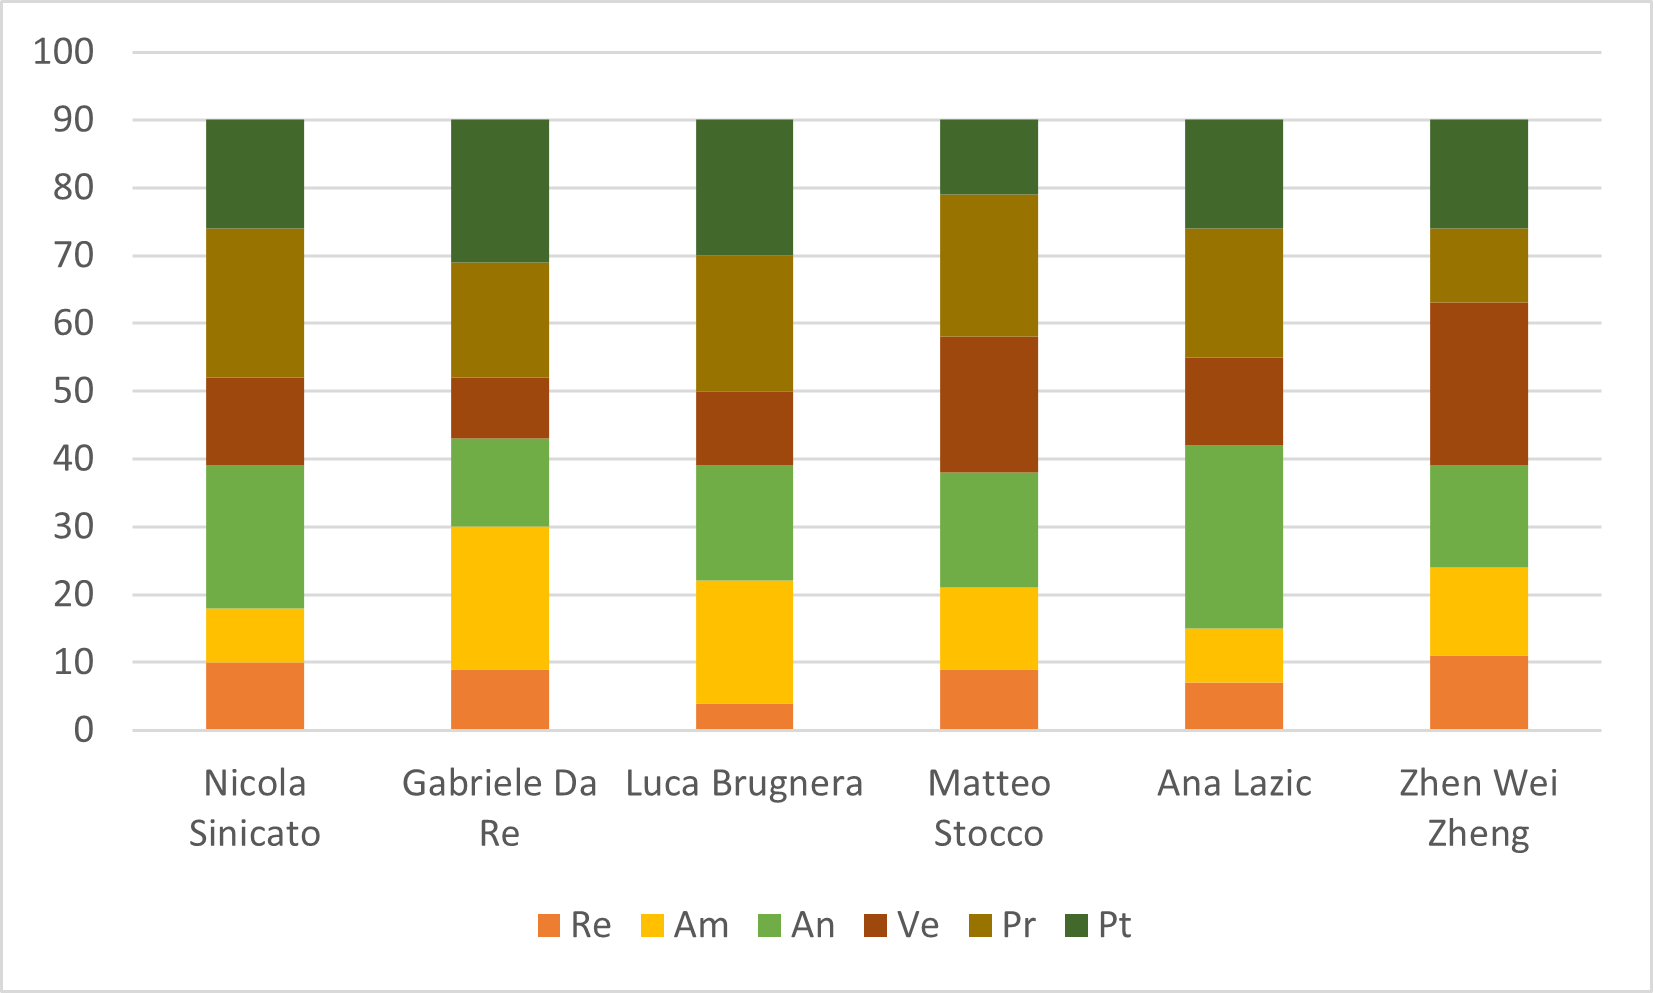
\includegraphics[scale=0.6]{img/grafi preventivo/istogrammi/totale/totale.png}
    \caption{Istogramma della distribuzione oraria}
\end{figure}
\begin{figure}[H]
    \centering
    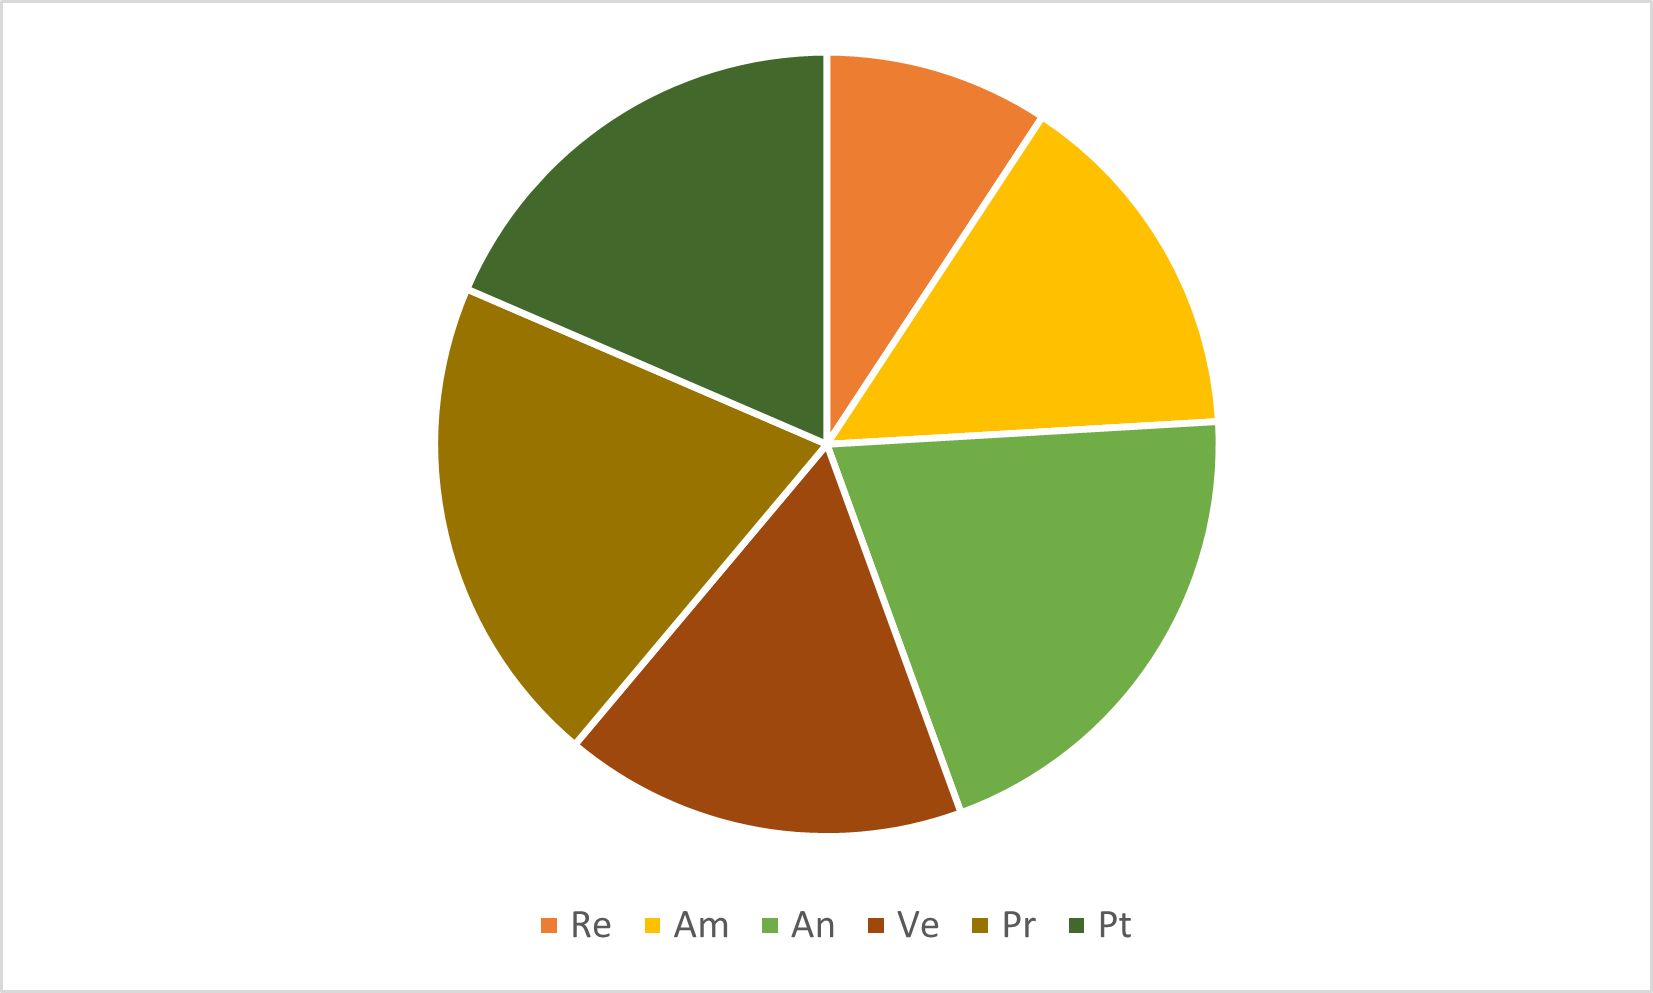
\includegraphics[scale=0.6]{img/grafi preventivo/torta/totale/totale.png}
    \caption{Grafico a torta della ripartizione delle ore per ruolo}
\end{figure}
\subsubsection{Preventivo dei costi}
La seguente tabella rappresenta le ore totali dedicate ad ogni ruolo e il corrispettivo costo in euro:

	\setlength\extrarowheight{5pt}
	\rowcolors{2}{gray!10}{gray!40}
	\begin{tabularx}{\textwidth}{|ccc|c|}
		\hline
		\rowcolor{white}
		\textbf{Ruolo} & \textbf{Costo orario (€)} & \textbf{Ore totali} & \textbf{Costo totale (€)} \\
		\hline
		Responsabile &30&53&1590 \\
		Amministratore &20&83&1660 \\
		Analista &25&86&2150 \\
		Verificatore &15&123&1845 \\
		Programmatore &15&117&1755 \\
		Progettista &25&78&1950 \\
		\hline
		Totale &-&-&10950 \\
		\hline
		\rowcolor{white}
		\caption{Prospetto del costo orario per ruolo totale}
	\end{tabularx}
    \vspace{10pt}
	
% ----------------------------------------------------------------------------------------------------------------
